%\documentclass[ebook,12pt,openany]{memoir} %add onesided in square brackets for a real ebook(non printed)

\documentclass[ebook,12pt,openany,onesided]{memoir} %add onesided in square brackets for a real ebook(non printed)

\usepackage[utf8x]{inputenc}
\usepackage[english]{babel}
\usepackage{url}
\usepackage{graphicx}
\usepackage{imakeidx} % for how to use the index see https://www.sharelatex.com/learn/Indices

\makeindex




\title{Trash Magic \\ Book I: Manifesto, Activity Book and Coloring Book}
\author{Lafe Spietz}

\begin{document}
\frontmatter
\begin{figure}[htbp]
\centering
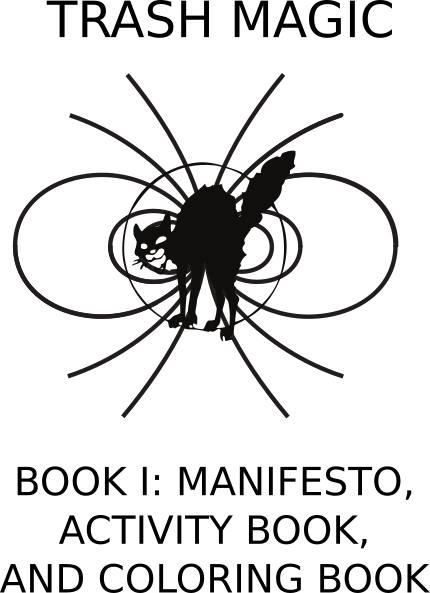
\includegraphics{images/frontcover2.png}
\end{figure}

\clearpage

\clearpage



\newpage
\thispagestyle{empty}
\mbox{}

\begin{figure}[htbp]
\centering
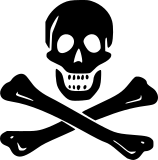
\includegraphics{images/jollyroger.png}
\caption{NO PROPERTY}
\end{figure}

\subsection{INTELLECTUAL PROPERTY
NOTICE}\label{intellectual-property-notice}

ALL WORK CREATED HERE IS THE PRODUCT OF A PERSON OR PEOPLE WHO DO NOT
RECOGNIZE THE VALIDITY OF ANY INTELLECTUAL PROPERTY OR INDEED ANY OTHER
PROPERTY LAW. NO RESTRICTIONS BASED ON SUCH LAW ARE HERE DECLARED OR
RECOGNIZED. ALL USE BY ANYONE WITHOUT ANY RESTRICTION INCLUDING FOR
COMMERCIAL PURPOSES IS ALLOWED, SINCE NO LAW IS REFERENCED AT ALL IN
THIS DOCUMENT. THIS IS A SELF-ANNULLING DOCUMENT, IN THAT IT IS INTENDED
TO CARRY NO LEGAL WEIGHT AND TO SERVE AS A SUBSTITUTE FOR A LEGAL
DECLARATION AND A NEGATION OF ANY POTENTIAL LEGAL CLAIMS. NO LIABILITY
BASED ON CREATIONS HEREIN ARE RECOGNIZED BY THE AUTHOR. NO LAW OF ANY
KIND IS RECOGNIZED BY THE AUTHOR.

NO PATENTS

NO COPYRIGHTS

NO LAWS

NO MONEY

NO MINING


\maketitle

\tableofcontents

\listoffigures 

\mainmatter
\chapter{Capitalism}
What is best in life?

To care for one another, and to have adventures.

Technology can help us do both of these things, building societies where
all physical needs are taken care of as well as which preserve the
adventure that makes life worth living. However, as technology has
advanced it has increasingly served its own needs. Because it has had
such a powerful overall positive effect on the human condition(in some
material ways), we have allowed the rules of technical progress to
dictate the rules of the rest of our society. In this chapter I discuss
how I view capitalism as an underlying force which drives this process,
creating great suffering for humanity and the rest of the living world.

\subsection{What is Capitalism?}\label{what-is-capitalism}

What is capitalism? This is something that critics of it avoid a lot of
the time to their detriment. If you look up various definitions, it
generally goes something like this: ``Capitalism is the economic system
in which the means of production are privately owned.'' I hate this
definition, and I think it's held back our collective effort to fight it
for the last 150 years.

What this definition implies is that the opposite of capitalism is
someone other than ``the private owners'' or ``the capitalists'' owning
the ``means of production'', and ``economics'' being based on something
other than private capital. I put all these things in scare quotes
because I see them all as subtle weapons to inject hidden ideology into
peoples minds by the very wording of the definition. First of all, the
anarchist rejection of capitalism rejects ownership of minerals, land,
and machines. So any definition that talks about ``who owns what''
should already be rejected by the anarchist, and we have already ceded a
major point by allowing this definition to stand at all unexamined.
Capitalism is a system in which some people, called ``owners'', claim to
have power over certain things which they claim the right to carry out
by force if needed. Capitalism is a system in which a military state
exists which both feeds of the system of privately owned extraction and
enforces the power structure that governs it.

The ``means of production'' is also a problematic phrase. While it is a
bit ambiguous, I see this phrase as at least potentially implying that
this the ``means'' is some sort of fixed infrastructure. The implication
is that ``the means of production'' is a thing that exists outside of
economic systems, which can be controlled by any of various types of
government or state. This is false. The very structure of ``production''
in today's society is what I would call capitalism. The Soviet system,
the various fascist systems, ``democracies'', dictatorships, monarchies,
I would say every single one of them is capitalist. They all have this
basic structure of military power creating a monopoly of force that
protects a vast system to extract mineral wealth and destroy it as fast
as possible by constant threat of violence. To me calls to ``seize the
means of production'' sound like calls against a king to go seize the
palace and tell the king what to do but to keep the palace and king in
place. It's the same system, with slight changes. So to let the
capitalists define these ideas gives them a victory before a debate even
begins: it allows that the existing ``means of production'' should
continue to exist without discussion. A true challenge to capitalism is
one in which the very concept of production is reinvented. It means
building industrial technology from the ground up around different
values.

Another problem is with the notion of ``economic system''. I would argue
that economics is again a part of the intellectual descendent of the
basic idea of the One God of monotheists. There is a Universal
Heierarchy that exists, which allows numbers to be used to assign value
to things. Human value becomes a number, always either less than or
greater than or equal to any other numerical human value. Part of
rejecting the basic ideas of capitalism is to reject this hierarchy cast
down from God. But to even use the phrase ``economic system'' again lets
capitalism be defined in a universe in which nothing other than
capitalism exists.

Indeed in some of the definitions I've found online they even add
phrases like ``as opposed to State ownership of the means of
production''. In other words the supposed definition of capitalism used
by most people is not a definition of capitalism at all, but a clever
propaganda piece that creates a world in which the alternative to
capitalism is another type of capitalism which is re-cast as the
Socialist Enemy. Since I consider all the Soviet style ``communist''
countries to be capitalist in their philosophical worldview, I find it
not surprising that they hold the same warped view of this false
dichotomy. The communists can point to ``capitalism'' as their enemy,
where ``the ruling class'' ``own'' the ``means of production'', rather
than ``the dictatorship of the proletariat''. When this becomes a
nightmare like it always does and destroys the environment even worse
than ``capitalism'', people on the right say ``I told you so'' and
people on the left say ``it will be different next time! it's all
Stalin's fault!''.

So if we really want to move beyond capitalism, criticisms of it need to
start trying to really see it for what it is, and see just how far the
viral ideas about God that underly it have wormed their ways into the
very language we use to describe it.

I will give capitalism the following definition:

\textbf{Capitalism is a system of belief in which numbers are used to
denote all value.}

That, I believe, is the heart of the matter. And it points to why
experiments like the USSR have ended up having problems so similar to
those in the western capitalist world. In a word, money. Money is not
just metal or paper or faith in a government, it is the idea that a
number, specifically an integer number(money can usually be subdivided
but only up to a point) can be used to denote all human values. This is
why I believe the concept is so slippery, and so hard to break out of.
You can replace dollars with time dollars, bit coin, gold, silver, bags
of salt or gold-backed e-dinar and it's really all the same thing:
numbers. Integer numbers. As long as there is an exchange rate between a
system of value and an existing currency you have not really broken free
of the current system.

\begin{figure}[htbp]
\centering
\includegraphics{images/bigone.png}
\caption{Worshipping the Number One}
\end{figure}

And what is money? The purity of numbers has proven to be incredibly
powerful. Users of the number based values have literally moved
mountains with the power they have been able to deploy using money. In
particular money based values have been excellent at several things,
some of which are good but most of which are bad. I will now explore the
nature of money more specifically.

\subsection{The Nature of Capitalist
Money}\label{the-nature-of-capitalist-money}

\begin{figure}[htbp]
\centering
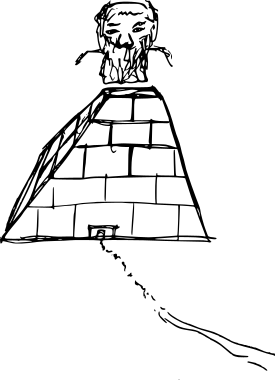
\includegraphics{images/capitalpyramid.png}
\caption{Suffering and Minerals}
\end{figure}

Our currency is based on two things:

\begin{enumerate}
\def\labelenumi{\arabic{enumi}.}
\item
  suffering
\item
  and minerals
\end{enumerate}

Turning minerals and human misery into numbers is capitalism in a
nutshell, and is the basis of our monetary system.

\begin{figure}[htbp]
\centering
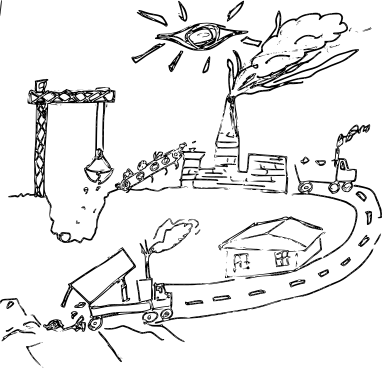
\includegraphics{images/digitup.png}
\caption{Dig it up, set it on fire, and bury it}
\end{figure}

Capitalism is an industrial system in which all value is based on human
misery and minerals. By creating misery, some people use threats of
violence to control land. They use more minerals, fire, and misery to
create minerals ordered with a precision based on their belief in
violence and control through military order. The threat of inflicting
misery using military technology(not only is our technology military,
our concept of military is based on our technology as well, and both are
based on the One God beliefs) is how some people known as capitalists
claim ``ownership''. Ownership is a complex network of violent threats
which allow threats of future misery and benefits paid from past misery
to be added up numerically, building a ladder of power down which the
physical benefits of mineral wealth slowly trickle, with the most
landing at the top.

Any proposal to reform capitalism that maintains concept of numerical
adding up of suffering and minerals is just capitalism with a new mask
on. True reform means finding a set of moral values that informs
technological figures of merit which are based on human joy, adventure,
hilariousness, beauty, or other things that actually have positive value
for everyone, and then re-builds our whole concept of what it means to
have a technology up from scratch.

To repeat: to attempt to reform capitalism while continuing to use any
of our current technology at all is a lost cause. The ideas of
capitalism are built into the position of every atom in a modern
technical artifact. If you want a world without capitalism you must re
order every atom, completely re design how atoms go together from the
bottom up. And in building this it makes sense to acknowledge that
300-400 years of industrial capitalism gave us the gift of minerals,
which we can now live on forever.

Every atom. Every atom changes in how it relates to the whole. Same
physics, same atoms, but new ordering principles, breaking out of the
military design concepts. No more are the ideal shapes always planes,
circles, and perfect grid arrays of objects. No more are tech artifacts
locked into a centrally controlling clock that tells them when to work
and what to do. No more is there a wall between engineer and customer,
where some things are known and some are secret: all information on
construction is physically encoded in the artifact, and updated as more
edits are made, even if the user does not document(data stream into the
dataverse).

\subsection{Capitalism as Religion}\label{capitalism-as-religion}

Capitalism is the hidden religion. It does not admit to being a religion
and its believers(at this point almost all humans) do not realize they
are in this religion but they are. Even members of various other
religions decry people leaving their flocks for the ``secular'' world
but won't directly name this as a competing religion. But a religion it
is, complete with odd beliefs of all kinds.

In my observation, the beliefs of capitalism include:

\begin{enumerate}
\def\labelenumi{\arabic{enumi}.}
\tightlist
\item
  Private property is sacred
\item
  All value can be added up using numbers
\item
  All value must be extracted from the Earth or from human misery
\item
  Human society is described by something called an ``economy'', which
  is a system for laundering mine products and human misery into
  numerical media of exchange
\item
  Hard work is an intrinsic good
\item
  Our world can all be described by a giant hierarchy, people, animals,
  objects, gods, ideas, all are always ranked and this ranking is
  ordained by the highest authority, whatever that is.
\end{enumerate}

I believe that number worship is an underlying hidden religion that is
integrated into all other modern mainstream capitalist religions. What
is monotheism? It is the belief that there is only one true god. But
this implies that you can count gods. That is the underlying assumption.
It separates parts of the universe that are god from non-god in a rigid
way, breaking up gods or potential gods into discrete numbers that one
can count, rank, and ultimately then put one on top of all others. From
this we get hierarchy of all kinds down through the ages and all the
horrors of capitalism. But if you are a monotheist note that your One
True God is almost certainly also a universal part of your world. So
what makes you believe you can count gods? This other, hidden, religion
that is required to phrase the questions and answers about your god
using numbers. So do not take my attacks on the structure of industrial
monotheism as an attack on your One God--I do not deny your god, merely
your ability to count gods.

That being said, I do think this counting has led to other problems in
industrial monotheism which must be combated, namely patriarchy.
Monotheistic religions have a strong tendency to extend the counting
hierarchy from their bearded man-god down to all Things, building an
instant patriarchy into their world view. Don't do that!

Number worship, the belief in numbers as a superior picture of reality
than other models. BBC documentary on history of numbers is actually
blatant capitalist religious propaganda nonsense. Vietnam war, big data,
the very word ``rational'', always the assumption that number-based
ideas are superior than ideas not based on numbers.

\subsection{Professionalism: A Capitalist
Cancer}\label{professionalism-a-capitalist-cancer}

I am against professionalism in all forms. Professionalism divides us.
We have split up philosophy, physics, chemistry, biology, design,
manufacturing, theology, art, and technology, and very much to the
detriment of them all.

I'm against engineering and design as professions. While specialization
can be useful, I believe our society has created a soul-less
techno-priest class which is evil enough in its very nature that
technology needs to be re-built from the ground up outside that system.
If your technology needs the techno priests to function, it means your
technology is bad and needs to be replaced. If it needs extraction of
raw materials from the earth or any control over large tracts of land in
a centralized way to function it is bad technology and needs to be
replaced. If it requires secrecy or proprietary control of information
and use it is bad technology. If it can't function without capitalism it
is bad technology and needs to be replaced.

Specialization is fine up to about 100 people then it is a luxury for
special projects. If you need someone who makes up less than 1\% of the
population to do something your technology needs a reset and it is bad.
Our goal is total freedom for 100 people.

We need to start over from scratch and build a technology without the
existing techno priests which can be built and maintained by anyone with
the desire to do so, using waste streams of the old system. This has to
happen in thousands of parallel tracks in many different fields of
applied science and technology. I will focus on the parts relevant to my
area of expertise: applied physics.

\subsection{Capitalism Stifles
Innovation}\label{capitalism-stifles-innovation}

Part of what has led me to write this work is my frustration as a
professional scientist with how capitalism has, in my view, held back
scientific, technical and cultural innovation by decades if not
centuries.

There are several aspects of capitalist ideology which have had
devastating effects on science. The first is the obsession with novelty.
This is probably the largest problem, which I would say has gotten
progressively worse as science got more advanced over the last 100 years
or so. The problem is that in order to be seen as a success in science
you need to prove that what you did is really new, and that newness
takes priority in value over almost everything else. What this does is
create a very broken ladder of importance of things to study. If you
have the choice between two experiments which both show the same
science, and one involves just seawater, dirt, and a mobile phone, and
the other involves a 1 million dollar machine, a trendy new molecule,
and some advanced math using a new computer algorithm, the latter is
considered vastly superior. And this is based on the ideology of private
property, even when legal intellectual property is not involved. Even in
the public domain, when a researcher publishes a sufficiently new thing,
that thing is attached to their name, and can be turned into real
tangible monetary value.

All the elements I describe in the example above should be called out
for causing problems with science progress. First of all, the use of
expensive machines. This not only makes sure there is a barrier between
the work of the lab scientists and the general public, it usually
increases the distance between the researchers themselves and the
subject matter. I believe that the purpose of all science is to create
the closest possible link between the human mind and the world we live
in. The more expensive your machine, the larger the barrier between mind
and world. Expensive machines are great for building capitalist
jobs(I've had these jobs!) But this is at cross purposes with what
should be the goal of simplification. To eliminate a machine is to
eliminate a high paying technical job, which hurts us as workers in
science. Thus the incentive is opposite of what we want to do, which is
always cut down the the size and number of machines needed to interact
with our world.

Another element of the problems I've listed here is the ``trendy
material'' problem. That is, science is strongly biased in favor of
newly ``discovered'' materials over those we all know and have access
to. This is created by capitalist ideology because we all need to try to
own the property, both legally and intellectually, of ``new'' things in
order to get the fame required to advance in our careers. If you prove
that ``your'' substance has a different chemical structure than any that
someone else has studied, and publish something not very impressive, you
can get famous, and name the molecule. But if you do something
impressive, but not really new, on something common like tap water or
ground up moss or a soda can, you have to call it ``educational
demonstrations'' and will not be taken seriously in high level research
circles. But again, this is creating an incentive to do the opposite of
what is good for science. Someone who interacts with tap water or
pavement has a connection to much larger fraction of the world than
someone who interacts with an obscure form of soot made in a special
chamber that only exists in their lab. If our goal is to connect our
minds to the world as well as possible, it's always better to follow the
most common elements of that world, then things we find around us.
Capitalism pushes the researcher away from those things both because of
the need for novelty and also because the more obscure a molecule is the
more likely it is that a capitalist can make a profit on it. A product
based on a simple recipe with tap water and gravel is worth infinitely
less money than one based on a complex and expensive process.

The ephemeral concepts of ``ownership of ideas'' above pale in evil
compared to legal intellectual property. This could be a whole polemic
work of book length on its own but suffice it to say that the corrosive
effect excessive patent and copyright are now so severe that anyone
who's worked at all in science in the last 10 years is already pretty
upset about this issue. Even those who claim to support the system agree
that it's now so far beyond even the twisted intent that originally
existed that they are against it in its current form. However, for the
record, my position in this work is that it is pure evil to claim the
concept of ownership over science or technology. The scale of the evil
is partly escalating as the technology becomes more personal. As our
technology becomes more a part of not just our lives but our selves, we
find corporations claiming to legally own parts of our lives and even
our bodies with their patenting of genes both in humans and in our
various bacterial neighbors we carry on our bodies. Eventually, the
property ideologues will, if left unchecked, build a world where humans
are all owned by a consortium of corporations, where we are all
literally the property of corporations and machines. Science fiction
warns of the possibility that a ``rise of the machines'' will cause us
all to become slaves to artificially intelligent machines, but I would
argue that AI is not needed for us to become slaves to machines:
humanity is in the process of enslaving ourselves to non-intelligent
machines.

I touched on the problem of professionalism already but I need to
elaborate on this in the context of science specifically. We have always
claimed in philosophy and science that unification is a goal.
Unification of electricity and magnetism into one theory and then the
weak force in with that are all seen as great triumphs of physics.
Bringing all the atomic elements together into a single unified periodic
table is rightly seen as a great triumph of chemistry, etc. But in
modern applied science we find huge incentives in the opposite direction
of unification. Because we are all forced to carry out science in the
professional system, and there are never enough professional positions
to go around, those with the good professional jobs must all jealously
guard our positions. This means a biologist who can do good physics or a
physicist who can do good biology are both potential threats to each
others' jobs. Whereas the biologist who creates an even more obscure
form of biophysics that gets its own whole new department is the most
powerful of all: the unique specialist who owns their field entirely.
The highest salaries and most honored and secure positions will go to
those who do the opposite of unification. And sure enough, the last few
decades have seen a proliferation of tiny sub-fields with their own
jargon no one else can read in all fields of science. This has coincided
with the rise of extreme market ideology since the 1970s which drives
universities to behave more like businesses and research departments to
behave more like marketing departments. The corrosive force of
capitalism has inflicted a sort of Babel curse on all science, making it
impossible to talk to each other anymore.

This concept of unification applies in particular to building the tools
we use for science. The most useful tools are the most universal: razor
blades, tweezers, optical microscopes, or pliers. And yet no
professional scientist can make a living selling any of those, so we're
not incentivized to make more tools like those. We can make them for our
own use in our labs, but capitalism directs those types of tools to be
made by the cheapest possible labor, so building them is avoided by the
professional classes. Conversely, the tool which only does one thing
extremely well can be a perfect monopoly on that thing, creating a large
markup and building a comfortable place for the professional. Again this
is a case of capitalist ideology constantly pushing us all to build the
opposite tool from what would benefit our fellow scientists or the rest
of humanity.

These claims are just claims when stated in a a manifesto like this. I
state them without extensive proof because the proof that abandoning
capitalism can push science and technology forward much faster has to be
by example. We must actually go out and do this, build science and
technology up from scratch on non capitalist principles, without
professionalism and without property. Ultimately this ends up looking
more like an artistic movement(for which a manifesto would be a normal
part of the creation process) than a part of science. Trash Magic will
take many forms in the future, but its initial form will indeed be that
of an artistic movement, because that's the simplest way to build things
while casting off the old figures of merit used by engineers and the
rest of the technocratic priesthood.

\subsection{Death to Capitalist Math!}\label{death-to-capitalist-math}

Math is not objective reality. This is obvious to most people who don't
do math, as well as to most working mathematicians, but it's an
amazingly popular belief among technocrats. Math, like any other model
built in the human mind, is a sort of reflection of the world. A very
powerful one, yes, but still just a part of our minds, and like any
other model, there are choices we made to get where we are with math
which could have been made differently.

The example I'll give here is a paradox that I find particularly
interesting in terms of what it tells us about hidden ideologies.
Mathematicians call it the Banach Tarski paradox, and it generally
arises in parts of the math curriculum concerned with point set theory.
Never mind exactly what that is, it's something usually taught in the
late undergrad or early grad level in pure math(as opposed to applied
math which is not concerned with these issues).

\begin{figure}[htbp]
\centering
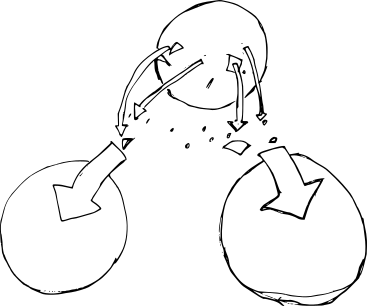
\includegraphics{images/banachtarski1.png}
\caption{Construction of Banach Tarski paradox}
\end{figure}

What this so-called paradox does is create a way to construct two
spheres of points from the points in one. That is, all the points in the
first sphere are re-arranged in such a way that those same points make
two spheres of the same volume as the first.

\begin{figure}[htbp]
\centering
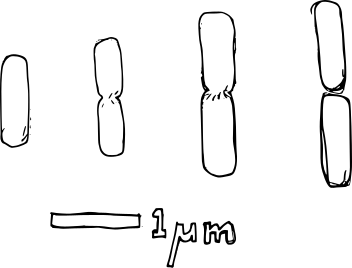
\includegraphics{images/ecoli.png}
\caption{Biological Cells Ignoring Math and Capitalism}
\end{figure}

\subsection{Why Now?}\label{why-now}

Now is the time for \emph{drastic} change unique in our history.

Why now in particular?

Both the positive and negative sides: danger to humanity is imminent,
but also opportunity is greater than ever before because of the vast
mineral wealth that is everywhere and a critical mass of processing and
communication technology. Marx was about 100 years early, and didn't
have access to the information or materials we do today. Globalization
and Capitalism really have literally sewn the seeds of their own
destruction, by creating seeds for millions of new societies by
spreading mineral wealth everywhere around the globe.

The very destruction of capitalism focuses us on the better future in
several ways. For one thing, the sections of society most exploited or
crushed by capitalism are often also those closest to the massive waste
and destruction streams of the present system. Often the poor and
dispossessed live near dangerous waste which also contains what could be
priceless mineral wealth if we had the technology to bring it back.
Wherever you find the most oppressed people you will also usually find
the most ruined land with the most material waste. Just like the people
our economy casts aside, these materials often exist outside the
ownership system, they are claimed by no one and valued negative or not
at all by our economic system. But this creates a potential opportunity
to build very rich new forms of industry that exist without ownership or
money: built by people who no one pays, made from materials considered
``toxic waste'' by the ownership society, and given freely to a
community who also owns nothing undermines the entire structure of the
existing system.

This connection between the people and the materials cast aside is what
Trash Magic is really about. People who's time capitalism does not value
can use the materials it does not value to truly work magic: to build
great works of art that we can live off of using the powers of our
minds.

\subsection{Purpose of this Book}\label{purpose-of-this-book}

This book is a manifesto. That is, ``\ldots{}a public declaration of the
purpose, principles, or plan of action of a group or individual.'', as
it's described on manifestos.net.

Note that novelty is not my goal. I believe that the obsession with
novelty in applied science is a toxin of capitalism and that by ignoring
where ideas come from and using them as needed, with no expectation of
novelty that much faster and better progress can be made. This work
comes from the heart and mind of one person but none of that comes from
just me: I assume everything I say here has been said elsewhere and that
I've been exposed already to most of what I present here, in various
forms, in books I've read or from people I've talked to.

\subsection{Paths Out of Capitalism}\label{paths-out-of-capitalism}

I'm against the machine. That's what this is all about. I hate
industrialized society, and I resent that the good products of it are
used to hold us all hostage to the totality of The Machine. The military
machine, the capitalist machine, the consumerist machine, the extraction
of raw materials machine, the political machine, all of it. We're told
that if we it's all or nothing. Don't like nuclear bombs? No vaccines
for you. Sick of the Internet giants controlling your life? Well, I hope
you like writing letters by hand, asshole, you must be a Luddite. That's
the message over and over from the mainstream of society.

I challenge all that. I say that the course of the last 300 years of
industrial development has not been just fixed by some immutable laws of
nature but has in fact been the product of decisions made which could
very well have been made differently while still learning how the world
works and how to make useful technology to better navigate that world.

\newpage
\begin{figure}[htbp]
\centering
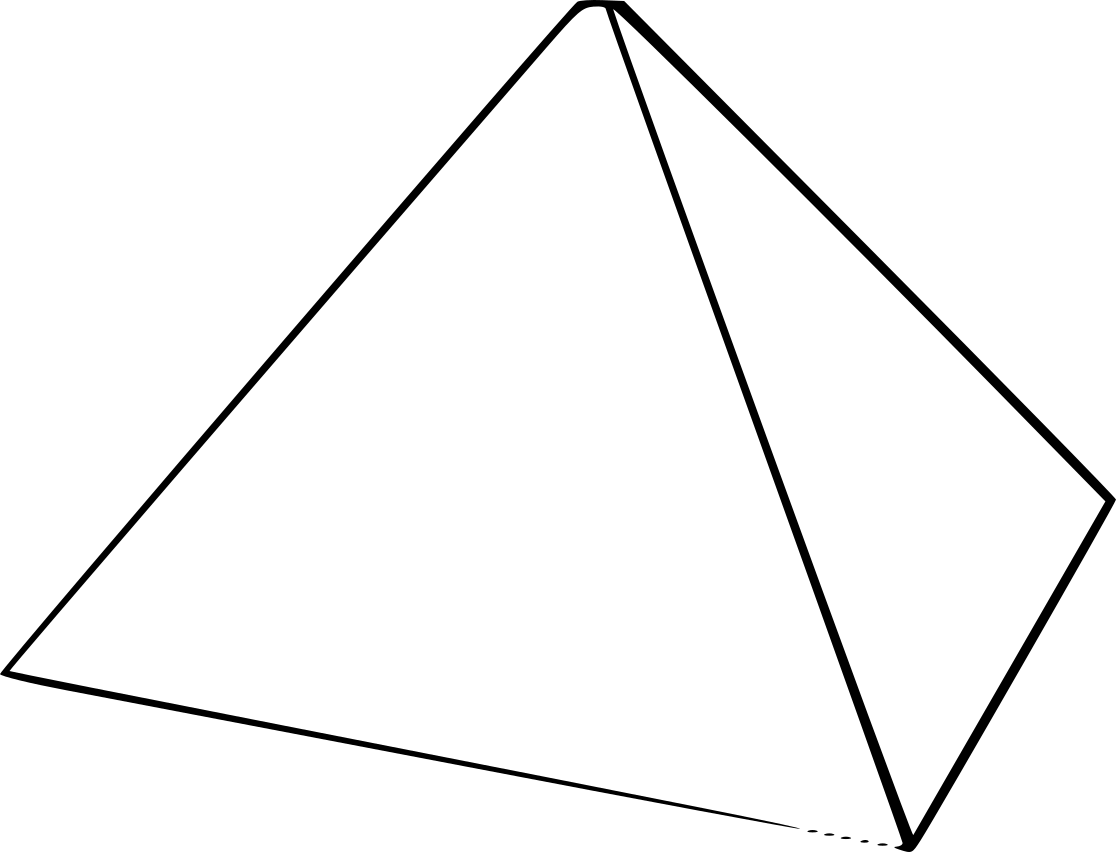
\includegraphics{images/contemplations/contemplation1C.png}
\caption{First Contemplation}
\end{figure}

\subsection{First Contemplation: Pyramid of
Capitalism}\label{first-contemplation-pyramid-of-capitalism}

In the first contemplation we contemplate the evils of capitalism
through the lens of the pyramid, a universal symbol of that ideology.

Go out in your city and look at the ways capitalism worships itself.
Banks, giant office buildings of corporations, luxury hotels, old parks,
and court houses all show huge mounds of very precisely cut stone as
part of the system of worship of stone and order that we see in the
capitalist world. Go stare at them! Marvel at both how beautiful and
majestic they can be and how much evil the also symbolize with their
cold, impersonal stone. Note that these stone monuments are almost
always accompanied by surveillance cameras, a jarring reminder of what
they mean in our modern world.

The Contemplation can also be carried out at home by placing the pyramid
in front of a small capitalist artifact, playing the proper music, and
vigorously flopping around on the floor in ALL DIRECTIONS while
maintaining eye contact with the pyramid and evil artifact of capital.


\chapter{Free Technology}
\section{Chapter 2: Free Technology}\label{chapter-2-free-technology}

\subsection{What Does it Mean for Technology to be
Free?}\label{what-does-it-mean-for-technology-to-be-free}

Free means that a thing can be created with only labor and the waste
products of the old world or renewable products of the natural world,
using information that is available to the public both physically and
logistically.

I will start with a list of what makes technology non-free. Since this
is a manifesto, it makes sense to call out what the problems are that I
aim to work on with this project.

What does it mean for hardware to be non-free?

\begin{itemize}
\item
  If someone claims the legal right to control who can make a thing it
  is not free.
\item
  If materials mined or otherwise extracted from the Earth are needed to
  make a thing it is not free
\item
  If professional expertise that cannot be learned in a short time from
  clear online instructions are required to make a thing it is not free
\item
  If a tool from the consumer capitalist economy is required to make a
  thing(e.g.~a 3d printer from a factory) it is not free
\item
  If the fabrication of a thing requires the use of energy from the Grid
  or non renewable sources, it is not free
\item
  If a thing cannot be re integrated into the industrial ecosystem in a
  modular way after its lifetime it is not free
\end{itemize}

What about free technology, what is that?

\begin{itemize}
\item
  A free thing can be made from readily available waste \emph{streams}
  of the existing industrial capitalist system
\item
  A free thing is not patented and is disclosed publicly in sufficient
  detail to make patenting it illegal
\item
  A free thing has publicly shared non copyrighted instructions which
  enable a non expert to learn what they need to learn to complete the
  construction of the thing
\item
  A free thing can be fabricated in a scalable way, from single units up
  through millions of units, with automation at large volume using
  robots built from same technology
\item
  A free thing uses only ambient energy to function and to be produced
\item
  A free thing has a post life trajectory built into the design, where
  all components are easily salvaged into other Free Things
\item
  The construction of a free thing must create value from ``nothing'',
  which can then create value outside the world of numerical currency
\item
  An individual thing by itself is free if it is also part of a larger
  group of technologies, which I call a ``complete technological set'',
  which can be used to reproduce themselves and to provide all basic
  human needs
\item
  Free technology does not distinguish between technology and art: it is
  always both.
\item
  Free technology naturally reproduces with the help of people and/or
  other animals. If left out somewhere, people will naturally choose to
  use the thing and information contained in it to make more and to
  continue the development of that technological path.
\end{itemize}

What is the connection between free technology and ``open source
hardware''? Open source hardware does not at all have to be free: it can
require a vastly expensive factory to actually produce, as long as the
design is publicly available. This maintains the power relationships of
industrial capitalism: the means of production remain safely in the
hands of the capitalists, we are just re-arranging how we share amongst
ourselves. The difference between free and open can be more subtle for
software where it's always free in the sense that it can be copied an
infinite number of times for no cost in principle. Hardware on the other
hand is not just information. Without supply chains that are wrested
from the control of the masters of the system, what is or is not free is
affected very little by ``open source'' hardware.

Another important shortcoming in the open source model is the lack of
demand for the project to be accessible to those outside the technical
guild that built it. This is not as bad as it used to be, but it's still
common practice for ``open'' to mean a thing has horrible documentation
and usability as contrasted to ``closed'' commercial software. What this
really does is \emph{further} enforce the class divisions in capitalist
society by making a hierarchy of who gets free stuff and who doesn't.
Those who are in the software tech guild can get free things that are
unusable to a normal person, and which have such opaque help that no one
outside the guild can be reasonably expected to figure it out.

Avoiding this shortcoming of open source software in the free hardware
project will be a challenge in some cases. This means that if you want
to use something involving the physics of magnets to build a thing, the
quality of applied physics education you make available to your user
determines the freeness or non freeness of your technology. That means
that any free electromechanical technology is not really deployed until
a whole curriculum is made freely available on classical mechanics and
electrodynamics. That curriculum must be held to much higher standards
than are presently applied for college or high school physics education.
It must be very applied, with direct numerical examples throughout which
can be easily run by a novice on any computer or phone. Also it must be
able to cater to a very diverse range of learning styles: hands on,
mathematical, theoretical, visual, etc etc. \emph{All} of these must be
made freely available in multiple open free formats. It must be possible
to do this with printed pages and no computer or with any type of
computer or personal device and no printer(either). When the thing is
built, it must have information printed on it or embedded in some
obvious way, which links back to the main free storehouse of
documentation. That documentation must also be decentralized to prevent
any authority from destroying the information.

This imperative really affects the way that progress moves along. A
working wire coil is not enough. It must be well characterized and
documented with a series of easily accessible physics experiments. There
must be both video and written content showing how to put it together.
These experiments lead to a very fractal level of digression, but in the
end they lead to absurdly robust technology which can be recreated from
scratch by anyone anywhere quickly.

What is free energy? Usually this term is used by various conspiracy
nuts to describe ways of ``getting energy for free'' from something like
the zero point quantum energy or the Earth's magnetic field. Both of
these are nonsense, as are all the free energy schemes presented
throughout youtube and the rest of the Internet.

No, we are told, energy is not ``free''. It has to COME from somewhere.
But this notion is based on a capitalist world view. Energy is deemed
``free'' if you don't have to get it from a mine and labor. Most modern
renewable energy is not free: much labor is expended to build the
infrastructure out of mined minerals which have a finite lifetime and
eventually go to landfill to be replaced by more mining and labor.

But if free energy is energy that can be useful but is not derived from
mining and labor, then free energy can and does exist. Energy not spent
on air conditioning when you build under a shade tree is free energy.
Energy from the sun that warms through your front window is free energy.
And the electrical energy stored in salvaged rebuildable capacitors from
salvaged rebuildable robots storing ambient energy is free.

Capitalist logic always looks for ways to show that things are not
really free, because capitalism is based on the ideas that value comes
from labor and mined minerals. If we approach industrial development
from an anarchist perspective, however, we seek to build technology
which is truly free, where no mineral extraction is implied in its
construction.

A technology is free when it gives more than it takes. For instance a
robot might require a few hours of service from human labor once a year.
But if it does the equivalent of even just a few hundred hours of human
labor it has a net negative cost in labor-value. In terms of minerals if
it is built from minerals that were polluting the world around us, the
mineral cost is negative: as opposed to subtracting value from the land
as mining does it adds value to the land. And finally the energy of the
technology must be free in the sense that it absorbs from something
unwanted elsewhere.

Ultimately what is being built here is a form of artificial life. Life
takes only what can be given from somewhere else. Our technology exists
in a world where humanity is God. This all goes back to the notion that
the structure of our technology is based on the monotheism of its
initial architects. We have built a technological world where Man is God
and only God is above Man(to use biblical sounding gibberish).

But this technology will be alive, will exist as animals and plants do,
without a singular separate God. This means that while it needs humanity
to help it survive at all stages and can easily be controlled by
humanity it will exist on its own and can function to a large extent on
its own, following it's hardware-progammed logic to find what it needs
in the environment to keep living and carrying out its mission.

Anarchist technology is always free. It is owned by no one. Not only is
there no intellectual property, there is no physical property, except
for the Trash Wizard stick, which might effectively be a part of a Trash
Wizards person. The act of creation of an anarchist artifact is a gift
to society of that artifact. A trash wizard might grab any technology
lying around and re purpose it at any time. Anarchist technology does
not recognize the concept of assigning value to things numerically in
any way. Anarchist technology may get involved in various value circles,
having various types of abstract relationships with various value
circles, as codified in the Data Feed. Anarchist technology is also
energy free in the sense that it always uses ambient energy, be it a set
of pedals, a hand crank, a wind turbine, a steam turbine, a tidal
generator, a lightning accumulator, or a solar concentrator. Anarchist
technology is designed to be as modular as possible, being as friendly
with other unrelated technology as possible. Anarchist technology does
not distinguish between information, energy, and materials--all three
are processed as equal participants in the various flow through the
system. Technology is not to be considered free unless it can be
constructed by a small band of trash wizards using their trash wizard
sticks using common source materials from the waste stream of the old
extractionist economy. The ideology of trash wizardry is that capitalist
industry sacrificed itself for the bounty of our new free world. Mining
is dangerous and destructive and suicidal, but it's done, and we thank
our ancestors, thank their sacrifice and their hard work and the
creation of so much material wealth so evenly distributed(you can find a
mineral from anywhere pretty much everywhere thanks to the spread of
capitalist industrial technology). We give thanks for this great gift
from our ancestors and build a society based on free living on the bones
of the old world. We accept that things will never go back to how they
were before industrial capitalism but that we can live better because of
our mineral inheritance. We accept that the ways of the old world were a
suicide pact, but also that even in a more free world, we can never be
free from change and uncertainty. Ways of life, empires, whole worlds,
climates, continents, will rise and fall, and we cannot stop that level
of cataclysmic change from happening. But we can build an adaptable and
sustainable future based on free values that moves forward into a future
actually worth seeing. We can bring adventure back into the human
condition, as well as acceptance of a huge and uncertain world, and our
role as passengers on it.

Anarchist technology also breaks barriers between customer, worker,
engineer. We eliminate these hierarchical notions. We are people. We
build things as needed and help each other as needed. We tell stories to
express our values with the help of our Data Feed. We break the very
idea of an economy open and build a new way of relating to each other
and existing.

\subsubsection{Destroying the Economy}\label{destroying-the-economy}

That is the goal. Fuck ``the economy''. It is as it always has been an
evil system to force all of humanity to help evil people to do evil
things. Fuck trade. Fuck money. And fuck all private property, now and
forever.

Fundamentally, as every shit head capitalist will explain, the economy
is about making it easier for people to trade different kinds of things.
And it is of course assumed that you need things from some asshole you
don't know who wants to trade money for stuff you ``need''(even if that
need is artificial, based on those assholes controlling all the
communications technology on the planet).

So the way to destroy that is with technological Complete Sets. A
technological Complete Set is a set of technological methods and tools
which allows the users to live without an economy. That means they
already have everything they need with that core technology plus some
work that is not too arduous for them to do(less arduous than engaging
in the outside economy).

A complete technological set has the following needs met:

food clean water disposal of human waste temperature control inside
sheltered areas: heat and cooling of air in indoor environment of some
kind, construction of those shelters such that this needs minimal
energy(use natural heat and coolness from the environment)
communication/networking/controls/automation/audio/video/VR/AR these are
the real reasons we need ``computers'' medicine and drugs make any of
the tools needed for the rest of this, and do what industry might be
needed to adapt to changing conditions: more people, fewer people, new

That's enough. The rest comes from that. And this is very hard and
encompasses a lot of things.

Food is the one people always gravitate towards first, but I think
that's a mistake. Growing your own food does not give independence,
especially if that food is tied to land that is part of the ownership
system. To be truly free you have to be able to get food fast anywhere
with gathering, hunting, and \emph{rapid} and \emph{dense} agriculture.
My guess is that a new agricultural technology will be needed that
integrates the rest of the complete set with food \emph{and} drug
production, since it will all be part of the fractal reactor system,
moving nutrients around as needed to grow both food and also other
things that can be grown like drugs and even carbon nano structures. So
when I put food on here, I'm not thinking of farms I'm thinking of a
huge range of options. For societies that have chosen to live in water,
I'm imagining 24/7 aquaculture driven by high intensity grow lights made
from organic LEDs which are driven by tidal energy, combined with
reactors that get needed nutrients from the sea while removing undated
salt. For deep sea dwellers, the main energy source will be violent wave
action and wind, which can power floating worlds of aquaculture in the
same way.

I propose that the problems that need to be solved for food independence
will be solved as a side effect if we focus on medicine first. This is
one of the ways the capitalists use of controlling us. And they fucking
know it. ``Sure'', the capitalists say, ``go live in your hippie tree
commune. But when you need an MRI and some antibiotics or AIDS drugs,
you'll have to come to us and if you don't have federal reserve debt
currency to pay for it we'll let you die, so have a nice life fuck
you.''

As applied physicists it is our job to build the tools that let people
practice medicine. That means chemical testing and processing, growing
of all types of microbe and plant needed for medicine in house with
short lead times, non-invasive imaging, surgery, prosthetics, and a lot
of other measurement tools, as well as the ability to quickly and
accurately access the sum total of human medical knowledge. The last
part will require a complete reorganization of how medical knowledge
works, and elimination of the arbitrary lines between doctor, nurse,
pharmacist, patient, technician, and all the rest. That is a hard
problem, but it has to be solved to destroy capitalism, because we need
medicine to live good lives and the capitalists have one of the most
vile monopolies on that.

So we need a chemical reactor that can work with microbes as well as
chemicals, but this also covers a lot of other useful things! It's how
we get clean water and turn human waste into useful products, including
food, covering several of the points above. It's also how a lot of
manufacturing will happen, because a closed environment of tubes and
chambers and pumps is such a good place for assembler robots to
function.

And what about cooling? We need refrigeration for a lot of things,
including food and medical storage, as well as cooling to make spaces
not too hot to live in. That means pumps, and fluids. If you can pump
and move fluids around you can cool, with any of various working fluids,
including water and some readily available other chemicals like ammonia.
Making ammonia from urine and then using compressors to make coolers out
of that seems like a good choice for a universal basic cooling unit.

Heat should really be the clever use of solar(as in heat, not some photo
voltaic bullshit) as much as possible. And cooling of human habitat
should be the clever use of cool deep water and cool deep earth as much
as possible. The heat is there and the coolness is there, we just need
to think the heat flows through a bit more. And with private property
fetishism eliminated, and the States finally smashed, migration can be a
huge part of this. It is a simple fact of life that some places are much
nicer one time of year than another. One of the great crimes of the
nation-state is forcing humanity to pretend this isn't true. Migration
to a different climate on the time scale of a season is not hard
technologically, it's all politics that stops it. Fuck your borders,
fuck your nations, fuck your property.

So now the list above needs to get re-arranged into a list of things to
actually build. Pumps, motors, generators, energy storage electrolytic
cells, energy storage in pumped water, construction of all sizes of
tubes, all this forms the matrix the rest is built in. And I need the
generic assembler/editor technology mentioned before, where manipulators
can cut and weld from the nanoscale up through the meter scale the found
objects thrown away by capitalist society.

That should form the seed. If it's easy to do a chemistry process, build
a good environment for a biological process, and reverse engineer and
edit arbitrary semiconductor circuits, people with expertise on these
things will be able to quickly replicate the capitalist technology they
use now. Most ``professionals'' are being screwed by capitalism now, and
using shitty tools that make it hard to do their jobs. Given the
alternative of free and also better technology they'll move over in
droves and drive this thing really fast, we just need to light the
spark, make that first set of tools, and lay down the design rules that
make this progress work well while continuing to avoid capitalism. Part
of how this needs to work is we need tools that people can adopt
\emph{quickly}. A trained doctor should be able to use our medical tools
immediately because their function is obvious, simple, and easy to
modify as needed by a person competent in their trade but with zero
background in our specific technology. We seek to remove the technician
and engineer completely from the process of technology usage.

How does this all add up to destroying the economy? The best people will
jump ship the instant they see that we have a better offer than the
capitalists. The capitalists rely on the exploitation of the
professional class(with lots of perks thrown in to differentiate them
from the working poor) for their system to work. Given a choice, if
people switch instantly to our methods, their system of fear will
crumble. They will keep paying people to do work, but the wages will
have to spiral upwards as the best people refuse to work for money.
Eventually the working class can actually bankrupt the capitalists by
removing their labor from the money system. If the last capitalist wants
to pay the last professional a trillion dollars a year to sell
themselves stuff, so be it. Without the labor of the masses, they're
just another LARP club, and harmless. And that's how you kill the
fucking ``economy''.

\newpage
\begin{figure}[htbp]
\centering
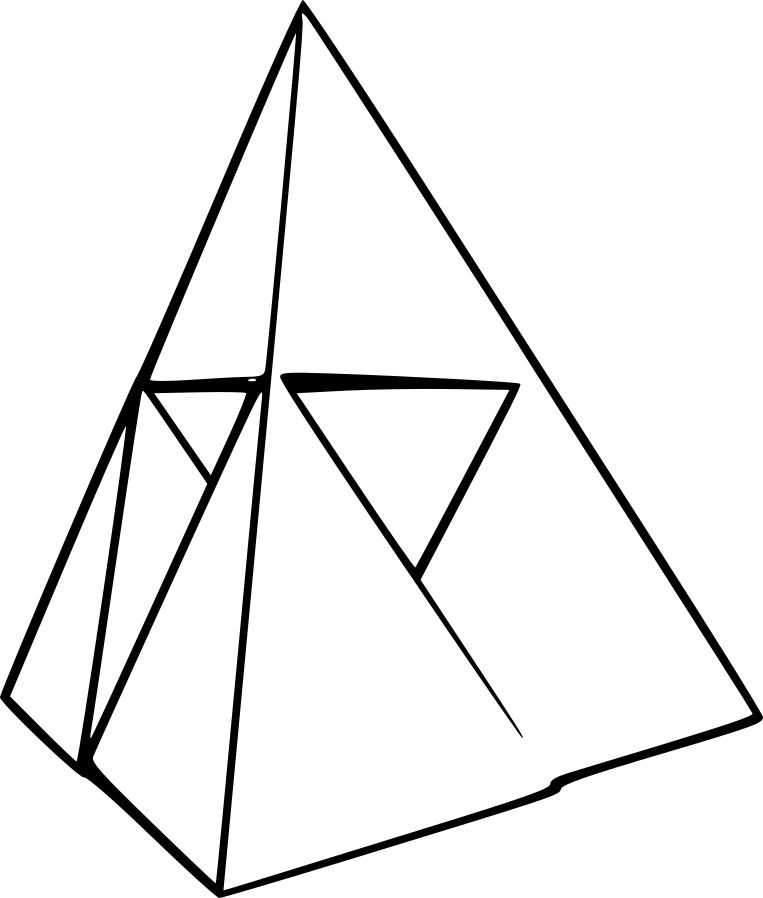
\includegraphics{images/contemplations/contemplation2C.png}
\caption{second Contemplation}
\end{figure}

\subsection{Second Contemplation: Tetrahedral
Fractal}\label{second-contemplation-tetrahedral-fractal}

Sit and look at a free fractal thing in nature while you color this in.
This is symbolizing the fractal nature of truly free things. Trees and
shrubs are all free. Contemplate their fractal nature and their ability
to build this massive structure from the tiny whips of passing carbon
dioxide from the air over many years. Incredible! The tetrahedral
fractal geometry shown in 3d here symbolizes the union of our human
geometry with that of nature.

In this case we flop around on the ground in a more peaceful way, more
slowly, at tai chi speeds even, to try to incorporate the slow pace of
the tree into our thoughts.



\chapter{Principles}
\subsection{Statement of Principles}\label{statement-of-principles}

\begin{itemize}
\tightlist
\item
  All technology should be free
\item
  All people should be free to leave a technical sphere and enter or
  build another one
\item
  All national borders are not legitimate and must be abolished
\item
  The world is magical. The properties we have always called ``magic''
  can be ascribed to all things in the physical world, and these powers
  can be harnessed by the techniques of Trash Magic
\item
  Capitalism cannot and should not be reformed, it should be opposed in
  all places and times until it dies
\item
  The concept of professionalism is harmful to the human condition, it
  poisons the soul, and is evil\\
\item
  The concept of finite number to represent human values is a mind virus
  that must be purged. The infinite exposes deeper truths than the
  finite. These problems go to the deepest level of our mathematical
  thought from arithmetic to the underlying axioms of mathematics
\item
  Morality consists of a set of axioms. An axiom is a unproven statement
  which we take to be true in order to build up a system of thought
  which can guide action. The principles in this list are put forth as
  axioms.
\item
  It is not our role to debate capitalism with its defenders. Every
  possible basic argument for or against capitalism already exists on
  the Internet. Our job is to build a set of moral axioms, a set of
  technical skills and knowledge and build up a practical society from
  that. It is not our job to waste time repeating the same arguments
  with capitalist apologists and time wasters.
\item
  No technology should be made from mass-mined materials
\item
  The sum total of all money that exists in the world is a small
  fraction of what would be needed to compensate the victims of
  capitalism from its crimes(e.g.~slavery and imperialism), thus there
  can be no justice within that system
\item
  Every single word said every single idea ever put forth by an
  economist is a vicious lie. Economics is not a science, and this work
  is rejecting traditional science anyway. It is not our job to argue
  with the economist it is our job to build a better world in which they
  are not welcome.
\item
  The wage system must be abolished
\item
  End work. I am against work in all forms. We must attack the concept
  of work at all levels.
\item
  Technology is personal, as it should be. Relationships between
  technology and the human body are always in mind.
\end{itemize}

\subsection{Design Rules}\label{design-rules}

Engineers who build technology usually use something called ``design
rules'' and ``figures of merit'' as guides for how to build a thing. The
following are the different design rules in which we may deviate from
capitalism to end up with technically different results:

\begin{enumerate}
\def\labelenumi{\arabic{enumi}.}
\tightlist
\item
  The more general solution is always better
\item
  The Most readily available materials are always the first choice to
  use as well as to study
\item
  The most obvious solution is the best, although what is obvious may
  not be obvious
\item
  Self similarity is a desirable property, and by default it will be
  built in for several(but not infinite!) zoom factors to all technical
  systems
\item
  All technology is art, all art is technology
\item
  All technology contains its own data, is linked to itself on the web,
  self documents how to make more, where it came from, where it is going
\item
  Technology is not really deployed until you can create it with zero
  federal reserve debt or consumption of mined or extracted material. To
  deploy a technology is simply to make it and have it get used, and you
  must spend zero money to make that happen. Selling it after that is
  optional, and can be done for workers to get central bank debt
  currency but can also not be, and all parts can float in and out of
  different value circles(more on this later in this work)
\item
  Absolute precision will scale linearly with scale, meaning that we
  might keep just 10\% relative precision at different scales, with
  gross motion at 1 meter with a few cm uncertainty, then a few cm
  motion with a few mm precision, on down to 1 nm motion with 1 angstrom
  precision.\\
\item
  Every piece of technology should be as versatile as possible, with
  clear and easy instructions encoded in it for many uses
\item
  We will not build or work with those who build antipersonnel weapons.
  Drones and other machines are fair game as targets, however
\item
  Every technological component should have the maximum possible number
  of uses, and should be cross referenced with other instances of itself
  so that the user can find out those other uses instantly, and this
  should be true of all the sub-components of a technical artifact
\item
  Every technological artifact and component should tell a personal
  story, connected to users, builders, and artists.
\end{enumerate}

\newpage
\begin{figure}[htbp]
\centering
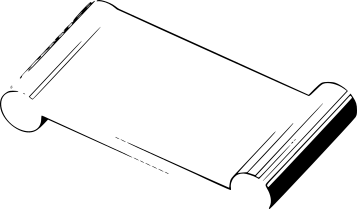
\includegraphics{images/contemplations/contemplation3C.png}
\caption{Third Contemplation}
\end{figure}

\subsection{Third Contemplation:
Scroll}\label{third-contemplation-scroll}

The scroll symbolizes the set of axioms we shall use to build all
things.

This is where we get pumped. You re-read the principles, then put on
get-pumped music and do a series of get-pumped exercises, like fast
punches from horse stance or some axe kicks. Alternate between
coloring/sketching something simple on the scroll with severe activity
of a martial arts nature around the area you are in.



\chapter{What is Trash Magic?}
\section{Chapter 4: What is Trash
Magic?}\label{chapter-4-what-is-trash-magic}

\subsection{Why Trash?}\label{why-trash}

Who owns a dog turd left on the street? Who owns the piles of plastic
bottles that collect in an eddy of an urban stream? Who owns the soot
that collects on the walls of a bus stop? No one. The concept of private
property, which I regard as evil, does not incorporate all things. For
capitalism to function it has to have both ``assets'' and
``liabilities'', which the capitalists associate with opposite signs of
numbers. What if a turd is not a liability or an asset? It does not
exist in the capitalist universe, it is their ultimate trash, of value
to no one, and it is the seed that we must use to create a better world.

\subsection{Why Magic?}\label{why-magic}

Many reasons. First of all, what exactly is magic? It's subjective.
Magic is what, subjectively, gives us a certain feeling of wonder about
the world. I believe that that wonder should be intrinsic to our
technology always, just as we expect it to be with art. Hence the
removal of the artificial separation between art and technology is a
path to what is essentially a form of magic.

Also, the use of this word is very annoying to members of the
technocratic priesthood which this work seeks to undermine. The very
possibility that someone might do something useful and interesting in a
sphere called magical is upsetting to them, because it is clearly not
part of their ``pure'', ``rational'' world. This thus draws a line in
the sand of sorts: on one side is engineering and business and the rest
of the ``rational world'', and our work stands very much on the other
side, where things are a little less sharp and clear and countable.
Hence my statements in the first chapter about Trash Magic being an
artistic movement in this first stage.

\subsection{What is a Trash Witch? What is a Trash
Wizard?}\label{what-is-a-trash-witch-what-is-a-trash-wizard}

Witches and Wizards have for centuries been symbols of humans' ability
to wield various magic powers. I draw on many traditions for this
concept, from pagan lore through Tolkien and Harry Potter. The
traditions built up from fiction, culture, and religions of various
kinds give us a picture to draw on for the archetype of the Trash
Magician. I don't want to use the term ``magician'' too much though
because it can be mistaken for the person who puts on a magic show.
Perhaps that is not all bad, though! The magic show can both teach and
inspire wonder and that is certainly one goal of Trash Magic.

A potential downside of calling us all witches and wizards is that those
can be gendered terms, and that's not what I'm looking for with this new
society. But I will propose for the sake of this work a non gendered
definition of witch and wizard. The person wielding trash magic at any
time is practicing witchery or wizardry if they are doing witch like
magic or wizard like magic.

What?

Well, for example, let's say you're in the woods at night, doing some
hard core potion making and saying something like ``fair is foul and
foul is fair'', and there's a lot of cackling. That's witchery. If
you're in a huge field of rocks swinging your Trash Staff around and
launching lighting bolts at the other rocks, that's wizardry. It doesn't
matter what gender the practitioner may or may not have--if you are
wizarding you're a wizard, if you're witching you're a witch. At least
for the moment. Mostly trash magicians have both Trash Wizard and Trash
Witch natures, and most magics we practice will use both as well.

But I have still only loosely defined this way of being. The Trash witch
is someone who believes in a world where we both have a element of
adventure and mystery in our lives and where we have the advantages of
what we now call ``modern technology''. We believe that this magic
should be available freely to everyone in the world, and that everyone
in the world should have the freedom to wield this and modify it as they
see fit, and use or not use whatever magic they need or don't need.

Trash Wizards and Trash Witches use the laws of physics and the methods
of applied physics as a form of magic. We teach that magic to others,
and spread both the serious scholarship of Trash Magic and the basic
practical skills needed to give the magic to all.

All our teaching and building is free. Free, meaning outside the money
system and capitalist economy. But also free meaning people have total
freedom to take this and duplicate it and modify it and make it truly
their own. A love of pure science demos is a core value of the Trash
Wizard or Witch.

Another goal is independence. A group of just Trash Witches should for
example be able to live on their own, with a good quality of life. Maybe
dozens of Wizards or dozens of Witches can easily form tribes to build
and scavenge and do adventures and art. But also tribes can form
super-tribes which merge to build truly large works. The only way giant
social structures can be optional and not control us all is for us to be
able to live freely with just a few people. The magic we plan to wield
here is designed to give people that power.

\begin{figure}[htbp]
\centering
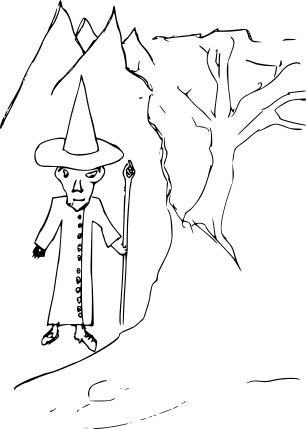
\includegraphics{images/wizardcartoon.png}
\caption{Wizard by the creek}
\end{figure}

We also strive to amuse. You don't want to learn about magnetic fields
just for the hell of it or just because they're useful. You can see from
us that they're actually magical! Magical enough that a show put on with
magnetic fields or electric fields is very much worth watching. In fact,
one of the most popular shows in most science museums is the electric
field demonstrations with giant lighting machines.

So a Trash Magician uses a combination of Wizardry and Witchery to amuse
and provide for people with Trash of the world. Trash is generally stuff
that is not only free but infinitely free. Not only can you go find one
or two or 10,000 of a thing, you know that later you can go back and do
that again as many times as you want. This is true with flowing water
from spring snow runoff or from tides or drainage of some large rainy
area. It's true of winds that always blow, of the sun, of sand and dirt
and rocks. It's true of sticks shed by the lower sections of pine trees.
And it's true of the plastic bottles thrown away by capitalist society.

A society of free stuff is not one with ``zero cost''. It's one where
cost is infinite but value is also infinite. We are moving to a value
system that works mostly with infinities. That is part of what makes
Trash Magic actually magical. And if you're a Trash Witch or Wizard,
that's your stuff! You wield the magic that moves the trash around!

In addition to Trash Wizardry and Witchery one might be a Trash Daemon
or Trash Imp. Trash Goblins can have a place in our community but not
Trolls.

Trash Wizards are always there for everyone. We welcome the refugees of
capitalism and it's evil twin, war. WE do not recognize the validity of
borders and are here to help subvert them as needed to help the down
trodden.

\subsection{Alchemy, Chemistry and Art}\label{alchemy-chemistry-and-art}

Part of the narrative we learn when we study chemistry in school is that
of the failure of alchemy to accurately describe the elements. We learn
that these primitive pre-chemists thought of the elements as being
earth, air, fire and water, rather than the array of chemical elements
we know in today's periodic table. The \emph{real} elements are divided
up based on our supposedly superior modern understanding that atoms are
the basis of all matter.

I dispute none of basic science we all learned in school in terms of
atomic structure, this manifesto is not quite that kooky. What I do
dispute is how information is organized in our minds and in our equation
system. Consider an element like oxygen. We know that a lot of oxygen in
the world around us is in the form of two atoms together, as a gas which
makes up about one fifth of the air around us. We also know that all
water has one oxygen atom(along with two hydrogens), and so all the
water in our world has oxygen. Fire is pretty much always a rapid
chemical reaction involving oxygen, so we also know that all the flames
we see in our world on Earth are partly made from a form of oxygen.
Finally, the one of the most common minerals on our planet is the
relatively inert silicon dioxide that makes up most sand as well as many
other minerals. The melting point of this solid is well over one
thousand degrees.

Now, while I would never deny that it's useful to say all these things
have oxygen, or to understand what that means, is that really the most
pertinent quality they all have? To the alchemist sand is ``earth'',
fire is fire, water is water, and air is air. Four elements, which we
deal with very differently in all possible ways. We look at that and say
it's ``wrong'' because the knowledge of what atoms make up these things
is somehow more ``fundamental'' supposedly. But what if we didn't
organize things that way, even though we understand how atoms work? What
if we still recognized that earth, air, water, and fire as elements,
which just happen to be also made up of atoms? This world view would
have the same facts as the one we hold today, just with their order
re-arranged.

Ideally what I seek from this project is to remove these kinds of
hierarchies altogether. I don't want to say that alchemy is ``right''
and chemistry is ``wrong'', what I object to is the basic notion of
right and wrong here. It's based on the notion of our ideas having some
kind of objective other reality beyond that of the world we live in. I
think this kind of ordering of ideas is one of the ways we've held
ourselves back in science due to ideology.

We need to stop banishing things like spells and elementals and potions
from ``real'' science just because of cultural values. A drug is a magic
potion, what else would it be? Prove it isn't! A program on the firmware
of a robot is a magic spell. Prove it isn't! And every artist knows art
is magic. The only way we have denied that in science is by simply
saying we're better than art on the ladder of ``reality''. This has,
again, held us all back. It's led to a century of inaccessible art and
incomprehensible science. We need to reunite the strands of alchemy,
magic, art, and science.

\subsection{Symbology}\label{symbology}

Where to trash magic artists get our symbols? From the natural world,
from geometry, from anarchist iconography, and from religious art. We
also seek to replicate, but softened by the influence of the natural
world, the design aesthetics of 20th century industry. This will be
almost a parody or a three dimensional rhyme of sorts, not so much to
bring out the function of the industrial thing but to remind us of its
form to make us think of where our trash comes from and what we are
replacing.

Note that when I say religious art, this is very broad, since much of
art through the ages has always been inspired by whatever the artist
viewed religion to mean. Religion is our deepest held beliefs which form
our world view outside of that which can be proven. Art at its best
tries to express what that means, and is often deeply religious, but
takes very different forms due to the diversity of religious beliefs. In
particular, however, trash magic will lean toward the ``occult'' from
various Western traditions. Due to the author's non-indigenous Western
background, I want to avoid appropriating cultural traditions of which
I'm not a part. And I feel like one way to do this is to focus on
``pagan'' traditions of various kinds, as well as occult Jewish and
Christian art.

The anarchist symbology will include the black wild cat used by the IWW
and other anarchists, as well as various permutations of the circle A.
The following image combines the black cat with the form of the magnetic
field from a tiny magnet, symbolizing one of the forces which we will
harness in Trash Magic.

\begin{figure}[htbp]
\centering
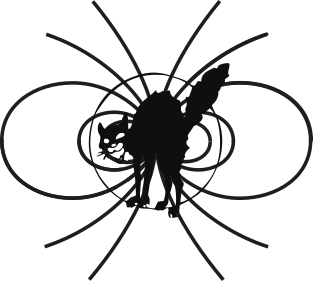
\includegraphics{images/cat3.png}
\caption{Wildcat in the field}
\end{figure}

\begin{figure}[htbp]
\centering
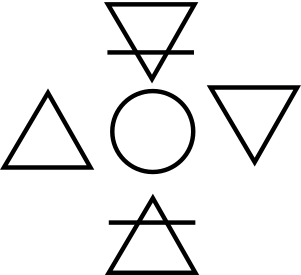
\includegraphics{images/elements.png}
\caption{Elements}
\end{figure}

Some electrical symbols will also be incorporated, partly since many
things we will make involve building electrical circuits, and building
those symbols into the art makes things self-documenting. While these
form a useful function in helping to make a thing free by documenting
how it's put together, they should never abandon form for function:
circuit documentation should be a work of art as much as a document.

Secret symbolism in occult art at UAA library: BF1623.S9 G45 1987

Art and the occult, UAA library: N8222.M3.S38 1975

\subsection{Capitalisms Unwanted: a Human
Treasure}\label{capitalisms-unwanted-a-human-treasure}

What is a Trash Wizard?

What do we do?

What is best in life, redux

How the trash wizards teach the world our methods

What kind of world we build

Many wizardries, many paths

How does the value circle work?

how do trash wizards spread the value circles?

Specific examples of value circle use: manufacturing, food, robots,
coffee, R\&D, art

Many technical details on trash wizard sticks, how they're used,
designs, plans, images, examples, etc etc. on the sticks.

Use of sticks with cars, computers, phones

using the stick to replace the smart phone eventually

\subsection{What Does the Trash Wizard Stick do and
have?}\label{what-does-the-trash-wizard-stick-do-and-have}

\begin{enumerate}
\def\labelenumi{\arabic{enumi}.}
\tightlist
\item
  built in measuring stick in SI and English
\item
  build in measure tool for AWG of wires
\item
  LRC meter that reads out on phone
\item
  conversion to robot mode where it drives itself around
\item
  convenient single shoulder strap for comfortable wear like a bike
  messenger pack
\item
  random flash sticks which store MP3's of music ripped from youtube on
  the pi, controlled by the smart phone, and then replayed later
\item
  speaker built from our technology, reading flash drives out with the
  pi zero
\item
  pi zero
\item
  High voltage storage caps(detachable)
\item
  medium voltage storage caps(detachable)
\item
  super cap(detacheable)
\item
  LiPo Battery(detacheable)
\item
  direct wire connect silicone and copper switch board for power with
  fail safes of various kinds
\item
  screen for pi zero to read out a special dumb ass bat phone
\item
  measure nonlinear voltage response to impulse of various random blobs
  you find around
\item
  can harvest energy using a built in magnet and coil setup
\item
  water pump always available
\item
  trash wizard app for phone is set up for physics, interfaces with
  existing physics packages
\end{enumerate}

\subsection{Trash wizard multi tool}\label{trash-wizard-multi-tool}

I want the trash wizard multi tool to be able to measure inductance
easily. How to do that? I want the L/R time of something to be long
enough to see something on the arduino ADC. But what R? If L is 0.001 H
and R is 1 ohm, L/R is 1 ms. Perhaps a 1 ohm shunt resistor somewhere.

Or maybe I want to measure the reverse EMF from changing the current
quickly through the coil. V = L dI/dT. For a 1k series resistor driven
by 3 V we have 3 mA of current. If that can turn off or on in a few
microseconds, it should be possible to induce a good fraction of a volt.
But given that the sign will reverse, having this go to ground would be
a problem for the ADCs on the arduino. So what I want is a 500 ohm
resistor going from the DAC to a node between two 500 ohm resistors in
series making a voltage divider between 0 V and 3.3 V. that middle node
then goes to the ADC and pulses should be visible. This I will not
proceed to build and test.

\subsection{Free Phones of the Future}\label{free-phones-of-the-future}

One of the many idiotic things capitalists say to shut up their critics
is to point out that capitalism is the source of the smart phones that
anti capitalists inevitably use. These devices are indeed amazing, and
are no longer luxury items by any means. On the contrary, they are very
much a survival tool used by the oppressed classes now, and it's very
dangerous to ignore that role this technology plays. But what aspect of
them is so great? The social networking. That's always what you need:
access to the web, various messaging systems, and various commercial
things like Uber and Lyft.

Does that really need to be a computer? A truly free phone would be a
pure communication tool that communicates in a distributed way like fido
net of old. the sole purpose of the hardware would be to communicate
images, sounds, text, and to decide where those should go. That's it.
What the hell do you need a computer for? Mostly so that The Man can spy
on you and figure out how to sell you shit you don't need, and force you
to constantly throw more federal reserve debt back into the machine for
more advanced machines to get more indoctrination to continue the cycle.

It's all bullshit! Don't be fooled by the dominance of the computer
technology into believing that's inevitable. It's not. We can get orders
of magnitude more benefit from peer to peer networks than we do today as
slaves to the military industrial machine if these phones were all free
like freedom, linked up on free hardware all the way. This can actually
be the basic informational skeleton of the value circles.

I believe that the hardware can be re worked from the ground up based on
our approach to applied electromagnetism to get something with totally
new fab. But in the mean time, given that that is a lengthy applied
physics research project, what can we do? My answer is to watch closely
everything that has anything to do with Raspberry Pi and other
``internet of things'' projects in the open hardware domain. I say
``open hardware'' here and not free hardware, because it's not free
according to my strict definition: it relies on mine- driven fab and
capitalism, and there is IP in the supply chain(and some other
problems). But it's way better in terms of open and free than the whole
android/apple ecosystem.

as seen here: https://www.adafruit.com/products/2885
(https://www.adafruit.com/products/2885) The pi zero sells for 5
dollars! And it's free like freedom as far as the software goes, as I
understand it. The problem of course is that it's not what you'd call a
product still. You need to buy a screen separately, and a battery, and
some other odds and ends, and then put a package together, get all the
software working, etc. It's not trivial. Not insanely hard, but not
trivial and also not really as usable as a apple or android. But surely
this could change? If people want to work within the system of existing
``tech'' a fantastic place to focus efforts would be making this
technology closer to truly free. This will be a combination of figuring
out sourcing logistics on the hardware, making the software closer to
what a phone user expects, and writing new software to make more free
infrastructure that runs on the free hardware. If a truly free platform
were to allow for the kind of peer to peer labor and goods sharing that
for profit platforms now have, capitalism might just collapse overnight
as people spontaneously are able to work and do things by communicating
freely.

Don't like the phone but like ``tech''? make a free phone. It will
happen one way or the other, but the more ways it happens the better for
everyone.

\subsection{How to Build the Team to build the
Technology}\label{how-to-build-the-team-to-build-the-technology}

I'm clearly not going to build all the things I'm describing here. And
even the things I do build, I hope to have what I build be a
insignificant fraction of the total number of units produced in the
future. How to recruit? Who to recruit? Where will they work? I've been
contemplating these questions, and I see several ways to proceed.

Largely the various ways forward will involve decisions about where to
be on the spectrum of working inside the system vs.~outside. Some
choices will involve getting very conventional, and I fear they will end
up being coopted by the existing system. One of those would be to
structure the way ARPA was in ins heyday. Many top academic, corporate,
and government research labs could receive targeted funds to work on
problems, where the funds come from various donations and military
applied science grant money. The work would then be done by the usual
suspects: grad students, post docs, and various staff researchers inside
the current system. I think the biggest danger here is that the
developed technologies will not be free in the real sense because it's
so hard for a expensive R\&D lab to ever build a thing that's not based
on expensive equipment.

Another way forward is to focus on commercial applications in the old
economy. One could for instance build a very reliable and cheap water
pump, and build a rapidly growing for-profit company on that which funds
R\&D to free technology through its profits. This is, I think, the worst
of all possible choices. Capitalism poisons everything it touches. And I
think the way I'm going to define capitalism for the purpose of this
work is ``the belief that value can be measured using numbers''. It's
that simple. Any kind of money or equivalent value unit that can be
counted is the poison we all know from our capitalist nightmare, and
that's what I'm going to focus on purging from the technological supply
chain.

At the other end of the spectrum, one imagines seizing a abandoned
factory building and building the R\&D infrastructure up from scratch in
a squat environment. I predict that going too far down this path ends
with the usual endless war with cops and landlords that always happens
when good people try to use land without the System. Even if you imagine
buying the land so that there are no direct legal challenges, cops and
landlords will be an ever-present problem, as will generating enough
federal reserve debt to keep the bastards off our backs. A lot of time
will have to be spent on just keeping the site running.

Seizing land and building up the means of production makes sense when
you have a working technology that can be instantly deployed and then
also broken down and moved later when you need to move. But before the
technology is mature, it makes sense to be completely distributed
geographically. Also, for this project to work as I want it too, we need
strong cooperation between the developing world and the developed world,
and between diverse people living on land that has different types of
local resources available from whatever their local trash streams are,
as well as the very diverse energy considerations, and the diverse
cultural considerations which should be considered early not later.

How does this distributed system work? I believe part of it involves the
structure of the actual book document. I don't feel that the Jupiter
notebooks are quite where I want them yet, but they're close, and I
think that the structure will be based on software that comes out of
that basic structure. Users will make modules to solve various technical
problems, as well as post new ones, and they'll all be integrated into
the combined book. This is, in many ways, what the open source software
people do using their git hub bullshit. I think git up is a giant
festering piece of shit, however, and loathe most software communities,
so this is a tricky game. Somehow the innovations from that world should
be used without poisoning the whole project and creating yet another
tech bro shit head club.

One way I want to differentiate from a lot of computer software bullshit
is by having a coherent narrative. Something that drives me crazy about
their culture is that things are so distributed that you can't actually
figure out where to start. It's not just that there are forks, it's that
there are many forks all the time for everything and everyone is a giant
dick about all of it. I'm not above simply banning anyone with any tech
company affiliations from contributing to the main document.

This is a book. A book is a finite thing. As time goes on content will
be added, but other content will also be deleted. It will all be
archived, but if someone wants to they can approach from zero, start at
the beginning, and have a coherent narrative to follow as they build up
to actually having the ability to use the technology themselves. There
will be various versions to account for many human languages as well as
some various tracks that might exist, but all of the parallel versions
and tracks must be self contained and linear(or at least with the option
of treating them as linear). I need to keep a very close eye on how
things progress with the various jupiter like things out there, because
it's moving fast. It all has to work on a free trash wizard stick, but
that should be fine with the HTML5 stuff that everything now runs on
inside a browser. Is there a simple way to go back and forth between
jupiter notebooks and a fully compiled .pdf in book format? Surely there
is, and if not, it should be some combination of existing scripts
chained together.

My job as initial author is to create well posed problems in the first
draft of the book, and to make it appealing for people to contribute
solutions to those problems. This will be extremely hard to get right on
a first pass, and part of getting this whole thing to work will involve
shifting that format over time. When things are really working, the R\&D
will be all done in the value circle economy, where people are
constantly creating that form of value as they do R\&D. This has the
potential to be a very hard chicken-and-egg problem: the book needs a
lot of work in order to have value circles work, but without value
circles people can't work on it effectively. That's why this all starts
with me working alone in my underwear at home. And remains that way for
a while. Because I need to first have the system working with me as the
only user, then me and some close associates, then a few ``followers''
who just build kits, and then, when that team has worked for a few
years, more people can ease their way into the system to grow it. Of
course as the serial/parallel global crises of capitalist disaster
accelerate, we may find that things grow explosively instead. If that
happens it happens, but I will plan for something that is built much
more carefully.

This blog post was going to go into a list if the types of experts
needed to get the various jobs done, but on looking where it ended up
going that looks more and more like a useless exercise at this time.
I'll build up the vision of what should get built, build my own parts of
that technology and distribute them, and then a sort of chemical
potential will form which brings in the right experts. It's dangerous to
specify exact professional qualifications too early, as it will end up
losing out on some opportunities to bring in talent outside the
organized technical professions, which creates lots of biases in class,
race, nationality, age, etc. It's much better to pose problems clearly
with no jargon, in as many ways as possible and just see who turns up
with a solution.

\subsection{Skeletron: The Wooden Bones of
Art}\label{skeletron-the-wooden-bones-of-art}

Skeletron is the system that makes the bones of Trash Magic artifacts.
Skeletron is simply a way to modify things found in your environment to
make them play together well with Trash Magic. Primarily this means
gathering sticks, shaving them to be flat on one or more sides and
removing the bark, and drilling holes in them. Quarter inch holes spaced
about one inch along the line of the sticks is the most basic component
of Skeletron. This can be used to do many things, and as more people
build it and use it and modify it, it will become increasingly versatile
and free.

With a universal wood framing system we can build up many different
human sized structures. This can be used to make various shelters,
although to do this we will add plastics to the system, using methods of
hand plastic welding detailed in the last chapter of this volume. With
the ability to make wood skeletons with plastic skins we can make
waterproof structures on land as well as waterproof boat structures and
amphibious artifacts of various kinds. The combination of wood and
plastic in a modular and modifiable way also can be the basis of all the
other industrial constructions to be described in this work.

The fasteners to hold the sticks together are all quarter twenty, or one
quarter inch outer diameter threads with 20 threads per inch, a very
common standard in the US. In Metric countries, the equivalent would be
about M6. The M6 and the quarter inch threads are not compatible, but
the hole sizes should be, especially if you drill them out big enough to
have some extra space around the bolts. Bolts and nuts can be stainless
steel if you want to buy some, or melted plastic can be used to make
plastic bolts and nuts and wrenches from bottle caps or other similar
plastics.

In addition to making large sticks with many holes in them and welded
plastic sheets for water tight construction, we have a system for
building electronics directly into the sticks. This involves some
soldering techniques detailed in the last chapter of this volume as
well, as well as the plastic welding techniques to fix in place, strain
relieve and protect the circuits as needed.

A drill is needed for this work to cut the quarter inch holes for the
main Skeletron sticks as well as to make smaller holes for various wires
and components for the electrical circuits. While it can be easy with
Grid access to use a simple electric power drill, the ideal Trash Magic
industrial production will involve a direct drive drill driven by
flowing water.

\newpage
\begin{figure}[htbp]
\centering
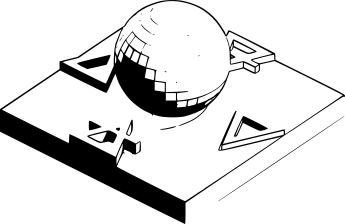
\includegraphics{images/contemplations/contemplation4C.png}
\caption{Fourth Contemplation}
\end{figure}

\subsection{Fourth Contemplation: Elements of
Alchemy}\label{fourth-contemplation-elements-of-alchemy}

Having gotten a hard awesome workout in the previous Contemplation, this
one is more contemplative, and you assume a meditative physical posture.
Turn your mind inward to your body and see all five of the elements
here: water in most of our bodies, earth in our bones, air you breathe
in, fire in the use of oxygen from air to liberate chemical energy from
food which then leads to flow of ions through the water. These five
elements are in your body everywhere! See them. For specific details on
the alchemy symbols, look them up--it's a vast subject.


\chapter{Universities}
\subsection{Universities: Visions of
Utopia}\label{universities-visions-of-utopia}

If the university campus lived up to its potential it could be a true
paradise: essentially a giant garden filled with buildings for studying
and creating knowledge. Amazing! They are usually situated on some of
the best land to be found anywhere, have great access to everything
needed in life, and have dense urban style housing in a pastoral
environment which allows for a simple, car free life.

University campuses are often physically spectacular. They often have
some of the greatest examples of art and architecture of available both
used in their construction and lovingly maintained for in some cases
hundreds of years. It is typical for them to have wooded areas owned by
the university, as well as often running water and in many cases access
to very large bodies of water. University campuses are often more self
contained than most institutions, creating their own power and managing
their own utilities, and having a fair amount of autonomy from local
government.

\subsection{Brief History of the
University}\label{brief-history-of-the-university}

Where did the universities come from?

University as a challenge to secular corporate rule.

Looking up sources at UAA library.

The universities of Europe, 1100-1914 : a history is at LA627.R82 1984

This needs extensive library research.

\subsection{Undergraduate Education: Broken
Promises}\label{undergraduate-education-broken-promises}

The college education has become a key element in the great lie of the
American middle class dream. It is also a major factor in the older
generation destroying the opportunities they had for the younger
generation.

College has become just another capitalist cartel, exploiting the hopes
of young people in exchange for a life of debt servitude. Young people
are still told by their elders that a college education is needed to
enter the middle class, which is supposed to be a good thing. They're
told that the price is justified by long term earnings. Then they're
sent off to live in a party resort for 5 years where they shuffle
through a series of pointless and irrelevant classes, and wind up with a
bill of many tens of thousands of dollars(this is primarily an American
problem, but the neoliberals will bring it to your country soon enough
if they're not crushed at the global level).

And what do we learn there? Theory! Propaganda! How to write papers no
one will read about stuff no one cares about. 100 year old science. At
this point defenders of the System start howling about ``pure
knowledge'', by which they mean theory over ``applied knowledge'', by
which they mean actual knowledge about how the world works. Theory is a
virus, a disease, and a religion, and it has no place here.

What should we learn? Same subjects, but useful. Why can't biology
majors make drugs? Why can't physics majors build a flying drone? Why
can't chemistry majors build a water desalination plant? Many subjects
should, I think, be totally eliminated, as they have no real value, such
as economics and computer ``science''.

\subsection{Science Grad School: The Ponzi
Scheme}\label{science-grad-school-the-ponzi-scheme}

You don't have to go to graduate school to see how much it resembles a
pyramid scam. Suppose any one professor has about five graduate students
at a time, each of whom takes about five years to graduate with a PhD.
If a professor does this for 30 years, they will create on average one
PhD per year or 30 PhD's total. Now suppose all those PhD's find jobs
similar to what their advisor has. This is possible only if the size of
the field increases by 30 times in 30 years. Very crudely this
corresponds to about 12\% per year. Given the expansion of the physical
sciences and their satellites in the years during and directly after
World War II, building a scheme like this in those years actually made
some sense. However, those days are decades behind us, and now as
research budgets shrink and schools, companies, and government agencies
are systematically destroyed by politics, this math looks much more like
a pyramid scam than a response to society's needs.

As a grad student you will \emph{probably} never get the job you're
supposedly being trained for. But you will dedicate 5-7 years of your
life to helping someone who \emph{did} get that job to continue to climb
the academic ladder. The people at the bottom of the academic pyramid
spend their lives working to help the people at the top, and then are
mostly cast aside.

The tenure clock then puts yet another opportunity for exploitation in
the career path, making yet another way for people now well into middle
age to work long hours for more years to build up an academy that they
might then be cast out of.

\subsection{Hollowing Out of the
Academy}\label{hollowing-out-of-the-academy}

There are many factors that have contributed to the downfall of the
university system over the last few years. I would argue that since
Ronald Reagan was elected president of the United States in 1980 there
has been a coordinated ideological war against all culture that might
exist outside of the profit system, and that universities have felt the
brunt of this particularly hard.

A robust, healthy, independent, and publicly supported university system
could provide a real balance against mainstream corporate power if it
existed. It is therefore strategically important for the lords of global
corporate rule that they be as controlled as possible by corporations
and the central government so that they cannot exercise a check on those
forms of power.

\subsection{Intellectual Property}\label{intellectual-property}

Intellectual property deserves its own section here because it has been
so corrosive to the culture of the academy in so many ways. This
manifesto is opposed to all forms of private property, and particularly
intellectual property, but the patenting and copyrighting of work done
in universities is particularly evil.

It is now standard practice for public tax money to be spent to create
knowledge which then goes into papers behind a paywall protected by
brutal copyright enforcement and into patented or even trade secret
knowledge. If the rule of law actually meant anything this would clearly
constitute a criminal theft from the public. The fact that this is
\emph{not} considered a criminal act is in fact a major indication of
the evil nature of the capitalists' so-called ``rule of law''.

\subsection{Potential Paradises}\label{potential-paradises}

\subsection{University Occupations, Phase
2}\label{university-occupations-phase-2}

Any history of any radical movement will inevitably involve student
occupations. Students typically take over some space on campus, keep the
land from the cops, and carry out various protest actions or teach ins
over some number of days or maybe weeks. In some cases they stand down
after actually getting some demands met by the administration.

\subsection{Case Study: MIT and
Harvard}\label{case-study-mit-and-harvard}

MIT(Massachusetts Institute of Technology) and Harvard share a strategic
position along a tidal waterway, the Charles River. I will look at both
of them here and point to how an insurrection in either institution
could grow out into that river and have lasting impact after the initial
event.

And what of the Charles River?

\url{https://www.worldcat.org/title/charles/oclc/990111} looks like a
good reference, can be found in denver libraries and dc, but not
anchorage.

\begin{itemize}
\tightlist
\item
  How much land owned?
\item
  How much is arable?
\item
  How much is already zoned for ag?
\item
  What water resrouces are there?
\item
  number of staff, students, alumni, faculty
\item
  How many people could Yale support?
\item
  Holdings outside New Haven
\item
  Yale Singapore
\item
  Repurposing the Endowment, total divestment from capitalism
\item
  political and legal process of re-writing the charter of the school,
  changing governance
\end{itemize}

yale history:
https://www.worldcat.org/title/yale-university/oclc/40331263\&referer=brief\_results

yale land holdings:

\url{http://sustainability.yale.edu/planning-progress/areas-focus/landscape}

charter:
\url{http://www.yale.edu/sites/default/files/files/University-Charter.pdf}

\subsection{Case Study: University of
Paris(Sorbonne)}\label{case-study-university-of-parissorbonne}

\begin{figure}[htbp]
\centering
\includegraphics{images/Sorbonne.png}
\caption{The Sorbonne}
\end{figure}

\url{https://en.wikipedia.org/wiki/University_of_Paris}

\url{https://en.wikipedia.org/wiki/University_of_Paris_strike_of_1229}

\subsection{Case Study: Roosevelt
Island}\label{case-study-roosevelt-island}

Need to go look up reports on this project, detailed maps of the island,
go see it and investigate, take pictures.

\url{https://en.wikipedia.org/wiki/Cornell_Tech}

\begin{figure}[htbp]
\centering
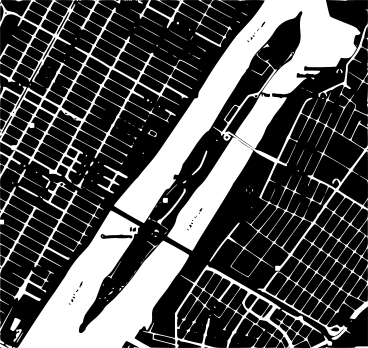
\includegraphics{images/roosevelt.png}
\caption{Map showing location of Roosevelt Island in the East River,
between Manhattan island and the Eastern boroughs of New York City.}
\end{figure}

\subsubsection{this chapter should have a section with a detailed
example}\label{this-chapter-should-have-a-section-with-a-detailed-example}

maps, tables, really dig in and figure out the strategy and tactics that
could be used, maybe have multiple examples, small liberal arts, huge
public school, elite private school, community college in a big city

\subsubsection{The Universities are a
Disaster}\label{the-universities-are-a-disaster}

\begin{itemize}
\item
  Academia as pyramid scam
\item
  Academia as tool of the military industrial State
\item
  Academia as a marketing tool for the banking cartel
\item
  Academia: where ideas go to die
\item
  Academia: it was here before capitalism and it will be here after
\item
  Has traditionally been a part of various religions and patriarchal
  systems connected with them
\end{itemize}

IP is key to how bad it is, academia after the re-occupation of the
campus all property will be banned from campus.

\subsubsection{But they're really useful to
us}\label{but-theyre-really-useful-to-us}

Back to basics: knowledge, teaching, philosophy, technology, culture,
books, land, food and energy

Universities must be Occupied and declared independent

This should be across disciplines and outside of the capitalist class
system, bringing in workers, locals, students, teachers, researchers and
everyone else involved. Seize the legal control of the corporation that
is the University, and you will have a power that States must respect.

Taking universities over can be a huge international beach head that
goes around all national borders.

Important reference:

Universities, Inc.

call number: 338.43378 WASHBURN

DPL description:

``Our federal and state tax dollars are going to fund higher education.
If corporations kick in a little more, should they be able to dictate
the research or own the discoveries?During the past two decades,
commercial forces have quietly transformed virtually every aspect of
academic life. Corporate funding of universities is growing and the
money comes with strings attached. In return for this funding,
universities and professors are acting more and more like for-profit
patent factories: university funds are shifting from the humanities and
the less profitable science departments into research labs, and the
skill of teaching is valued less and less. Slowly but surely,
universities are abandoning their traditional role as disinterested
sources of education, alternative perspectives, and wisdom.This growing
influence of corporations over universities affects more than just
today's college students (and their parents); it compromises the future
of all those whose careers depend on a university education, and all
those who will be employed, governed, or taught by the products of
American universities.''

\newpage
\begin{figure}[htbp]
\centering
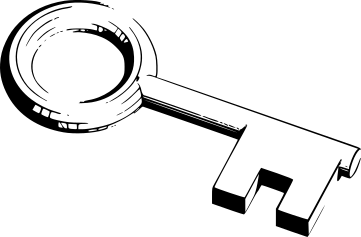
\includegraphics{images/contemplations/contemplation5C.png}
\caption{Fifth Contemplation}
\end{figure}

\subsection{Fifth Contemplation: Key of
Knowledge}\label{fifth-contemplation-key-of-knowledge}

This is an adventure! Take your coloring book out to the local college
campus and walk the land, stopping to color in random bits of the key
while looking around and taking it all in. What could you build here?


\chapter{Rumbles of Robots}
\subsection{Robots!}\label{robots}

Robots! The word is loaded with both promise and peril. We dream of
robots that do all tedious labor, freeing humanity from it, as well as
of robots that might take over and kill us all(fiction seems to favor
the latter).

I also believe robots can be transformative, although I think we should
look at much of the hype from today's ``tech'' companies with many
grains of salt. Self driving cars and autonomous battle robots have
mostly turned out to be worthless hype machines useful for making
Silicon Valley hucksters rich and not for much else.

Here I will look at some of the robots I think we should build with
Trash Magic which can make a better world for caring for one another and
having adventures, which is what this book is all about.

\subsection{A Rumble of Robots}\label{a-rumble-of-robots}

The collective noun for robots is ``a rumble of robots.'' I'm not sure
where I heard this, I think one of my friends may have made it up, but
it's so perfect it's too good not to use. So I want to talk about
rumbles of robots. In particular the difference between robots used for
consumption and for production.

Amazon is in the process of building robot based infrastructure for
delivery. This is fundamentally a consumption driven project. The main
initial figure of merit in the growth of their network will be coverage:
the more potential consumers are covered, the better. This will mean
that it is optimal for robots to be as far as possible from other
robots. But how does this picture change for production?

Rumbles of robots are very common on the production side of things.
Those who produce cars and computers and the like often have rumbles of
robots, with humans just as technicians who run the machines. Much like
a cow hand or shepherd, I think there should be a name for those who
herd rumbles of robots: rumbler. So the trash wizard is also a rumbler.
And the trash wizard stick is like the shepherd's crook: a device that
controls a network that consists of your rumble of robots.

That is what seizing the means of production is really all about. It's
not about seizing an existing factory, which will be based on existing
methods, or about building a primitive system that can't compete. It's
about building rumbles of robots which can reproduce themselves by
harvesting free materials to make more, and then rumbling them around to
build what else you need.

Key elements of the trash wizards robot rumble are mobility and
versatility. They will run off of locally harvested energy, and be
programmed to gather energy as needed as well as materials. They should
scale in that the robots you need for a 10 bot rumble are not so
different from a single roninbot or a 1000 bot rumble. They should be
able to reproduce from found materials and forage for those materials
with some simple guidance from the rumbler. That is the plan.

\subsection{Robots with different times scales, centuries of work, or
hours of
lifetime}\label{robots-with-different-times-scales-centuries-of-work-or-hours-of-lifetime}

Something that I think needs to be investigated in robot design is time
scale. Capitalists like a certain time scale--the shorter the better.
But without capitalism and its obsession with short term growth and
profits we can set times scales on hundreds of years or even longer in
some cases. Suppose an area of land is contaminated with plutonium or
some other radioactive heavy metal. It might be there for many thousands
of years, making the land uninhabitable. Thousands of years, but not
forever, and plutonium has uses even in a peaceful society without
rules. Why not clean it up?

Perhaps the robots that clean plutonium will grow their own biofuel to
get energy from the sun and slowly pick their way across the land,
working with cyborg worms and fungi to dig up the atoms and move them
together and out of the water table. How many processes of atomic or
molecular transport open up when we allow a process to take thousands of
years? Many. I'm sure capitalists already use the term ``geological
engineering'' but I would say that to truly apply that term, you should
be carrying out a technical/artistic endeavor which takes place on a
geological time scale. That means it has to be \emph{very} easy for
future people to understand, maintain and repair. It also has to
anticipate future geological changes, including catastrophic ones like a
volcano that destroyed all life on earth for a billion years. And it
should have time horizons that stretch well into the 10's of millions of
years. What's your hurry! If we were not all hounded by debt to
capitalists we could take time to really work on hard things like
plutonium cleanup one atom at a time.

\subsection{Earth Robots}\label{earth-robots}

The octahedral ball drone is a octahedron made of three intersecting
sticks, with a flexible joint. Simple mechanical motions of the tips of
the ball-like shape cause it to roll across the landscape with a slight
hopping or walking aspect that makes it able to deal with very rough
terrain.

Rolling ball robots can be used for all sorts of long slow land cleaning
processes. Rather than try to maximize battery life, they will use
capacitors to store energy, and recharge the capacitors from ambient
energy. For a rumble of jacks in the prairie, the obvious source of
power is the wind. Ideally, the wind will be used to create energy which
will immediately go into directed propulsion. This might be slow since
it depends on gusts, but it can go on forever, so slowness becomes ok.
This is technology that you would deploy to spend 1000 years cleaning up
a sacrifice zone, where you want no outside energy or materials to be
needed at all and for the rumble to keep doing its work for hundreds of
years. Also, obviously, clearing of mine fields is a immediate
application. A rumble of tire-sized octahedra could potentially roll
themselves at 10's of miles per hour, keeping up with a car or truck and
making it possible for the rumble to proceed in a mob ahead of a motor
vehicle, taking out IED's in real time. The rumble could end up in a
convoy geometry, stretched out over the length of the road, doing recon
ahead and tracking behind to see what's happening after a convoy passes.
In these applications it probably makes sense for the source of power to
be the trucks or cars in the human/freight convoy, with individuals in
the rumble cycling through the charging station and back out into the
rumble.

These are a great tool for agriculture, or even just gathering. A
gathering rumble could go out and gather roots and berries from the
countryside in a quasi-cultivated area. These roving balls could be
picking up and dropping seeds as they go, mapping where all the useful
plants are, and also harvesting as they go, taking wind sun and water as
energy sources as needed, then spending energy when it's available to do
the work.

Rolling robots with windmills: they roll, then gather wind electricity
into a capacitor, roll again, and repeat. They can go for hundreds of
miles with no intervention. The instinct to go a certain direction based
on navigating off of the sun is programmed into the physical hardware.
After some long time, maybe many years, the machine calls for help,
eventually someone finds it and follows the instructions for repair and
improvement. With generation after generation editing and helping the
thing exist, it can exist for hundreds of years, slowly cleaning up
wasted sacrifice zones of the old capitalist world.

Free robots like this are a rational response to the fact that the
existing system has created sacrifice zones. These sacrifice zones have
negative economic value in the old system, making them freely available
to be absorbed into the anarchist industrial infrastructure. This is
key: in order to avoid getting crushed by the forces of the old system
too early our movement must exist in the fringes of the current system,
where the old ways have created land of negative value. The very fact
that land can have negative value, that this is a concept that people
accept, should be yet another red flag that assignment of numerical
values to real human values is a morally bankrupt act.

This should always be the goal of free technology if it wants to grow
exponentially without a lot of resistance: the input must be things
deemed of ``negative value'' by the old system. Unlike most projects in
capitalism which constantly drain everyone involved more and more over
time, creating generation after generation of institutional burnout.

\subsection{Air Robots}\label{air-robots}

Everyone is in such a hurry! Most aerial drones for personal use
today(2016) are designed to move very fast for very short periods of
time. Generally with four propellors pointed straight up, they can take
off fast anywhere, go in all directions fast, dodge fast moving
obstacles, and often only last a few minutes. If broken, they have
numerous small parts which can be very hard to fix.

Quad copter personal drones are great capitalist technology: they break
easily, cost a lot, do very little, need constant upgrades, and are
mostly ``useful'' for entertaining the techno-priesthood and annoying
everyone else. Not surprisingly I see much that can be improved here.

The first way I would set about making drones less useless is by making
them float instead of fly with propellors. Given that they're both small
and don't have living cargo, I would say the arguments against hydrogen
for lift are mostly obsolete.

\begin{figure}[htbp]
\centering
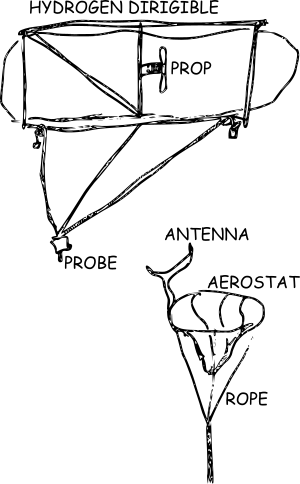
\includegraphics{images/dirigible.png}
\caption{Hydrogen Drone}
\end{figure}

How should motors work for soaring drones? First of all, if the thing is
large enough it can float on the circular current patterns in the upper
atmosphere, holding position with no mechanical work done. But what
about motors for guidance? These motors should be electrostatic, powered
by extremely high voltage giant balloon capacitors which are the main
body of the soaring drone. Using two very light polymers in very thin
sheets with opposite positions on the turboelectric series, it should be
possible when far from the ground to generate \emph{extremely} high
voltages very easily using the mechanical energy source of the rotating
air currents. Electrostatic motors can then run off these, also built
from thin polymer sheets with thin metallization. No magnets and no
copper coils! It's nutty to use the magnetic field for high altitude low
power low speed motors, they should all be based on electric fields,
because it's easy to get megavolts up there.

What about scaling these robots way up in size and weight for use inside
storms? One could imagine giant metal gliders in massive rumbles of 10's
of thousands or maybe even millions of units, all ripping around in a
storm could over the ocean. These generate giant hydrogen-filled blimps
which then gather in a huge rumble to go turn back into useful work near
a settlement or floating factory.

\subsection{Water Robots}\label{water-robots}

Littoral robot rumbles which can use tides and river currents to
generate electricity to propel themselves upstream. They can be
amphibious, use water to charge and land to move, can move with hopping,
jumping, walking, rolling, and slithering. Littoral trash cleanup robots
are fundable, can make a huge difference in cleanup of a waterway, and
also give us free source material for more building.

Another robot rumble I want to build is the slithering water robots.
These use the usual magnet and coil arrangement to create a slithering
motion in buoyant objects, which can then smoothly cut through the
water. The fact that this has not been widely deployed is totally
insane: the same drive can be used in reverse to get electrical power
out of wave action. If the length of each robot is a few wavelengths,
the whole thing will be forced into a wave which can create EMF as the
magnets move, which can go into the storage capacitors, then released to
change slightly the nature of the serpentine motion to direct the drone
in a specific direction.

These can be incredibly powerful technology! The ocean can be a
fantastic source of raw materials for the trash wizards. Note that for
neutrally buoyant drones, this can serve to move them through the water
below the surface. One mode of operation might be to cruise a few meters
above the bottom of the ocean, scanning for stuff to salvage, then dive
and grab rocks to be negatively buoyant once a target is found. With
just barely negative buoyancy, the rumble can float just above the
target as they pick it apart. They then drop the weights, rise up,
inflate bags to float(everything is made from rubber, and reversible
air/vacuum/water pumps are in all things), and pull up and bring
material back to assembly centers, which can also be floating robot
rumble factories. With ocean currents and waves as an energy source, and
no hurry, these robots can work as slow as they have to, slowly making
more and more of themselves until they can have a global impact on ocean
cleanup.

The water based propulsion system also is very appealing for boats. I
want a boat that runs on wave action, wind, and tides, to grab energy as
it finds it, and then use it as needed to move toward a destination. I
can imagine this being just about kayak or canoe sized. I could also
imagine a freighter that is meters or even 10's of meters long. That
sounds small for a freighter, but imagine, again, that they're a huge
rumble that can be easily scaled up. This can be a freight swarm to move
materials across water.

\subsection{How Robots Reproduce}\label{how-robots-reproduce}

Not on their own! With help. Robots can always ask for help, and it is
our task as their designers and creators to build the information into
them in the form of works of art that makes it obvious how to repair and
extend the robot. A robot should also be constructed in such a way that
it is its own means of production: the components of the robot can be
used as a machine to build more robots like it. This will require human
effort, but both the physical tools and the information required to
learn the skills to duplicate the machine are built into the machine and
obvious to find and use. Modern technology is designed to scare you away
from modifying it or interacting with it in any deep way. We seek to
build machines that do the opposite: invite the user to get more deeply
involved, building more, documenting that process, and extending the
technology themselves for others to use.

I will illustrate this with an example. One of the simplest robots will
move itself around looking for energy, then when it finds some(generally
a fast moving water body like a creek) it will turn itself into both a
power plant and a chemical plant, storing energy and chemicals extracted
from the water(targeting human industrial waste of various kinds). This
will involve a computer, some motors and some sensors. Other machines
will be involved in large scale computer fabrication as outlined in
other sections of this work.

\subsection{Cyborgs}\label{cyborgs}

A cyborg, or cybernetic organism, is a combination of artificial devices
and living things. I believe that we should blur these lines both in
ourselves(we have already done that) and in our fellow living things
with whom we should be able to more harmoniously co exist.

One other thing to observe about both ourselves and our fellow living
things is that when examined closely we are almost all in a symbiotic
relationship with other living things. We need our gut bacteria to live,
cows need fungi and bacteria both, trees rely on fungi for their roots
to be robust, which ensures the survival of the whole forrest, etc. The
responsible development of cyborgs should combine living things with non
living things in a thoughtful and artistic and compassionate way.

I propose that the more communication oriented of our fellow living
things should be given access to our communication networks. I have no
idea what happens if you build a virtual reality headset for a octopus
or squid and allow them to communicate with other squids thousands of
miles away. But if they can put their heads in or not on their own,
surely it's worth trying? Perhaps we could allow them to smoothly join
our society, and co exist with us if we allowed them to communicate with
each other using our tools first. A truly symbiotic relationship with
cephalopods might end up with an arrangement where we help them live
good lives using our control of the oceans and our sensor systems for
weather and they use their bioluminescent skin as display technology for
some networked communication devices.

I would note that both for these water based creatures and for the
various flying creatures including insects, birds, and bats, their
brains may allow them to control flying drones with much better skill
than we can, and in large rumbles with much better flocking ability.
Perhaps another virtual reality rig is called for, allowing birds and
bats to connect with huge soaring drones so that they can expand their
minds the way we do with our machines.

\begin{figure}[htbp]
\centering
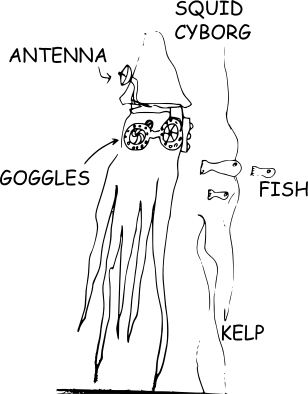
\includegraphics{images/squidcyborg.png}
\caption{Squid Cyborg}
\end{figure}

\begin{figure}[htbp]
\centering
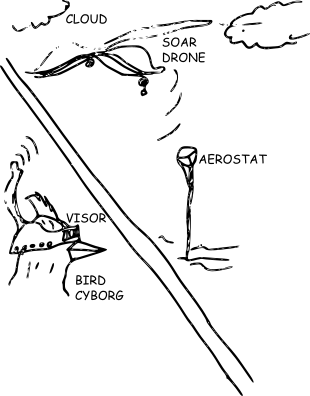
\includegraphics{images/birdcyborg.png}
\caption{Bird Cyborg}
\end{figure}

We should not limit cyborg development to the obvious animals! Plants
and fungi and various strange micro life should be also investigated at
all levels. What would a slime mold cyborg look like? Something awesome,
one might hope. And finally plants, when integrated with technology, can
suddenly move! This leads us to the super ent, which is the next
section.

\subsection{Super Ents}\label{super-ents}

The fractal mater reactor should be alive. Trees, bushes, grass, etc.
can grow all around it, with roots going into various fractal channels
which provide nutrients. These liquid spaces can have various animals
and fungi and microorganisms, creating a whole ecosystem. Imagine an
island built up of such mater, the size of a small building, covered
with trees. Ambient energy is used to slowly build up and discharge
electrical energy to operate philosophy engines which slowly walk the
whole thing across the landscape. With little or even no human
intervention, this limbering living giant might spend decades crawling
up and down hills scouring for junk cars, which it turns into a ever
growing robot rumble that it can give away to any passing humans for
free at any time.

Building this kind of thing in the ocean can be incredibly powerful.
Whole floating islands filled with fractal reactor technology can wander
the high seas, with the humans all underwater in bubbles to ride out
storms, picking up storm energy and sea junk, and building a every
larger floating city deep out in the ocean. This aquatic fractal techno
city could exist even in a dead world of violent storms and acid oceans
and extreme heat.

Machines that comb the ocean for contaminants, using waves go get energy
to move around and sort and grab stuff, potentially floating around for
years before being found based on a data stream that pulses out
periodically, and eventually another type of robot tending robot can
grab it, extract the materials it's gathered, and bring it to a floating
factory robot rumble. This kind of robot is important for the ecosystem
of the jungle city in the ocean-inundated coastal post apocalypse.

\subsection{\ldots{}And a World To Win!}\label{and-a-world-to-win}

The Anthropocene is here. Like it or not, it's here. For the next 1000
years our planet is going to be dominated by the actions we choose to
take as a civilization. If we stay on the track we're on, the atmosphere
and oceans heat up, massive desertification destroys wet ecosystems
while rising oceans eat most of our cities, and the oceans become a
toxic waste dump that cannot sustain life. If we do nothing that is
clearly what will happen. Or something worse involving nuclear
holocaust. Given these alternatives, what difference does it make how
drastically we change things in the sea, air, and land? The opportunity
to simply not let civilization get big enough to destroy the world has
long passed us by now.

So is it so wrong to imagine the whole landscape filled with these
lumbering rumbles of rolling, slithering, hopping, and gliding robots?
Is it wrong to let them reproduce with human help, but with very little
labor-time, allowing groups of people to build endlessly expanding
rumble spheres around the world to create a world of total abundance? I
say that it is not wrong. Maybe if there were a way to go back it would
be a hard choice to do something that disturbs the balance of nature
like this, but there isn't.

This is what the trash wizard wants to make possible in the world:
endless streams of material and data moving through the physical world
with robots made from trash, which encompass our whole human
environment. Maybe not the whole world, but enough of it. A world of
abundance using the rumble sphere and value circles could exist outside
of the states and corporations. It does not need land, just someplace to
move to--it is all mobile by default. The trash wizards build the needed
expertise up and document it and teach it so that any group of people
can create this kind of culture anywhere, specific to their individual
cultural needs and the available resources in whatever geographical area
they're in.

\newpage
\begin{figure}[htbp]
\centering
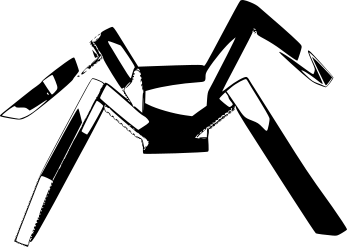
\includegraphics{images/contemplations/contemplation6C.png}
\caption{Sixth Contemplation}
\end{figure}

\subsection{Sixth Contemplation:
Spiderbot}\label{sixth-contemplation-spiderbot}

Go to an overlook, and slowly color in the spiderbot while contemplating
what the land below you would look like covered in free robots all
moving around creating infinite abundance. See the robots! Just sit and
look.


\chapter{Free Drugs, SlimeZistors, and Ion Magic}
\subsection{Technology Should be Slimy and
Dirty}\label{technology-should-be-slimy-and-dirty}

Look around you. We are bags of salty dirty water, and we are surrounded
by mud and dirty rocks on all sides. This is the world we live and grow
and thrive in. It's how our food grows, it's how our waste is disposed
of, it's how we get our raw materials and how we dispose of our
``trash''.

And yet this is not how our technology is.

Our technology is, instead, obsessed with the clean and ``pure''. It is
obsessed with order, with perfect rows of things, with straight lines
and perfectly geometric circles. The very structure of all our
technology represents our worship of numbers and math and military
order, as well as of mining and minerals.

I will go into more detail on this later, but I believe the structure of
the modern micofabricated circuit is a product of the white supremacist
ideology of the far right lunatics who started Silicon Valley. They
were, like all of their kind, obsessed with ``purity'', order, and
forcing everyone to march to a perfectly timed clock. This is borne out
in a machine architecture which they pretend is a product of some kind
of technical evolution but which is just as much a function of their
capitalist religion as the rows of decorative stone columns they out
outside their buildings of power.

If, rather than Evil Machines, we want our technology to be more human
and more life like, it should resemble what we see around us in the
living world. This means it should be largely filled with and immersed
in dirty water. And should be capable of moving fluids and gasses around
at around atmospheric pressure, with simple circulation systems.

Another key distinction of living systems is that they do not
distinguish between material transport, data transport, energy and
electrical transport. All of these involve the flow of ions and various
big molecules through fluids.

Our non-living technical systems crudely split these functions off from
one another.

\subsection{What is Fluidics and why do we
care?}\label{what-is-fluidics-and-why-do-we-care}

One type of magic that must be wielded if we expect to have a decent
life is potion making. This means mixing fluids, moving them around with
pumps, compressing them, running electricity through them, and also
doing things with gasses of various kinds. This is needed to efficiently
compost waste at a high speed safely and to build up plant growth
infrastructure fast for food production. It is also where novel
chemicals and various life saving drugs come from.

\subsection{Light Magnification and
Projection}\label{light-magnification-and-projection}

Build lenses into sticks that can magnify and project the magnified
image. With the ability to project microscopic things, it should be
possible to do real time display with millimeter scale vibration of
fluids and suspended objects in fluids. This could be the free analog
scope I've been looking for.

There should be both a projection system and also a system for direct
projection onto the eyeball of the user in a goggle configuration.
Essentially the standard microscope configuration but with better
ergonomics.

\subsection{clean water}\label{clean-water}

clean water is CRITICAL, need to research existing tech here, talk about
alternatives.

\subsection{Rants about free transistors vs.~Fascist
Transistors}\label{rants-about-free-transistors-vs.fascist-transistors}

\subsection{from the blog:}\label{from-the-blog}

The channels in the reactor should not just be able to take water, water
should be in them most of the time. If the reactor is just barely
partially submerged in water, it can get power from waves and tide or
current in a river or stream, both for generating electricity and as a
direct source of hydrostatic pressure to push materials from one
``side'' of the fractal reactor to ``the other''. I put scare quotes
around side and other here because it's not really going to be arranged
as a simple in/out machine, but will have many channels that direct
materials around.

Having the channels be filled with water means that robots can be made
to be neutrally buoyant or close to it, and propulsion along the
channels of the system can be caused with pumps rather than some kind of
motor on the actual robot. Thus a ``dead'' robot can be directed to a
location in the system without being powered up at all, then can park on
location where the work is to be done and absorb energy from flowing
water to use to do mechanical and/or chemical work on location.

The motion of the water can be used to generate electricity which also
splits water into gaseous hydrogen and oxygen. Pumps could be used to
liquify the H2 in some cases as a more dense energy storage medium.
Having oxygen available all the time is useful for chemical reactor
chambers because you can use oxygen plasma to clean surfaces in an
aggressive way to ready a chamber for a new process. And H2/O2 gas torch
can be used for melting glass and various simple welding and heating
tasks. Finally the re-uniting of the H2 and the O2 will create pure
water which is needed for humans and plants.

Just the wave or stream powered desalinator and burner that can run with
no intervention is a technology very worth building ASAP. Running water
can turn a turbine that makes DC AC power which is rectified and
smoothed to DC, then drives electrolysis, saves it up until a gas
reservoir fills, then an electric spark from a step-up transformer from
the generator fires, reuniting the O2 and H2 to form pure water, which
falls into a water reservoir which can be of arbitrary size. Over time,
this could sit for months building up fresh water very slowly, making it
always available in that location. This must be built! If it's possible
to use the metals in gas powered cars to build fuel cells, this could be
the basis of a primitive hydrogen economy.

In addition to power, locomotion, hydrogen and oxygen, water can provide
many other useful chemicals, many of which are unwanted contaminants
which will be removed from the water over time. Ocean water in
particular can yield vast chemical wealth from the trash found in the
ocean as well as energy from the tides and waves which will be
substantial in many places. Unlike a river, in the ocean one can build
out in a 2 dimensional area and always have both energy and materials
that scales up with the building. Why is this relevant? Because this is
the future of many coastal cities. As our climate shifts and sea levels
rise, many coastal cities will be flooded. Some will be rebuilt higher
up with landfill, with water pumped and managed like in Amsterdam. But
many will inevitably be abandoned. This has the potential to be a
environmental disaster of its own right, as the many toxic chemicals of
a modern city suddenly can flow naturally out of the city.

However it's also a huge opportunity for the trash wizard to build the
means of production. As the refuse of a dead city first starts to float
freely, if fractal reactors and rumbles of robots etc move in fast
enough, the entire mineral wealth of the city can be reclaimed into the
new system. Vast, scalable, production of fresh water will enable a huge
canopy of vegetation to be grown above the site, using the buildings as
a lattice for upward growth to create a green paradise where humans will
move from place to place via skylines of various kinds, some manual and
some powered by electricity or wind or tide, as well as boats of various
kinds. Storms and floods should be able to be captured in terms of both
energy and materials, building up huge amounts of pumped-uphill water as
well as hydrogen and oxygen. In some cases it will make sense to run the
reactor as the storm hits to use very high power levels temporarily to
complete a large industrial task quickly with the surge in available
energy.

I want to make one more point about reactor chambers in the fractal
thermoplastic system. It should be possible to change the shape in situ
using the various assembler robots that can carry heated reshaping tools
around. It's probably easiest to do this in either air or vacuum or some
inert gas, but that can always be done because vacuum and gas pumps are
ubiquitous in the system. I think we also need ball valves that are
driven by the magnetic motors. But if you want to do an edit, you can
always use fluids to move your robots into place, move them into a fixed
position, evacuate the chambers, run flown water through a neighboring
location, generate power off that, create heat and motion and use the
robots to use melt tools to weld, cut and add plastic to make new
shapes, motors and tools.

Three dimensional mater that is made from pure trash and ambient energy
which has the power to edit itself. That is what this technology is
pointing toward and I'm not seeing anything that stops it from
happening. Unlike the Drexler/Merkle model of nanotechnology, this
fractal approach does not start out nano. It will be useful immediately,
and will continue to be useful(indeed revolutionary) even if the
nanotechnology never works.

One more point I want to make is that this technology allows for all
sorts of scalable bio-reactors to be built, so that all the advances of
biotechnology can be leveraged into our free infrastructure. Drugs and
other very useful chemicals can now be synthesized by genetically
brewing with genetically modified organisms in the same way that beer is
brewed. The ability to scalably manipulate liquids should allow for both
the development and deployment of genetically modified organisms to brew
useful chemicals. The ability to make drugs and vital nutritional
supplements in this factory is critical, and again, is a technology that
on its own is worth developing even if the whole rest of this plan
didn't work. Given the fractal nature of our technology and the fact
that it's immersed in water, organisms of all kinds can flow in and out
of it, and be used for many purposes. A symbiotic relationship can and
in fact must be developed between the smart matter technology and the
surrounding ecosystem. Looking just at the flow of atoms, there are lots
of atoms that the human body could use to live in ocean water. Could a
system like this produce a food of some kind just from flowing seawater?
Maybe. With enough energy and time(both of which a patient society has
plenty of) it might be possible to live 100\% off the ocean.

Obviously human and other animal waste must also be processed in this
fractal reactor system. Again this is a source of incredibly useful
atoms. Just the methane that leaks off from solid waste is like gold for
early work on the nano assemblers since it can be used to make 3d carbon
nanotechnology electronics and described above. A living system should
be able to digest waste much faster and more safely than the current
systems where the only living thing is the one target organism that does
the digesting. And of course the reclamation of chemical wealth in the
form of drugs and minerals will also be of huge monetary value in the
old economy quickly, creating a ready source of central bank debt wealth
for the community who lives off the Reactor in the sea cities.

\subsection{another blog post:}\label{another-blog-post}

In reference to the previous post, on the fractal factory, I have been
thinking more about the materials to use. I have been thinking about
silicones for everything. But why? The basic principles in the previous
post will work best with some type of thermoplastic, because that can be
done easily with the free metal etching tool to make moulds. heat,
pressure, and a scanned high voltage welding tool can make layers from
any of these types of material. A scanned heated head could also just
make shapes, and of course there are 3d printing techniques.

Here is a list of some thermoplastics:

https://en.wikipedia.org/wiki/Thermoplastic

PLA, nylon, ABS, PMMA, HDPE, LDPE, and even teflon can all be used!

Also, the correct way to fabricate arbitrary 3d objects from many layers
of thermoplastic is as follows. First, metal parts are made by a
combination of machining, 3d printing, and laser cutting. These could
also be chiseled manually with robotic vibrating parts. High mechanical
impedance vibrating tools with cutting steel and diamond cutting tools
chipping like a beaver's teeth, being moved around with scanned x y and
z motion could cut arbitrary curved surfaces into metal.

All these various metal tools can get picked up by robotic arms and
moved around and pushed into a target material, where the metal tools
are heated to the correct temperature to reform the plastic. This allows
tools to fall over a range of size. The same infrastructure can be used
to deploy a several cm tool to cut a several cm channel in a big block
of plastic, and then micron scale tools also press patterns into other
smaller locations. This scaling of tools means that the fractal nature
of the finished product is represented in the fabrication method.

3 dimensional mechanical thermoplastic lithography. Robots must be built
which can carry out tasks with heated tools in various locations and
scales.

The task to start fabrication becomes clear. To start off, metal parts
are salvaged of various shapes and sizes, heater wire is wrapped around
them with thermometers and temperature regulation, put it on the end of
a stick of some kind, and impressions are made in different
thermoplastic trash from cars and similar household junk.

Going back to the various motor designs, it should be possible to design
the lithography tool set for making the bits out of various
thermoplastics to get all the basic motor types to work. The path to
making all these things work keeps getting clearer. With fluid
transistors that can be fabricated with channels in plastics, simple
logic gates can be made, as well as various types of control and
amplification. With robots that deploy all shapes and sizes of thermal
press tools, it should be possible to make arbitrary 3d fractal channel
structures. This means we have transistors, motors, and pumps. With the
high voltage generator technology working it should be possible to build
it out of the fractal trash foam. Wires can be pulled through channels
by rolling robots of all sizes, and they can go into the liquids to
connect them. Wires separated by a small fluid chamber can make a high
current transistor.

So the elements that are coming together in this vision are: Rumbles of
robots can rip a car apart and make assemblers, motors, processors,
energy storage devices, high voltage generators, high current
generators, pumps, compressors, and finally more robots. Plasma and
chemicals being pumped and mixed in the plumbing allows for arbitrary
synthesis of needed chemicals, machines, tools, and electronics.

Just the fractal robotic fabrication of thermoplastics found in trash is
worth pursuing as an isolated technology. Add that to motors! Chemistry!
CVD! wow! If this works based on even just using piles of trash and
heater wires with sticks used by hand, it can be used as a demo for
getting funding and doing useful fluidics.

\subsection{and another:}\label{and-another}

One of the layers in the trash wizard technology is microfluidic
channels that can move ionized gasses around. The implications of this
should be examined. Ionized gasses are an essential tool in modern micro
fabrication. With plasma plumbing integrated into everything, all the
tools of standard microfab are also integrated. Thus it could be
possible with micro sized plumbing and materials moving vibrational
motors and pumps to fabricate electronic components, move them around,
physically re-assemble them, and break them down and reform them into
other devices.

This can be a path to scalable synthesis of nano devices. Carbon
nanostructures could be built and also positioned by flowing gasses that
are used for CVD synthesis through a channel that then defines the
position of the structure once it's fabricate. Perhaps use of a standard
CVD nanotube recipe where the catalytic particles are positioned using
the particle movement tools described above, and then where more
vibrational motors built into the channel are used to create junctions
of various kinds to create arbitrary nonlinear circuits.

In order for all of this to work, we first need to have a scalable
fabrication system for making micro fluidic channel circuits with pumps
built in that can work for liquids, gasses, and tiny solids. I believe
that a great starting material for this is PDMS. Unlike some other
silicone choices that could be used for the fabrication, PDMS flows with
time, temperature, and pressure. A scanned probe that deforms metal
could be used to get a very high resolution shaped surface. This can
then press a sheet of PDMS up against a flat metal plate, and with
applied heat and some time a perfect copy of the metal should be made in
the PDMS. This could be done to make a sequence of layers, which can
then be stacked and pressed with moderate heat and time to join them
without destroying the shape of each layer too much. Many layers can be
added up to make a 3d network of channels. Some channels will have
conducting fluids in them that can control the potential of various high
voltages. High voltages are used, with feedback, to drive various floppy
and also springy bits of silicone. These flaps, fins, spines, rods,
pushers, and membranes will act to move fluids, solids, and gasses
around the network.

With the ability to move anything to anywhere in the 3d network of
silicone, we can connect the whole cube to various input gasses and
liquids to do chemical synthesis. This can also involve various types of
chemical and physical vapor deposition on solids that are moved around,
connected to high voltages, plasmas, etc. So arbitrary nonlinear
circuits should be able to be built into the superstructure using a
variety of technologies, which grow and shift over time(while keeping
the PDMS matrix unchanged). This is very powerful, and justifies a
potentially laborious and slow build up of the 3d silicone matrix. If
one fabrication run can yield many generations of technology, it can
afford to be slow.

Perhaps the first practical step is to build the high voltage generator
that is part of trash wizardry. If we had high voltage, we could start
playing with electrostatic motors and also would have a source of high
voltage for trying to do scanned probe nano machining of metal surfaces.
The way this generator might work is a mechanical oscillator will be
driven by the standard philosophy engine magnet/coil driver, and will
have appropriate metal and insulating pointy and not pointy bits that
move charge from ground to some isolated electrode. Experiments with
these types of oscillators could begin at any time, and need almost no
funding, just time to work on them. With high voltage working, motors
are needed, as well as welding tips. Then scanned probe weld fabricators
are made which are driven by simple electrostatic motors and can make
molds for PDMS. From here, a system is built up for making arbitrary
networks, then chemical and physical synthesis is built up.

Another important point about this whole technology system is that it
should be fractal scalable. That is to say, there can be channels and
pumps and switches and so on that are as big as meters across in some
massive factory block down to 10's of cm, cm, mm, microns, and finally
down to just a few nanometers. With motors that also scale all the way
up to huge movers of many kg solid objects using coils and magnets down
to electrostatic drivers that move plasmas around at the 10 nm scale to
fabricate new nano materials, it should be possible to take in raw
trash, rip it apart fractally, move destructor robots around as needed
to keep it all apart and sorting it, and at the end the scale is
nanometers both of the input and of the output, which are nanoscale
electronic materials. These materials can be moved around on other
``sides'' from the inputs, scaling back up as needed to create arbitrary
technology with nano structured material.

Can this all be built up from cars? I believe so, as long as some rubber
can be found in cars that can work for the synthesis of the
infrastructure. That probably won't be PDMS, but I believe tire rubber
can be made to work with some experimentation. Fart gas from various
animals and hydrogen and oxygen from electrolysis can make a fair number
of initial processes to start building up technology with. This may be
the future of domestic cattle: as a source of methane to use as a
process gas for fabricating carbon nano electronics. One can imagine a
giant dome tent which channels the methane away from some cows and pumps
it into the nano assembly. Rotting turds can also be used to source
methane, which can be huge piles of accumulated dog poo in urban areas.

I'm suddenly contemplating how the many elements should communicate. I
think high voltages turned on and off could be used to create electric
dipole sources that can transmit at low frequencies and speeds very
easily. For very low data rates, as a constant baseline, all the
elements of the trash wizardry could communicate using high voltage
oscillators controlled by high voltage liquid transistors.

Also note that it should be possible to quickly do science to
investigate new ways of doing things. For instance liquid transistors of
many different liquids should be able to be very rapidly investigated
and instantly deployed after discovery.

It appears that it should be possible to create a totally scalable
nanotechnology system that can break down old cars and create arbitrary
new nano electronic and mechanical materials, which can create still
more factories, made from the same materials which absorb large and
larger numbers of cars, etc, creating exponential consumption of cars
until there are no more cars.

all the stuff about the evils of the microprocessor ideology goes here,
the white supremacy ideology of William Shockley and how that is
reflected in the bad decisions made in developing the modern microchip.
evils of clocks, connection to number worship and monotheism, sparse
desert of the processor, evil separations between matter and information
and energy


\chapter{Magic Tales and Magic Lore}
\subsection{Moving Beyond Money}\label{moving-beyond-money}

Money is a failure. I have gone into some detail about this in the
earlier chapters and I will attempt to not belabor it here. How, exactly
does it fail, though? I say it's wrong to add up human value using
numbers, but what exactly is the mechanism by which this causes so much
misery? There are many mechanisms, but one that I think is worth
starting this chapter off with is its dissipative nature. As money flows
through our society it dissipates. At each stage from the banks out
through all the people working and selling things and paying each other
to when it comes back to the bankers, money is ``lost'' along the way,
usually to various parasitic organisms like landlords and online payment
gateways that add no value but simply take from the system.

So one feature I believe we need to look for in a value system beyond
money is that it should be additive rather than dissipative: rather than
transactions making value decrease, as they do for both money and the
physical goods capitalist claim as ``property'', we want value to
\emph{increase} as transactions happen. This goes against everything
capitalism stands for, as it doesn't work with currency based on integer
numbers, mining or human misery, but that's the point. The fact that
there is ``not enough money'' to do all the many things that need doing
in our society is partly because most of us do not have the ability to
make it. We can get it from someone else, but ultimately they had to get
it from someone who got it from someone who got it from a banker and of
course all those transactions paid the dissipations tax to the various
parasitic rent collectors. We can't just sit down, think really hard,
make a thing, talk to some people and \emph{make} something of value. We
can make a thing then sell it for money, but that is no longer a closed
system. If there are just the two of us, alone in the woods we cannot
create value in the money based system without also involving a banker.
Any system of value that we use to replace money must have the ability
to grow in value and scale in a closed system, without any need to
communicate with bankers, governments or others of their kind.

It is also worth at least mentioning the so-called ``alternatives'' to
money in the form of electronic currency like Bit Coin and the ``time
dollar'' or other currencies based on selling hours of your life away.
These are all still money. They use numbers to represent value, and
address almost none of the underlying problems with modern money.

In the special case of Bit Coin the creators have actually managed to
build perhaps the only money system worse than central bank debt
currency. They have replaced central bankers with members of the
technocratic priesthood who answer to no one and are some of the most
unpleasant and anti social people in our society. And they have replaced
an inflationary system with a deflationary one, making currency ever
more scarce as time goes on. I wish I were creative enough to have
invented Bit Coin as a sort of counter example of technocratic
capitalism gone mad, must like the Schroedinger's cat story used to show
the absurdity of quantum superposition(which still appears to accurately
describe the world). It would have been a great thought experiment to
show in a series of amusing anecdotes just what a horrible idea this is,
but alas, this is not fiction and we all have to deal with Bit Coin
people for the foreseeable future.

\subsection{Infinite and Infinitesimal
Value}\label{infinite-and-infinitesimal-value}

When you say you want to move beyond money for keeping track of value,
the capitalist will typically turn purple and start spitting about how
absurd the very idea is of doing anything like this. They have been
trained to do this, and it's a part of the immune system the capitalist
machine has built up over the centuries. However, they know perfectly
well that values without any numerical equivalent are quite common in
and essential for our society in even its current form. Our society and
indeed all societies have concepts of value outside finite number. Both
``priceless'' and ``worthless'' items are quite common in any system.

That which is called ``worthless'' by capitalists are often the feeds we
will use as ``Trash'' in Trash Magic, infinite supplies of things given
zero numerical value by the capitalists. Returning to the example from a
earlier chapter, the dog turd on the side of a street is an example of
something viewed as ``worthless'' or ``trash'' by the capitalists. To
take this example farther, what would it look like to attempt to apply
capitalist ``economics'' to the dog turd? Over some days it will be
digested by insects, bacteria and fungi. Once some atoms from the turd
have been consumed by a fly, does the fly own them? Who owns the fly? Or
perhaps the fly is a liability, whose is that? If the fly is eaten by a
bat who then uses those calories to also eat the mosquito which was
going to give me malaria surely the fly is now an asset, but whose?
Mine? Or the bat? But who owns the bat? And if I return to the turd a
couple weeks later and it's gone, did it ``depreciate'' to use the
jargon of accountants? Depreciating assets can generally be written off
as a discount on your taxes in most countries. How would I do that for
the dog turd? Perhaps if the turd was on land that I owned and I had a
numerical tally of the molecular wealth in the turd I could then
calculate how fast the flies are taking away this great wealth and
somehow turn this into numbers and then a tax write-off. But surely the
molecular wealth in the bellies of the well-fed flies are now an
appreciating asset. Is that then to be taxed? Who owns the flies? It's
all just nonsense! The vast universe around us of ``worthless'' things
proves the extreme limitation of the capitalist worldview to even
basically describe our environment.

But what about the ``priceless''? This is also an extremely familiar
concept in every capitalist society and is also one in which their
methods of assessing value completely and catastrophically fail. When it
applies to an individual this is usually called ``sentimental value'',
and applies to well-loved personal things. This might be a t-shirt which
was purchased for very little and is too worn to still wear but which
was worn on some long journey. More often themes valuable personal
treasures are those which were given to us by others. We also use the
concept of priceless to refer to those things with shared cultural
value. Perhaps a capitalist can put a numerical price tag on things like
the various stone temples of our different human societies from
centuries past, but we all know that is not the real value. When a
ancient temple valued by the local government at some arbitrary number
of units of bank debt is destroyed no one in the world would dare say
that this is really the same as that much bank debt being destroyed.
It's not the same, because there are values in these cultural artifacts
which cannot \emph{ever} be added up using numbers.

An example of priceless value familiar to some students of American
popular culture is from the film Pulp Fiction from the 1990s. A
character played by the spectacular Christopher Walken presents a watch
to the son of his dead friend, and in one of the greatest monologs
recorded on film explains the priceless nature of the watch in the form
of a story. The story is not about the watch itself but about what
happened to the watch--it's not really about the thing but the people.
The watch ends up representing a four generation story of a male family
tradition of warrior values. Within that culture it has truly infinite
value. All this is shown as a flashback for a main character, to explain
why he is willing to lose everything including his own life to save the
watch. None of that is to tell time, to store value for retirement or to
hoard metal. The value of the watch is \emph{entirely} based on human
values and cannot possibly be translated to finite numbers.

I would propose a system of values based on these ideas, where we all
have our own personal Christopher Walken in the history of the things we
hold dear telling the best possible stories which give things value the
capitalists cannot possibly add up with numbers. There are many ways to
do this. In the end what all of them have in common is that they lead to
a value system that takes more from the study of folklore than from the
study of numbers.

\subsubsection{outline:}\label{outline}

\begin{itemize}
\tightlist
\item
  More on what is wrong with money, briefly, additive vs.~dissipative as
  key issue, need to free money from control, any control, bitcoin
  solves nothing, barter solves nothing, capitalist money diagrams and
  more of that, federal reserve debt, slavery reparations
\item
  value based on not numbers, but on ART, concept of ``priceless'' and
  ``worthless'' and ``trash'' and magic
\item
  oral traditions, tales and lore, folklore as a holder of value
\item
  the feed, a powerful metaphor
\item
  circles and other geometry as symbols of value
\item
  transmission of physical artifacts: couriers and
  thing-streams(skylines, rivers, various wandering drones)
\end{itemize}

\subsection{Magic Tales and Magic
Lore}\label{magic-tales-and-magic-lore}

I'm changing the name of the post capitalist system from ``value
circles'' to something closer to ``magic stories''. ``Value'' is a
problematic word since it sounds too much like an equivalent of the
capitalist economic system. I think it invites too many annoying
capitalism questions, and points the wrong way. And ``circles'' was
maybe a bit of a nonsense word in the way I was using it. What the hell
does that even mean? So I'm dropping both words.

One possibility I've been kicking around is ``narrative'', but that
sounds too impersonal, and too technical. I think ``magic'' sends the
right message since it is so clearly a turnoff word to engineers. One
thing that is clearly emerging here is that engineering as a discipline
and engineers as a culture are my enemy here. They are an important part
of the immune system of the Capitalist Monster that we are all parts of.
It is no accident that engineers like to tear down everything anyone
says all the time, being among the worst ``mansplainer's'' on the
planet. This is because that's where the rubber meets the road for
capitalism protecting its interests. The asshole male engineer who
always tells you you're wrong and nothing will work is really
capitalism's immune system, and in that context their behavior makes
perfect sense.

Possibly ``tale'' is better than stories. ``Magic Tales'' could also
then be abbreviated to ``tales'', which inevitably it would be. After
all, when one says ``tale'' instead of ``story'', does that not tend to
imply Magic? I think it does. Maybe where this should all end up with is
``tale''.

TALE: this is really remarkably easy to understand, and removes the hard
anti engineer bias of ``magic'' with something more flexible. Every
thing has a tale, every person has a tale, they are all woven together.
Perhaps Lore should also be used, and there is a lore data channel and a
tale data channel. Lore is how to build a thing, where to get more,
technological data. Tales are the story this specific thing.

Lore and Tales shall replace economics, and this becomes easy to
understand and explain without getting mired in pointless discussions
about capitalism. Because telling stories and lore has always existed
outside of capitalism, and can co-exist from the beginning. I'm pretty
sure HTML5 is the format, at least for now.

This is part of how Trash Magic can drive wedges into global capitalist
culture: we inhabit the strange corners of the current capitalist regime
where property-based values have not totally extinguished all goodness.
These include in the water, where property law is more flexible, and in
folklore as opposed to capitalist media, where IP has not taken over the
culture and suppressed creativity.

Note: I'm increasingly thinking that both the tale and lore should be
mostly oral. There will be graphical constructions to show how to do
stuff, but I think the combination of oral and graphical might be
superior to the written word for this, because I want the doing of
things to spread, rather than the empty talk. You have to be face to
face to really teach someone this stuff, so why not keep it offline with
exchanged files not on a techfuck server? It won't slow down
transmission of real stuff so why not? It will slow down the spread of
people talking about our ideas but doing nothing, but that's a good
thing. I want 100\% participation: you either walk away or you actively
participate. Reading blogs and even doing instructibles in your basement
in your house is not that. Those ``makers'' are of no use to this
movement except as a source of some materials and instructions in our
early days. Images and oral transmission is something I can actually do.
And this book. Fuck Github.

\subsubsection{Currency Diagrams}\label{currency-diagrams}

This will be pictures not words.

This is now how I see ``the system''. A circle of debt and power links
all people with business and finance to be deployed as needed to support
the military industrial complex. I no longer believe in the words
``money'' or ``government''. These are both fictions. There is only
debt, power, and the military industrial complex. All of this exists to
use fire to turn earth into debt and power and complete the cycle.
Denominating that debt by numbers which have power unto themselves
without the whole cycle is a unspoken State Religion adopted by all
modern states and corporations.

This is what value should look like:

People do labor using industrial ``waste'' of the old system until it's
all cycled through the new system, using ambient energy which comes
originally from the sun, and the living ecosystem that is supported by
and supports that cycle in circles of value. Circles can be formed large
and small, and involve trust between members of the circle which is
initially fixed and which has a finite lifetime. Circles can have any of
many different possible rules and structures, can live for a long time
or very briefly, etc. They might have as part of their interior various
physical artifacts or not, or various mathematical artifacts or not.

Circles may intersect in nodes which can have their own sets of rules.
The level of complexity of the infinitely expanding system of value
circles and nodes and networks has no serious theoretical limit. I
imagine that the amount of data required to denote a value circle is
always going to be small, even with some fairly verbose ASCII formatted
text about background, stories and rules etc. Media might be needed
which could take up a lot more space, but that should all be linked to
from the core value circle object.

\subsubsection{Creation of Value}\label{creation-of-value}

Suppose I have a motor I have built, and you have need for a motor.
Suppose I have built 1000 motors so I can easily spare a couple for your
robot. You need a robot, I can give you a robot, so of course I give you
a robot. Together, we have created value in the world in this
transaction because you having a robot and me having 999 robots is much
more useful than me having 1000 robots and you having zero robots. MUCH
more!

Right now we have two choices: we can just call it a gift, hand you the
robot, and I can feel like a nice guy. Or I can demand some ``money''
for it, after which we say I ``sold'' the robot to you. I put scare
quotes around these words, as I often do, to denote that I'm about to
reject the assumptions of these terms.

When people say ``money'' they mean debt from the Federal reserve bank,
or some other central bank. That debt has value because it is backed by
the military might of the United States, which accepts that debt in its
collection of taxes. But this is fucked. Why should we need debt from
some military backed bank in order to do this clearly positive
transaction? Surely just doing this adds value to society and we should
be able to denote that without federal reserve debt. But there is not
necessarily any motivation for anyone to make that possible.

So what is the alternative? It seems that the most common alternative is
the Marx-influenced concept of the time dollar. A local currency can be
created based on hours of labor which can be exchanged through a
community without any government involvement, taxes, or any banks. But
that is of no help for our robot transaction. My robots were built by
robots and took no labor. When you get the robot, it will do labor so
you don't have to. By carrying out a transaction that saves labor, we're
decreasing the value available in the system according to Marxian labor
theory of value. Anything that makes life easier creates deflation in a
labor based currency, which users of federal reserve debt can attest to
the horror of.

I propose that a usable way to communicate value outside of bank debt
will involve the ability of people carrying out a transaction to simply
create a marker of the value they mutually created. I also propose that
fancy math will not be the basis of this. Especially fancy math backed
by faith in libertarian neck beard fucks(you know what currency I'm
talking about). It will be based on trust. Trust of the people involved
in the transaction, which moves like a bubble through the untrusted mass
of society.

I propose that one way to do this is for a transaction to be a chapter
in a story, and that that story caries the value. So it works like this:
I give you a robot. We write a very short story about this, why we did
it why it was a good idea, why the robot is cool, etc. Short, to the
point, with some details. Now, I can take this story down to the coffee
shop and say ``hey, man, can I have some coffee, I gave someone a robot
today!'' They say ``yeah, you can have coffee here for the next week or
so for a robot, sure. That's the next chapter of the story. They pass
that along to their milk supplier, who adds another chapter and sends it
to the fence post company, who takes the longer story to an affiliate
coop out in the country who is part of our network, who delivers a much
more substantial wood processing robot machine. A real monster. And so
on.

It's not a fully formed system, but I don't think a good system ever
really will be. It's worth a try, better than nothing, better than
federal reserve debt.

\subsubsection{More on Value Circles}\label{more-on-value-circles}

Another element of the value circle currency concepts is myths. Myths,
legends, narratives, call it what you want. One way to create shared
trust between members of a value circle is to have shared culture, or
folklore.

Do people believe these to be actually true? Maybe. Maybe it doesn't
matter. My view is that existing money already has a weird religious
belief built in of the most dangerous possible kind: that which people
don't even acknowledge IS a belief. The entire world view created by the
monetary system where everyone has to exchange central bank debt is not
related to physical, social, or biological reality. It's a artificial
creation which harms most of the people who without having a choice or
even understanding that they made the choice are forced to live their
lives by it.

One way to combat what is essentially a very conservative religion is to
form a belief system outside it, making the transition from the money
belief system to a new one more explicit than just ``losing faith'' in
money which does not force the concept of money to be treated as a
religion.

What would be an example? I think initially they would tend to fall into
two categories: fan fiction and religion. One of the easiest ways to
build a mythology of a value circle is to do something like base things
off of Star Wars or Supernatural or something. It helps when people know
a thing well enough to have a shared reference easily right from the
start. For people who already have some sort of religion, building a
trust network based on that both formally and informally is an obvious
way to get started. Of course other values would be shared by a value
circle, including technically specific elements like ``meters of 24 AWG
copper magnet wire'', but on top of the specific parts, I believe having
something less quantitative and more personal is useful. More on this
later, this ongoing stack of aspects to the Value Circle.

\subsubsection{On Money and Additive
Value}\label{on-money-and-additive-value}

I hate money, and also love it, and that is typical of people in our
civilization. I've thought a lot about all that over the last year of my
total personal disillusionment with capitalism. I'm definitely against
most of how our ``economy'' works, and definitely in favor of something
else, but it's hard to even know where to start with all that. One habit
I've acquired over the last few months of reading and thinking about
anti-capitalism is replacing the word ``money'' in my mind with
``federal reserve debt''. That's literally what it is, and constantly
reminding myself of that helps me to think clearly about the world
around me and what to do about it.

One thing that I hate about money that I want to raise here is that it
is dissipative. When a transaction occurs, one party transfers their
federal reserve debt to another in exchange for some more real good or
service. That transfer has all kinds of losses in it. First of all, in
the money system the most value that can possibly exist after the
transaction is the amount you started with. Until another party is
brought in, in a single transaction, the amount of federal reserve debt
always goes down, just as the amount of entropy always goes up in
chemistry.

Looking at a system like this it's clear that the best way to accumulate
federal reserve debt is to be the dissipation. One way to do this is
literally to take something from the transaction, which is what paypal
and banks and credit cards and the rest of the finance industry do.
Another is to make money off taxes, as the military industrial complex
does. And a third is to be a middle man in the information channel from
seller to buyer, by being in the advertising/marketing industry. And
indeed I argue that these three types of accumulation are the main power
lines in our society: military, finance and marketing. Plenty of power
and wealth accumulators are all three or some combination, but I argue
that most power in our society is based on these three pillars because
they are the optimal means to accumulate federal reserve debt.
Everything else loses to these dissipations and eventually feeds someone
in one of these three pillars more than your little project possibly
ever can accumulate.

It is not so much my goal here to attack the concept of central bank
debt, taxes, etc. as to think about how to get outside this to add and
exchange value without that system. What I argue is that a transaction
should add a note of value to both sides, not just one, and that it
should require no value on a balance sheet before the transaction. This
second part is extremely critical. One of the crippling problems of our
current system is that it prevents anyone from being self sufficient,
ever. If some group wants to exchange goods and services in a closed
economy they need to first get federal reserve debt from the outside in
order to even have units of currency with which to work. Add dissipation
to that, and eventually they'll always be more and more dependent over
time on the outside world, and be forced to participate in global
capitalism. A system that addresses these problems must allow parties to
agree to do a thing, do it, and create from nothing the value that can
be further passed along to the rest of society. Another critical flaw in
the money system is the negative value of work. We assume that in any
work transaction there is a winner and a loser. E.g. at a gym everyone
has to either pay or get paid, it's assumed that the coaches are losing
something and the athletes are gaining, so they are on opposite sides of
a neutral or net-negative(with rent and taxes etc) transaction. But
surely the coaches also gain? Are they not also athletes? And the
athletes are working just as hard, why is their work somehow
``opposite''?

All this is cleared up by the additive currency concept. Here a
transaction creates a value pair, with half taken by each party. Thus
when a personal trainer meets with an athlete, they each walk away with
a unit of value equal to one times the value of that transaction. Let's
now go back to my motor factory supply chain. An urban scavenger rolls
up on their bike with a big bin of copper wire, and we each record that
that was of value and changed hands. They then take that value token to
the local coffee shop who pours them coffee and both sides get the
coffee transaction token. The coffee shop buys a coffee grinding machine
using one of our motors from one of our customer factories, more tokens
are generated on both sides. The coffee shop takes this new hoard of
tokens and pays their workers, and this payment also generates value on
both sides, further accumulating the wealth of the coffee shop who is a
major pillar in all this. The grinder factory trades with us for motors
in bulk, and some bulk material transaction value is again created on
both sides of the sheet.

There is a strong analogy between this system and the so-called h-index
used in academia. The h index is designed to create a measure of the
success of an academic career based on the combination of two factors:
how many times has someone published and how much are those publications
cited. The idea is to avoid valuing either the one paper that gets 1000
citations or the author who publishes 100 papers a year none of which
are ever read. Authors who both publish often and get frequently cited
are, on average, going to be the biggest contributors to value in the
field. For better or worse, h-index ends up having real value that can
get turned into federal reserve debt by having an impact on hiring and
promotions of academics. It's not a perfect system by any means and is
widely abused by departments but I think it's an interesting proof of
principle that this idea can be useful.

A missing part of all this is a proposed implementation strategy. How
should the value be accounted for? I could think of a lot of ways to do
it but I want to make the point that I think this is much less important
and difficult than a lot of techno nerds want you to believe. Any store
of value, whether it's paypal, cash, or credit card debt is basically
based on trust. Sure, there are anti-counterfeiting measures on bills
and encryption on online transactions. But for the most part these
systems work because most people can be trusted most of the time. If
everyone really were out to steal and cheat, encryption would be nowhere
near enough to save it, and it would collapse instantly. All this works
because the VAST majority of people would rather do something useful
than go into the illegal bill printing business or credit card theft.
One way I think it could be done is with an archive of stories. Some
kind of shared electronic narrative that includes all the transactions
in the network. This is not great for doing illegal shit or avoiding
government surveillance, and that is a problem in some ways. But not in
the long run because it forces people to push back against the
government controls a lot harder and faster and also because that stuff
can always still happen with federal reserve debt, alternate and more
anonymous systems, etc. Clearly there will be others for whom this
doesn't work. But I believe that a story- database-based system of value
can work for some people. And if it works for anyone it's instantly
extremely powerful because it will grow exponentially and naturally find
the people who can benefit from it most. Is it taxable? Probably not. If
we do things ``for free'' meaning no federal reserve debt is exchanged
at all, what is there to tax? Surely not vast, unencrypted databases of
anecdotes and poems describing the actions of millions of people.

And it's not even really necessarily a threat to the government tax
system, I think. Part of how our system is as broken as it is is how
differently it serves those who control the pillars of power from the
rest of us. The fact is that the capitalist overlords, governments,
military machines etc. don't really need the vast majority of us to
exist. Our demands for food, medical care, housing etc. are mostly an
inconvenience to them. An economy like this might take what looks like
potential tax revenue out of the system, but it also takes an incredibly
vast load of social welfare spending off of the existing system, since
that kind of value is so much better created in the additive value
system. One more point is that I don't consider bitcoin to be in any way
relevant to fixing the money system. With any form of currency, you have
to ask ``who do I trust when I place trust in this?'' I have lots of
criticisms of the central banks, and the federal reserve in particular.
But given the choice between central bankers and some neck beard fedora
software montherfuckers, I'll take the central bankers any day of the
week. Because the demographic in charge of bitcoin is, in my view, the
single least trustworthy group that exists in our society. Also,
building deflation into a currency is so bizarrely pathological it's not
even worth looking at. Bitcoin isn't money, neck beards are not
revolutionaries, it's time to move on.

So where do we start? I think I want to build a supply chain out of
trash, and then just try the database of stories method and see what
happens. Having a supply chain that is clearly of value will give me the
leverage to start a thing like this. So probably another year or two are
required, and hopefully by then I'll be more comfortable with python and
will be able to build a prototype software system to start this off.

\subsubsection{Free Feed of the Value
Circles}\label{free-feed-of-the-value-circles}

People love their feeds. Facebook, Twitter, Yammer, news feeds, tumblr
feeds, text message feeds, push notification feeds. It has proven to be
a very widely liked format for a person to see the passage of time of a
community of people. Value circles should include this feed concept.
Working on your stuff will add media content from your device which gets
added to the main value circle database and then fed into various users'
feeds based on their filter choices. I think if you are not trying to
make money that this whole thing can be much simpler than the existing
software and that Facebook etc can be replaced. However, it's also
possible that the best first implementation of this will be to do it in
a existing commercial system like Facebook. This is obviously dangerous.
Dealing with companies like that can have legal problems, control
problems, and limitations on what you can do practically. It's not
ideal, but it's something to consider. And the free feed that circulates
and shares data to a web browser that can be loaded on the pi zero
tablets of the trash wizards is a project that should be worked on
immediately. Probably tools already exist that can be adapted for this
task. This is worth some detail in the first book, it's not physics,
it's code and that's faster to deploy.

\subsubsection{Courier system}\label{courier-system}

I need a courier system to facilitate movement of goods as well as
skills without shipping costs

\subsubsection{Also value trees}\label{also-value-trees}

Is the circle the best geometrical metaphor? Sometimes. But I should
generalize the concept of geometric metaphors to include the spiral, the
pentagram, the tree, the fractal, the sphere, the torus etc. etc. trees
have roots and leaves and branches and a trunk and sap and sun and soil
and water.

\subsubsection{Trash Wizard Interaction with Capitalist
Economics}\label{trash-wizard-interaction-with-capitalist-economics}

We all have to live somehow, and most of us can't just sink beneath the
waves and escape capitalism overnight. We need money to pay rent to live
in a city where our loved ones are, to pay for medicine, get around on
capitalist transit etc. How do we do this ethically without just selling
out?

Here are the rules for Trash Wizard capitalist interactions:

\begin{enumerate}
\def\labelenumi{\arabic{enumi}.}
\tightlist
\item
  Try not to buy raw materials and other peoples labor, salvage trash
  and rely on mutual aid for free, and build your own stuff
\item
  To make money, selling labor is best, then selling stuff made from
  trash, always try to avoid labor and materials arbitrage: don't buy
  stuff then sell it don't pay people then re-sell their labor.\\
\item
  Do not sell misery, try to only work on things that are fun, while
  they stay fun, each product or service should be an ADVENTURE.
\end{enumerate}

We create. As long as our fed debt money comes from our labor and trash,
we will always have a net gain of capitalist currency into our system,
making hte sign of the dderviavie right. sell one off art pieces for
high prices. All my pieces should be unique.

\subsubsection{Specifically The Post Capitalist Sex
Industry}\label{specifically-the-post-capitalist-sex-industry}

Let's imagine a sex industry, with the word industry used, and inside
the capitalist system but without actual capitalism. What do I mean by
that? I mean that people who work make money but that they neither work
for a capitalist nor function in that role themselves. By ``capitalist''
I mean someone who pays one price for something and then sells it at
another price, whether that is wage labor or materials or outsourced
services. Usually they use some economy of scale to allow themselves a
monopoly enforced by the usual forces of armed capital. Exchanging
things of value for currency is not capitalism in that sense, as long as
you don't have to spend money for it.

I will now sketch out a ``business model'' for an anti capitalist sex
industry collective using Trash Magic.

First of all, how do you want work in this system to work? Really what
you want is to get paid about \$2000 for each sex event, to do it with a
bunch of your hot porn star friends who are into cool stuff and live in
your cool neighborhood, and to make art together and also build
something that useful, combining art and beauty.

So let's say that the goal here is to have about 6 people get together
for a queer techno art orgy and each make about 2 grand. That means you
need to make a total of about 12 grand. And you want to build a set of
artifacts which you sell for about 50 to 100 bucks, which a lot of
people will shell out for if they dig what you're doing. That means you
need to make, sell, and ship about 300 units.

So this orgy has to have the right set of robots and other machines so
that 6 people can make 300 units of an art-tech artifact in some
reasonable time. Suppose this whole thing takes a relaxed afternoon to
do, with all your stuff already set up in your Trash Magic Coven Space.
if we divide the number of units by the number of people it's 50 units
per person for the whole event. If each person has about 2 hours of full
participation in them before they get bored or tired, that's about 25
units per person per hour, or one unit every couple minutes for each
person. That's pretty efficient! Very doable with automation, but really
quite efficient and will require serious process optimization, which the
orgy process can help make happen.

Ok, so suppose that after your leisurely drugs/industrial
metal/manufacturing/art orgy you have made, and I'm going to boost the
numbers here, 500 units. You put those in an inventory file, which you
only give to people you put on a vetted customer list. Each unit
contains physical media with video and other data of the orgy for
pornographic purposes, and is a fully functional Trash Magic Stick. The
inventory system starts from scratch with each orgy, where each customer
has a one time customer ID number randomly generated and never used
again. Customer and performer alike then line up times and places in the
database to meet usually in public places, generally with several
customers for one performer and place, with performers always traveling
in pairs for safety to exchange the physical ``art piece'' for 50-100
dollars cash. Thus each transaction is simply money for art, in small
cash amounts(generally exempt from sales tax). All transactions will be
local, and performers will courier the inventory by bike around town.
The number of customers is about 300-500 so for 6 performers each one
can plan on about 3 distribution events each with about 20 customers. So
it's a second afternoon, on top of the first, and with a good number of
people for the events, easily each person could make 2-5k for a couple
days of work. If you did that about every two weeks, you could make
50-100k/year, enough to live a comfortable life where you spend 80\% of
your days doing other free art and science and the remaining 20\% having
orgies with your hot art/tech friends.

Many of us will end up doing serious R\&D during that other 80\% of the
time, enabling our factory to make more and more advanced stuff. After a
few years of R\&D I could imagine the customer getting a portable
medical imaging machine and some synthetic insulin with legit quality
control for their 50 bucks cash.

But what about the current clients, the horny old men with tons of cash,
the sexually disappointed owners of capital? They have to pony up much
more than cash if they expect to get what they want. They want some kind
of elaborate pro domme fantasy? Ok, sure, but they're not going to hand
over a stack of federal reserve notes, they're going to give you 80
tonnes of shipping space on their next freighter out of hong kong and 10
tons of rare earth magnets for your motor production. If they want to
use their position as controllers of the means of production to get sex
from younger, more attractive, and less broken people, that's all fine
but they're going to actually hand over those means of production not
some bank debt funny money.

Examples of what clients might hand over would be vast quantities of raw
metal, permission to work on private land without rent, and a lot of
long haul transport. Given that some captains of industry actually know
something about industry, this might even not be that bad for
performers, especially if people were well matched up in interests.

Also note that all this will be art. As fast as we'll be moving on the
assembly line to both have sex and guide the rumbles of robots, we'll
all also be working on the artistic process of shaping how the products
actually look, as well as putting on a performance that will be in the
final media.

In the beginning, obviously my fantasies of MRI machines and nano drugs
is not realistic, so what will we actually make first? The Trash Magic
Stick will be the first product. This is a simple artifact about the
size of a large walking stick, which can do many tasks that require an
electric motor. It can be modified by the user to have a powerful sex
toy, a mobile robot, a simple manipulator for 3d fabrication, a water
pump, a evaporative cooling unit, and several other useful machines. It
runs off of ambient energy as detailed in my book, usually flowing water
on site.

Yes, that's another thing, the physical site location. Ideally orgies
will take place in an amphibious environment of floating trash boats in
really nice weather, so that there is water power readily available both
to generate electric current for electronics and to do work and to
source water and other chemicals into the various industrial products.
So the Spring Orgy will be huge in this system. From the thaw of the
creeks through summer might just be one continuous orgy, followed by
just swimming and writing all summer and sleeping all fall. Again, if we
have the machines and robots we need, this is possible RIGHT NOW, under
capitalism, living in a nice fancy apartment in a big city and drinking
expensive coffee.

Oh, and how do we do that without getting the government coming after us
for tax evasion? By paying our taxes. Part of the infrastructure that
should exist here is a automatic LLC formation and dissolution as needed
for series of orgy/fabrication events. A company bank account will be
formed, money moved into it, taken out for taxes and distributed as
dividends to all the equal co-owners, then dissolved. So we'll actually
all be paying a very high tax rate. But who cares? We won't be putting
any money in, hiring anyone or working for anyone.

And this can also be scaled up quite a bit as high end pro doms fully
deploy their network of clients to start getting their hands on larger
quantities of raw metal and other critical process materials. We want to
avoid any materials getting mined on our behalf, because that will make
this technology non-free. However, if material is diverted \emph{out} of
the capitalist system in exchange for pro dom and other sex services
that is a net positive.

Lastly I want to consider a use case of this model that's scaled up a
bit, to say 100 people. This is something that could be done on a trash
flotilla surrounded by yachts in the waters outside LA during a sex
industry convention. 100 people come together and make, now with
considerable economies of scale and sophistication, 500 units each over
a week of work, with insane epic orgies of every possible variety. So
that's 50,000 units. And at this point each thing is really powerful,
can do significant high tech shit the capitalists can't do, like
universal medical imaging. So the performers sell them for 100 dollars
each, easily, making a total of 5 million dollars revenue for the
project(and gross = net because we spend zero money). If you divide 5
million dollars by 100 people, you get \$50,000 per person, enough to
live a decent life on for the whole year without any other work, even
after paying a high tax rate(which we should not have to do since this
will be capital gains if we have a decent accountant).

Does that sounds like unreasonably high production rates? I don't think
so. Current manufacturing technology already has huge economies of
scale. If those same scale economies are used with the same physical
basis of our technology but where everything is made from trash during
orgies, and we keep the value, this is really a pretty modest production
rate. With that many people involved, we'll have access to a ton of raw
materials, land, computer infrastructure, machines of various kinds etc.
And is the number of 50,000 customers for this scenario realistic? I
think it is. With mass communication via twitter and the like, it should
be possible to very easily and with no money spent to have the more
marketing oriented performers connect up with that many people in a
large metro area like LA or NYC, and then for each performer to
personally distribute 500 units in sets of 50 10 times by bike around
town. Serious work, but doable, and in just a few days if all the
infrastructure is in place.

With larger economies of scale and more high tech products, it will be
possible to have the products sell for quite a bit more, as well.
Something very high tech that costs many 10's of thousands of dollars(I
really want to build a fucking MRI machine,really want to) might be
built this way, making it still easy to sell the thing for 500 dollars
in this model, making the take home for each performer more like
\$250,000, meaning they only have to do an epic sex manufacturing art
science orgy like every few years if they want.

So this is how I propose the sex industry should work within capitalism.
It is a system where all performers are paid the same, make
\$50-250k/year for working a few weeks a year maximum, only ever have
sex with their hot porn star friends, and don't have to worry about cops
or the IRS because no laws are being broken and taxes are being paid.
Legally, all performers are professional artists, part of a series of
art-selling LLCs selling their own work built from trash.

How the fuck do we actually do this, you ask? That's my job: to build
the robots and write the instructions so that you can do it just by
watching some tutorial videos and downloading a bunch of free
instruction files. Give me another couple years and I think I can get
this working, but I think for very small numbers of units and people I
can get something working by fall of this year: making sex toys I mostly
already know how to make, which just need a bit of work. Art, though,
all art. Oh, yeah and free MRIs and the most powerful vibrators ever
built, running on off-grid power. Boom!

Also note that all this is Trash Magic. So these are magic witch orgies,
using all sorts of Trash Witchery, with associated Magic rituals
involving the process of assimilating trash into the world of magic.


\chapter{The Great Junk Car Feed}
To the beat of the drum:

\emph{ROBOTS that turn junk cars into robots}

\emph{that turn junk cars into ROBOTS}

\emph{that turn junk cars into ROBOTS}

\emph{that turn junk cars into ROBOTS}

\emph{that turn junk cars into ROBOTS}

\emph{that turn junk cars into ROBOTS}

Cars are the enemy of humanity. Every year in the US cars kill over
40,000 people, and maim countless more, similar to the \emph{total}
carnage of the entire Vietnam war which lasted many years. Globally, the
death toll is well over 1 million, or 10 million in a decade. 10 million
dead.

And that is just the beginning. Cars are central to the industrial
system which has crushed our humanity. A huge amount of our oil based
economy is used by the car system, adding to climate change massively,
as well as bad urban air which kills millions worldwide. Cars create a
society in which anyone who cannot drive is disenfranchised, punishing
anyone without perfect health and significant funds as well as the
willingness to actively destroy the world and possibly kill living
things just to get through their day. Cars have filled up the USA with
enough pavement to provide solar power to the entire nation(no small
feat given our absurd energy consumption now). Runoff of oil and other
toxic chemicals leaks from cars into every water system in the world,
poisoning every possible ecosystem.

The companies that produce cars are some of the most evil on the planet.
Several of the major global brands, including all the German ones, have
actively participated in genocide, an act for which they have never been
properly brought to justice. The endless stream of minerals required to
feed the input end of the planned obsolescence conveyor belt also
destroys the world in the ways that mining always does, with its usual
disproportional impact on indigenous people around the world and on many
other marginalized populations.

In America and many other countries, car companies actively work to
undermine democracy and civil society, campaigning to make sure society
is built around the profits of their companies rather than basic
principles of free movement of people. The ability to move from one
place to another within a city for free should be a basic part of any
social contract that people would actually consent to. Car companies
have built a society where there is no universal social contract in
regards to mobility: all mobility is held hostage, under threat of
violence, by a group of psychopaths(all car makers) who force all
transport to make them money. Even ``public'' transit is always based on
giant machines made by the same monsters, and is deliberately priced
high enough to make sure the poor pay at least as much per mile for
getting around as those who have the money to buy into the car system.
Every time there is an economic downturn, the corporate backed local
government will use that as an excuse to further crush the lives of the
poor, raising fares and cutting services at the very time those without
resources are likely to be the most desperate. Again, this shows the
fact that there simply is no social contract in the modern industrial
city which all citizens consented to. There is only the raw law of
force: whoever has the most control of the industrial machines has the
power of life and death over everyone else. Of course the rulers dress
this up in nice language about the ``rule of law'', but there simply is
no such thing. It's a costume raw force wears in our world.

So the car companies and their collaborators in government are enemies,
and cars form an almost living enemy of humanity world wide. What should
we do about this? The Trash Magic answer is always the same: first find
the trash stream(which always exists under capitalism since destruction
is inherent in their ways) and then find ways to organically incorporate
this into something good rather than bad.

And what treasure there is in cars! Name any precious metal or special
type of polymer or gas fitting or mechanical device and you can find
them in a car. A single unit of the modern automobile also has numerous
computers of all kinds, which can be stripped and used for integration
in our electronic systems. And given the spectacular waste of the
current system, cars really are free: while there is a used market for
junk cars, it's clear that for society as a whole the global stream of
junk cars, like other industrial waste streams, is a net liability not
asset. This negative value creates a global and ongoing opportunity for
us to get the parts we need from it.

Another advantage of using car parts for industry is the way in which
the car standardized. There exist millions of units all over the world
of certain popular car and truck models, and it can be possible to very
accurately duplicate a complex design which uses parts from a certain
make and model because of this.

summarize the global car industry in terms of different countries'
companies, corruption involved in car companies, US auto bailouts,
Korean chaebol system, other corruption--this is a purely evil industry.
Henry Ford's naziism and violent anti labor actions.

also global statistics on pollution and killing and mining and land
destruction for paving and killing of wildlife and destruction of
habitat and destruction of our cities and culture and everything from
car industry

present energy consumption, oil consumption, growth of the system

robot infrastructure to rip cars into robot parts

ancient car remains and crushed cars

end game: end all cars

destroy every single car. rip out the individual atoms. Rip them apart.
Smash the engines, destroy any vestige to show that they ever existed.
Rip up the roads. Build structures to live and work and grow crops in.
Make them all green, smash them but don't replace them with private
property, this is a wedge to build more non private property space.

\subsection{all cars must be
destroyed}\label{all-cars-must-be-destroyed}

\subsection{Cars are CENTRAL to our
enemies}\label{cars-are-central-to-our-enemies}

\subsection{As long as capitalism exists, cars will provide infinite
free resources to
us}\label{as-long-as-capitalism-exists-cars-will-provide-infinite-free-resources-to-us}

SO many minerals! Go over the whole list. Destroy a car in Nikiski,
document it.

In the water. Find cars in the water, process them in the water.


\chapter{Factories Everywhere and Nowhere}
\subsection{Slipping Between the
Cracks}\label{slipping-between-the-cracks}

Where can we build? Where can we work and play and live? Between the
cracks. Between the cracks of the industrial system, between the cracks
of empire, between the cracks of cement and steel. Just as we seek to
build from the discarded materials and energy of the old world, we seek
to thrive and grow in the spaces they have cast aside.

As with materials, those spaces are incredibly rich in every possible
way, when looked at outside the value system of capitalism. Often these
spaces are considered off limits by the powers that be, and are
supposedly private property. However the spaces I'm thinking of are not
monitored and indeed must be ignored for the system to work.

The foul waste filled waterways of suburban New Jersey are one example.
Often spaces under freeway bridges are ignored and abandoned yet
centrally located in a city. Abandoned factories are a fantastic place
to re-start industry in the places abandoned and destroyed by organized
capital. The dark, unkempt corners of various parks have places where
someone can vanish from sight and be centrally located with access to
people and infrastructure.

In general, our first choice for location will be somewhere that has
running water. This could be either a flow of fresh water or a tidal
flow, but it is important both for a source of unlimited energy and for
a source of materials. Deep water is useful for being able to move very
large freight such as salvaged trucks or airplanes found underwater into
position to work on in the production zone.

Water also serves as a source of coolness for protection against hot
climates. Evaporation can be used for added cooling power using water
driven pumps. plumbing which can be taken apart, moved, and put back
together should purify and move the water around, making hot bath water
and god drinking water, as well as building the input for the biological
and chemical reactors which will process human waste.

After water and energy, concealment is probably the next priority for
the ``between the cracks'' model. The easiest way to do this is to be
very low key and work on existing land. If you can camp somewhere, and
the Trash Magic industrial production is quiet and small enough, perhaps
you can simply do it un-noticed wherever you happen to be. Setting up in
the factories the industrial system has abandoned en masse in places
like the industrial Midwest of the USA is another great concealment
strategy.

Camouflage in design is also an important tool. We should be prepared to
build infrastructure that does not look like infrastructure. One of the
ways in which the symbology of Trash Magic can be used is in an
extension of Hobo symbology which allows for cryptic marks to indicate
what infrastructure exists where. Part of the art we study is building
working technology which looks like the environment because it simply
\emph{is} the environment: boulders, logs, sticks, rocks, patches of
seaweed, etc. Substantial infrastructure for industrial production of
all kind can be designed, built, and deployed in this manner where only
the initiates in our Magic will even know it's there.

\subsection{Bring the Means of Production to the
Action}\label{bring-the-means-of-production-to-the-action}

Most communists and anarchists direct us to turn the factory into a
place of political action. I propose to do the opposite: to bring the
means of production to the action. Where there are protests or
occupations or refugee camps or war or poverty, Trash Magic can shine a
light in the darkness.

practical considerations, examples, actually go do it and record it and
put it on youtube

\subsection{Production in Autonomous
zones}\label{production-in-autonomous-zones}

One of our goals is to erase arbitrary lines between things that are
currently separated. Just as some people have tried to erase lines
between protest, occupation and party. I want to erase lines between
industry and art, between protests and factories and workshops and
squats. Anywhere there are people and materials there can be industry.

It's worth mentioning that I don't mean just crafts or hobbies or art in
the current definitions. Part of what separates industry from those
activities today is how they all scale. Art gets its value partly from a
deliberate non-scalability. Crafts are almost deliberately set up to be
non scalable as well, to create some kind of perverse joy in doing
things slowly and with a lot of specialized skills. One speaks of a
``craftsperson'' as someone who has mastered some difficult special
skill, and who therefore has special privileges associated with that
skill.

In Marx's day there was such a thing as an industrial worker, and maybe
in some places there still is. The industrial worker is part of a larger
whole which uses economies of scale to change how people, energy and
materials move in such a way that it will always beat out other forms of
production on efficiently and ``price''. This has led to a historical
dead end as the capitalists have carved up the global working class so
effectively. And good riddance! Do we really all want to work in some
giant factory doing identical boring tasks for many hours, even if the
IWW ``owns'' the factory and we all have free food and health care? Fuck
that future. We bring the factory to the streets where the party is,
inject art and culture in it, and make it able to thrive and grow fast
in the current world.

Here's how it happens. Anywhere there are people, energy and materials,
we just start building industrially and creating art as part of that
process. We build processes and document them(this used to be called
culture) which can be spread and expanded quickly, which allow any group
of people with minimal skills to rapidly build an effectively infinite
inventory of useful industrial products such as air conditioners, water
purifiers, massagers, grinding tools, communications infrastructure,
blenders, coffee machines, electric wheelchairs, soaring surveillance
drones, and medicine. All these goods are immediately entered into the
global decentralized database of free artifacts, which allows them to be
immediately taken by courier by hand to users who absorb it instantly
into society.

This totally changes the balance of power in any occupation. If instead
of occupying the center of town and putting ourselves in conflict with
current society we imagine a bunch of yuppies having to go down into a
Sacrifice Zone to get some awesome artifact they can't get anywhere
else, which they also can't pay fed debt for. There is no transfer of
fed debt or ``ownership'', so all the normal regulations that apply to
commerce do not apply. We slip between the cracks to build up the
factory, make stuff, absorb trash, improve the environment by putting in
infrastructure easter eggs, and disappear. Often the people who come
together to do this will simply not exist as a coherent organization
before or after the industrial/art event.

The powers that be know how to protect ``property'' and to keep the have
nots from getting it from the haves. Much of this has to do with
regulating money. What they do not have experience with is free people
giving away free stuff from trash and ambient energy in on and around
their system. They're prepared for a broken shop window, but not a free
beer fountain in the park. They're prepared for a black bloc in the
middle of the town square but not a boat factory in the middle of a
polluted-to-death river. They are prepared for half a dozen commercial
surveillance drone sent to spy on the cops. They are not prepared for
10,000 soaring drones built from trash, soaring over the dead land of
the American West looking for pollution and mapping it for future use by
our industry.

And this process is within reach now!!! I still think the first
industrial process is the coil winding process which is used to make
more of itself. This means both a coil winding machine and the power
tools needed to quickly break down electrical appliances to get the
copper wire out and the infrastructure required to track down rare earth
magnets, as well as power tools to make lots of Skeletron and plastic
parts quickly. So this means drills and grinders and saws and also heat
tools for working plastic, grinding tools for taking stuff apart, and
good sensors for tracking down magnets. Also free decentralized access
to all the needed data. Energy must be ambient, not oil or human.

This set of tactics then informs the overall strategy and vice versa. It
tells you where to occupy and for how long and with whom, at least to
some extent. We need ambient energy. That means the sun, the wind, and
moving water. Moving water is usually going to be the best choice
because the energy density can be so high. With 1000 times the density
of air, a relatively slow river can be much better than even pretty fast
wind. And way more pleasant to work around. Also waves and tides can be
used, as well as in some cases water that has been pumped uphill over a
long time before the establishment of a industrial occupation.

We reflect the industrial occupation of today through the looking glass:
rather than not building stuff in a factory we build stuff in a
not-factory.

So the first choice for a site is on flowing water, with tides and waves
especially helpful. Also note that natural water, even very polluted
water, is also a source of many useful industrial feedstock. At minimum
you have H2 and O2, but usually a vast wealth of other chemicals. So a
very polluted wetland in the mouth of a river is an ideal site. With a
combination of skeletron and plastic we can build an amphibious set of
shelters and transports and food and water production which add up to
self sufficiency.

Then we need materials, raw materials with a clear path to an
industrially produced artifact or set of artifacts and raw materials to
be moved by courier to another post capitalist industry node.

metal and plastic. And wood. And stones. This can be many places. Rivers
with trash in them, with littoral robots that go out and find it is easy
pickings. Also any dump of car or electronics related junk by a river or
lake or sea. And there are so many of these! Sacrifice Zones are often
near water. And usually have unlimited trash available.

We roll in, we build and distribute, set up infrastructure easter eggs,
and move on. While where there, we create a one-off unique culture for
that time and place, which propagates through the physical artifacts
which carry data that includes the artistic culture of that unique time
and place. This also means that the phenomenon that replaces the current
protest model can be more long lasting. Imagine if any of the famous
protests or occupations, such as for instance the AIM occupation of
Alcatraz had been run this way. You could, today, use an artifact with a
piece of iron from a rebar salvaged from Alcatraz and painted by one of
the occupiers there. Such an artifact could then have been used for an
electromagnet in a big motor that ground coffee beans in Zuccotti park
during Occupy Wall Street, which was then incorporated into a sort of
Jawa art car that roams the toxic waste deserts of Arizona, collecting
minerals for another future project, all with added stories and media
and art.

How different this would be! We could all be participating in various
insurrections, art communes, famous science experiments, and huge
parties at the same time, endlessly remixing artifacts that carry all
that culture with them.

I need to find the Sacrifice Zones that exist in the coastal waters of
the East coast.

Searching my memories of such places in Souther Connecticut and also
looking at maps and charts of coastal DE and MD, I'm reminded that
simply finding the ``free'' material input in such a place is non
trivial. What i think I propose instead is the same courier system used
to distribute artifacts is used to acquire raw materials from the trash
of mainstream society.

Also, if production happens in such coast waterways but materials come
from elsewhere it should be possible to disappear. A combination of
counter-surveillance to always monitor the monitors and camouflage and
totally mobile amphibious infrastructure should make it possible to
avoid detection in un-used land indefinitely. This should be possible
all over the world, anywhere there is a fractal water system. The areas
around Boston, NYC, DC, the SF Bay Area and Seattle are all like this,
as well as many of the great cities around the world.

Trash Pirates. Southeast Asia has marine sacrifice zones where ghost
ships with slave crews fish for the grocery stores of the rich world. If
a guerrilla industrial movement were to appear in this environment with
vastly superior technology to the capitalists, we'll see very rapid
change with no physical opposition from the nation-states. Why? Because
they have built a system where they have a vested interest in these
lawless zones existing. They have to either impose the rule of law on
these places and lose their slave-caught industrial fish slaughter or
they have to accept that our pirates can operate outside their ``laws''
just as readily as our capitalist enemies.

What if Somali pirates could offer legitimately better employment than
the European companies the crews of the hijacked boats work for? it's
hard to negotiate for ``hostages'' who don't want to return, and
dangerous to negotiate for them if when they return they all just quit
and disappear into some swamp. Let's fill in all the spaces the
capitalists have chosen to neglect with new industries that combine art
and culture and science and technology as one thing!

\subsection{Life in the Delta}\label{life-in-the-delta}

The future of humanity is in the deltas. just as the past. And it's
easy. SO many cities have out of the way places an amphibious trash
magic industrial culture can flourish without detection. Freight
transport powered by tidal energy driving electrochemical cells can be
used as a universal industrial supply chain, with vast amounts of trash
gathered for free from underwater salvage and swamp and wetland salvage.
Distribution of goods into the capitalist economy in the heart of a city
via water front parks can then easily happen, also under the radar. By
under the radar, I literally mean under the actual radar, with boats of
such a low profile that they are not distinguishable from wave action by
radar. Fabrication will be right on the edge of water and air, with
object able to be moved in and out, water to be sprayed and pumped and
mixed.

The capitalists have had nanotechnology all wrong. They have been
looking for a clean technology with perfect control. That's wrong. You
want only fractal control, and very dirty, to in fact eliminate the
concept of dirty. Dirty is a capitalist delusion. Must look beyond it.
Under water, fire is also less of a hazard. H2 and O2 plumbing
everywhere, as well as compressed air, fresh water, DC power, various
materials which can be sent in tubes via plastic cells that get pushed
along and tracked. Just the ability to make QR codes in plastic combined
with floating plastic and pumps can make a amazing network demo. Also
for data transmission, when you have material transmission like this,
it's always trivial to send data by putting a piece of physical memory
onto a boat that runs along the channel just like in the pure
information based networks of today. Thus one of the many lines we seek
to erase that arbitrarily divide the world is the line between data and
not data. Data is another capitalist delusion. Information is physical.

Also agriculture. If it were in stormy seas or tidal shallow water with
strong currents it should be much higher density. With both the atomic
feedstock of seawater and the energy content of the tides and waves,
infinite amounts of fresh water, minerals, nutrients, and light(possibly
from electric lights, to get 24/7 underwater agriculture), also things
can be 3d with light generated electrically, water coming in from all
sides, temperature control. The density of crop cultivation should go up
by way more than an order of magnitude, probably at least 2 orders of
magnitude. Thus a few acres of swampy wetlands in a strong tide with a
good river current could sustain hundreds of people comfortably if the
infrastructure is built right. And since it's all mobile and modular and
can be built from trash, even if we all have to move or the State takes
the stuff, infinite infinite.

In addition to deep ocean and river delta areas, this process can build
up land out of the ocean where it is shallow as it often is in the
tropics. Trash can be built up into reefs of industry, designed to draw
energy out of and thrive in storms. Total global game changer.

\subsection{Guerrilla Fairy Art}\label{guerrilla-fairy-art}

I have figured out the nature of the first phase of technology
development: guerrilla faery art. I've been getting distracted by the
long term goals of functionality for industrial production, but for this
first volume aimed at non technical readers, it makes sense to focus on
technology which will make sense and be obviously worth spreading:
guerrilla faery art. What is this? Art outside the capitalist system,
installed without permission, built from trash and powered from freely
available energy, and with a view toward exposing people to the of magic
of the physical world. There will be oscillators and motors and pumps
and strobe lights and magnetic pickups and all kinds of blinking lights
and speakers for sound and microscopic views of living things.

The electrochemical probe and full robotic system belongs to the second
volume on Trash Magic. That is geared to people who want to delve deeply
into the way electromagnetic trash magic works, focusing on fluid ion
transport to interact with living systems, along with the basic
infrastructure needed for a good life. The more advanced stuff will be
just described in the first volume, not built out with detailed plans.

What does this mean for things to build?

Materials and how to mount things in place matter. This gives me an
excuse to go down to all the creeks and find the right sticks and rocks
and trash locally that can be repurposed for an installation. Some
missions will require stealth.

Viewing of microscopic objects must be extremely robust and require no
turning on or off or care on a day to day basis. Obviousness is key
here, the view port has to be so obvious that everyone will
automatically use it. Also the subject has to naturally flow in
constantly, with some trickle from a living stream so that something
interesting, whatever the subject is, is usually present.

What specifically needs to get built to have finished products, and
where do they go? Some things will be deployed in wild areas, some in
urban areas, and some will be gifts to artists.

A tentative and partial list of Guerrilla Faery Art:

USB charger with water wheel water wheel that generates electricity
which drives oscillator stick with rocks on it, just vibrates forever
with feedback same, but with LEDs with a pattern to make 3d POV art in
the water water wheel turns triboelectric generator using bottles and
such to build up high voltage which creates an arc over the water
between aluminum covered plastic bottles, very visible at night! art
piece as gift where a vibrator vibrates water, making waves, which can
be observed using a strobe, and turned into audio with a magnetic float
and amplified magnetic pickup. With the magnifier built into the
wood/plastic/stone water containers, this connects the main technologies
if it's USB powered, and is the perfect Main Gift for this phase. 3d
manipulator with 3d input, hung from a tree or bridge over the water,
which powers all motors and control circuits. Anyone happening by and
seeing the setup can grab the input rock and move it around, which will
drive the moving platform around in 3d space above the water. This probe
can have the crude sonic electrochemical probe tuned to respond to depth
in the water, so that the user can make sound by controlling the probe
around in the water. Here art, science and technology are all one thing,
built from trash, and in a public place with no declared ownership.
water channel with strobe and vibrational drive for visual effects at
night, driven by water wheel, runs all the time evaporative cooling
refrigerator driven by water wheel hotplate driven by water wheel warm
water pool heated by water wheel and generator steam powered organ using
tubes and steam generated from water wheel datalog of creek which can
connect to phones and twitter

Focusing on the main thing for now it's probably the USB driven art
piece without the generator, just a wall charge for a off the shelf lipo
battery, or left plugged in. A wave tank with a strobe can have a
tunable 2d shape projected by the sun down onto an area, with musical
output based on the wave patterns. This could be installed in a tree,
projecting through glass, with water piped from the top of a waterfall.
But what powers it? No, I need the charger for the guerrilla
installation, but not for the art gift.

Art gift should be simpler than that, project up and along the side,
with lights under transluscent plastic in the stick. Vibrator stick with
rocks on it bounces, with a stick that can be adjusted to agitate the
water with different wave shapes and frequencies and amplitudes. The
magnets and rocks can also be moved to change the properties. Water
propagates down carved channels in a fat bottom stick with the drive
stick bolted to it as well as the bouncing stick which is fixed at the
end opposite the water. Lenses can be put above the water to magnify
what is in it as well as to project light in various directions both for
art and for observation. A little wave pool at the opposite end of the
water agitator has a float with a tiny magnet in it, and the audio flux
amplifier is wound around this pool, so that the sound is picked up and
amplified and has an audio out socket. A beautiful carved wooden knob is
used to adjust the strobe properties by changing a 555 circuit.

This is the first thing! Build this art gift first, before the water
wheel, it's self contained and can be distributed and used in classes I
can teach and spread the work. Lack of water wheel is not serious for
most people since they charge devices anyway with USB and can get a lipo
at a gas station for 10 dollars.


\chapter{Visions of a Better Tomorrow}
\subsection{Ent Moot}\label{ent-moot}

An Ent is a slow moving giant tree robot that can walk, it can take
years for them to gather but they do gather, and along with their human
care takers build stuff together then move on, very slowly. An Ent Moot
is the event where the Ents gather to communicate and build greater
things as a group. It can take decades ore centuries.

The story here will thus take many lifetimes of humans but still have a
narrative story. Which brings me to the next part of this story: you
need to tell it. I'm not a fiction writer. I'm writing these random
sketches from vague images in my mind but one or more of you readers
need to re write this into various fiction works, then combine them into
this document. This should become a flow of fiction through our world,
where those who are into that sort of thing can create and collect it.
More tales!

\subsection{Memoirs from a Bathtub}\label{memoirs-from-a-bathtub}

The Universe is in my bathtub. All things and all people. And today is
bath day. Well, yesterday was also bath day but today is \emph{epic}
bath day. Today the bah goes out to the world. I wake up in a roost
under a bridge made from the usual Trash Magic infrastructure. I do some
basic hygiene stuff, then roll over the side into the tub waiting below,
plop. I reach up and work the controls on the roost to reset it for the
next person, then lie back in the tub as the current starts to pull it
into the main stream.

The journey begins with setting a flag in the tub to summon a coffee
drone, and just lying back to watch the morning clouds above. To set the
mood for the day, I put White Rabbit on loop on the Trash rig, nice and
loud. Then I kick back and wait for it all to get rolling. The coffee
drone soon paddles along side my tub, and I grab a cup and bagel and
focus on those for a bit while the main current drags the tub toward the
Center.

Go all over town, things get interesting! I don't know how, though, you
have to tell me, sorry.

\subsection{Storm's a' Commin'}\label{storms-a-commin}

A storm is coming! So many joules of energy! We will build everything,
set things on fire, move heavy things around, describe the world of the
sunken city built back up from the water out of trash wizard components.
There is a story here. Go.

\subsection{Witches Rolling in the
Valley}\label{witches-rolling-in-the-valley}

Rolling robots going up and down the water, littoral robot ideas, using
the creek for power and trash sources, clean up the river, make habitats
etc. Many groups of wizards and or witches all around, going up and down
the creek, making things happen, things appear from nothing and there is
much rejoicing. Go.

\subsection{Riding Against Thor: the Story of Warriors of the Storm
Stealing Clean Water from the Gods of
Thunder}\label{riding-against-thor-the-story-of-warriors-of-the-storm-stealing-clean-water-from-the-gods-of-thunder}

Like the other storm story but more epic and a smaller group of more
risk tolerant people, the warriors of the future, riding to glory by
harnessing the storm

Living in the deep ocean, on the surface, in the storms, giant systems
of mechanical oscillators that absorb the incoming energy of the storms
and turns it into useful work, processing sea water and trash at the
same time, storing energy, moving around, and making head, having a
fucking party.

Lazy river should be the main form of transportation in the future.
Humans should live in the river deltas of the world, in clean water
channels, in a civilization based on trash magic industry.

Bathtubs, where we are all The Dude in his bath with his joint and his
whale song music. THAT is the FUTURE.

The inundated cities of the future can be a paradise, with storms making
an ultimate comfort environment, light, sound, heat, air conditioning,
breezes, smells, vibrations, motions, lazy rivers, free drugs, all made
as the storms churn through, free energy free trash magic tools, free
food, free space and time.

Must build electric kayak ASAP.

Really huge diamondoid matrix going for a mile on each side around the
eye of a pacific storm, all made from trash, giant artificial mushrooms
float around inside the matrix, hookah smoking caterpillars.

\subsection{Poop Story}\label{poop-story}

DOOM DOOM DOOM DOOM

I can hear the drum beat over the hill, it makes me want to poop.
Climbing the hill, as I come over the crest, I hear the guitars before I
see them, with several epic metal interpretations of the infamous Brown
Note. As I come down the hill into the clearing, the drums start to
shake the ground, lines of shirtless drummers across the earthen mound
pounding for hours, a couple with joints hanging out of their mouths.

The guitarist is, as usual, suspended from a hydrogen aerostat floating
above, strapped into a harness hanging from several cables that allow
for full 3d motion, while shooting 10 meter flames from the flame
thrower in the guitar in all directions.

Down on the far end I can see where the open pissers are peeing around
in a stone and glass area that funnels the liquid into containers made
from reclaimed glass beer bottles, converted to alchemal extraction
tools, to get all the precious minerals and drugs out of the pee, as
well as the pure water which is removed and used to make lemonade for
the musicians above. But we segregate our bathrooms in a logical way,
for good reason, I have SERIOUS business to attend to and head to the
opposite end of the toiletsphere, where people with serious latrine
business must all go.

I choose a particularly awesome looking stone throne, head into the
chamber, close the door, and now have a well lit one person sealed stone
room all to myself. I sit on the heated stone throne, kept at exactly 88
degrees F using temperature controlled oil flowing through holes carved
into the living rock by various cyborgs built from genetically modified
rock eating fungus and some constructor drones. I now brandish my stick
around in an easily recognizable way, alerting the local music machine
to play sounds that correlate with the booms and shreds above, but with
my own spin: stream and rain noises, with some German industrial noise
music mixed in.

More brandishments of the stick call up a math paper I've been working
on in the cloud on the shit paper unit, which I stare at for a while
while nature takes its course. Having dropped an epic deuce, I again
brandish the trash magic stick, summoning the turd courier drone, which
grabs the turd for further study and use. I now clean myself up with the
paper which was a math treatise a minute ago, throw it into the toilet,
and have it get dragged off by another drone to the compost chamber
where it will be turned into food for fungi which will be food for the
hemp plants which will make the next generation of toilet paper for
future users(watered by the water extracted from the urine).

Now I wash up in the sink, indicate to the chamber that the cleaning
robots can flush the space clean and remake it for the next user, and
move on through the exit door which leads to the opposite side of the
berm that the toilet room is in. I stroll out the door, which closes
behind me and locks, ready for the next user from the other side. From
there a short path leads down to the Science Swamp. Here I see a bunch
of nerds in goggles, some with surgically added gills, wallowing around
in the muck, hair covered in duck weed.

``Hail E Coli!'' I greet them as I give the proper gesture of rubbing
the gut and hopping around.

``Hail E Coli!'' they shout back.

I tell them I just came down from the Lemmy Pod up in the severe end of
the shithouse, just now, and point to the one I came from. Oh yeah, they
say, we just saw yours roll in. An image appears in phosphorescent swamp
muck across the surface showing a turd being carried by a spider-like
droid through a underground tunnel and dropping it into the fluid pool
of an analysis pit with a plop. I see the closest turdNerd who answered
before reach out and grab a pair of stones hanging suspended under the
water from some nearby steaks pounded into the swamp. I can suddenly see
the screen on the surface of the swamp come alive with the images that
the coli witch sees in their goggles. What do they see? Both what the
probe ``sees'' and what the infrared camera sees, as well as another
screen that shows genetic information, with some strong artistic
liberties taken by the local group here as usual.

``Oh yeah. Good stuff, good stuff.''

``What?'' I ask

``I don't know yet, but I see something in the genome here. Something
metal as fuck. Something that should help with The Project, which we've
been working on here. And my sensors are picking up some sweet metal
here in the turd which should work for building nanoelectronics. Here,
since you used our toilet, I'd like you to take this, and make some
more, does that sound cool?''

``ummmmmmmm\ldots{}..''

``It's cool. It's a methane and hydrogen dirigible drone designed to go
spot trash for you. Pretty standard, but with more metal shit and turd
iconography than usual.''

Well, fuck yeah metal is why i shit here. ``yeah, i'm in, hell yeah,
i'll spread the word, I can show some of those cliff diver people how to
make this version when I head down there for the Big Storm.''

When they hear I'm heading down there, they get excited, and start
laughing. What, I ask? What is your deal?

Well, they've used their methane fire tools to build yet another
invention: a human cannon. they offer to fire me in their cannon down to
where the cliff divers chill, and I agree, and off I go, folded up Heavy
Metal Shit Drone safely in my backpack.

When I reach the peak of the trajectory, I hail a skyhook from one of
the aerostats with my magic stick, grab onto the cable, and start riding
down over the trees toward the Cliffs.


\chapter{Free Everything}
\section{Here the reader is given challenges to solve for
humanity}\label{here-the-reader-is-given-challenges-to-solve-for-humanity}

To build:

\begin{itemize}
\tightlist
\item
  free medicine
\item
  free transportation
\item
  free food
\item
  free water
\item
  free shipping
\item
  free communication
\item
  free custom labor robots
\item
  free energy
\item
  free clothes
\item
  free art
\item
  free sex
\item
  free love
\item
  free books
\item
  free sports
\item
  free games
\end{itemize}


\chapter{Techniques}
In this chapter I discuss the fundamental techniques that I have used
and plan to use in the near future in the actual practice of what I call
Trash Magic. This chapter will change drastically in future revisions,
and inevitably older editions of the book will look very dated as this
part changes. It is tempting to work on this for years and to withhold
publishing this manuscript until these techniques actually work well and
can be used to make a variety of really nice things. But since a large
part of the purpose of this manifesto is to provide my own guide for my
work, I will plow ahead with some rather immature technology here, and
it will be saved for posterity and will serve as a starting point.

I begin with sticks, because they're fun and easy and do a ton of
things.

\subsection{Finding the Right Sticks}\label{finding-the-right-sticks}

Don't hurt the trees! We want sticks that are no longer part of a living
tree but which have not yet been consumed by fungi and other organisms
which turn logs into dirt. Drift wood is also often too far consumed to
be of use, although this really depends on the drift wood. What we want
are freshly fallen sticks from living trees, mostly. And we're looking
for them to be between an inch and 2 inches in diameter, mostly
straight, with not too large knots if possible.

A lot of electronics projects are perfect for sticks about 1 inch around
and 4-12 inches long, so gathering and preparing these is a good idea.
Load bearing parts for larger constructions should be more like 1.5 to 2
inches in diameter, or bigger in some cases.

Do not be surprised if finding nice sticks is harder than you think it
should be. It can be surprisingly hard! If you live in a humid place
with a lot of rain and water and life, you'll find that sticks get
rotten \emph{very} fast. Sticks that have been out in the weather for a
long time in a dry climate might be rotten while still attached to a
tree in a more humid place. I've spent a lot of time using pine as well
as maple at various times. Pine is pretty soft which is nice for getting
started, it can get frustrating to spend a lot of time trying to cut a
maple or oak stick by hand, especially if you're just trying stuff.

One more thing to mention about pine is that aside from being easy and
fun to work and very common all over the world there is presently an
epidemic in the American west of beetles killing large numbers of pine
and spruce trees. These trees, once dead, are simply a giant fire hazard
that no one wants to deal with, making an unlimited supply of sticks for
the Trash Magician to use should they choose to go forage in that area.

\subsection{Processing Sticks Into
Skeletron}\label{processing-sticks-into-skeletron}

After locating the sticks, you'll want to saw the ends off flat so that
they're not jagged. I often find that it's easiest to gather sticks by
hand without carrying a saw with you when you go out. You can often rip
the branch off by leaning on it with your whole body, be careful you
don't hit yourself in the face!

I also find that for this stage it's good to have two hand saws: one is
a big rip saw with huge teeth that very quickly will cut through wood
but is specifically not intended for metal. The other is a much smaller
screwdriver-like saw with a more hacksaw like blade for easy carry and
use on random materials including plastic and metal. This tool is also
useful for removing knots and branches from your main stick branch.

Once you have your sticks of about the right size, you want to shave off
all the bark. This is done with any of various types of pocket knife,
and I find it useful to have a multi-tool of the kind that is also a
pliers and screwdriver and such for this. Ideally you'll do this where
the massive pile of bark and shavings will be useful for something, like
grinding into sawdust which can be used for a compost reactor. At the
very least somewhere there is already mulch will mean you don't have to
clean it up because it's adding to the existing mulch.

Once your sticks are shaved and cut at the ends, you cut them to size,
shave two flats, and then file the edges smooth(simply for making it
nice, this is not really functional). I generally shave at least enough
flat space to make a nice point of contact when connecting them using
the quarter inch bolts, so at least a half inch of flat space is called
for, maybe more depending on the application. For simple electronics
projects I'll tend to shave the stick down until the whole thing is
about half an inch or maybe 3/8ths of an inch thick.

Finally, I generally drill a series of holes down the middle through the
flat, spaced by at least an inch, sometimes more like 3 inches or more
if I don't need many holes, or with one strategically placed at the
``base'' for an electrical project as a strain relief for the power
cord(mentioned soon!) At this time I drill the holes using a power drill
and a quarter inch bit, generally clamping the stick with a c clamp to
my work bench, which I drill holes in all the time. My bench is a cheap
door on a pair of sawhorses. I also often use a small vice clamped to
that bench for holding the stick while cutting holes. Trying to cut
holes with a drill without some form of clamp is usually a bad idea, is
dangerous and is not recommended.

\subsection{Finding the Right Plastic}\label{finding-the-right-plastic}

I have found that the best plastic for our purposes is LDPE and HDPE
which stand for low density and high density polyethylene. They are
indicated by the recycle symbols 4 or 2, and are mostly cross
compatible.

The easiest source of HDPE for most of us is bottle caps. Standard
plastic soda bottles which are made of PET or similar plastics that I
find more annoying to work by hand usually have caps made of a opaque
material which is typically some color like red or blue. Anywhere
plastic trash can be found, you can probably find these caps. You don't
care how much they have been smashed, but you do care a bit how dirty
they are. You can always grind or cut off the really gnarly dirt with a
knife or file or similar sharp tool if there is too much crust on the
cap. It's generally a good idea to have a small bin filled with these
caps near your work area.

Another great source of plastic, which I use for small electronics work
especially, is the translucent(but not transparent) plastic generally
used for plastic milk bottles. It is also used for various citrous
juices such as orange and pineapple, so if you don't drink milk that's
probably a better bet. Some 1 gallon water containers from generic
brands of bottled water also come this way, and those can be found in
plastic trash piles by various creeks sometimes. I avoid milk bottles I
find that way due to what happens to milk when it's been out a few days.
I drink milk at home and when the bottles are done I try to immediately
wash them out, rip them up, and put them in my plastic material bin.

Finally, another source for LDPE for very large scale projects like
building boats is traffic barriers, the big orange kind. Don't steal
them, they'll end up in the trash eventually, take those and cut them up
with a hacksaw(they're too thick to cut with a regular knife, although
maybe if you have a giant sword that will also work).

\subsection{Plastic Welding}\label{plastic-welding}

I'm sure there is a way to do this using really free tools, which I do
plan to build. However for now I'm using a very capitalist tool, the
temperature controlled hot air rework tool which I also use for surface
mount soldering. It can be purchased for 50-100 dollars online. I
believe that a hair drier will also work, although the weld process will
be harder to get right due to a lack of continuous temperature and flow
control. I set the temperature to 130 C. If you're using a flame or hot
air gun without temperature control it should be possible to measure the
temperature to target that or just figure it out by trial and error,
which is how I ended up at 130 C in the first place.

The goal with working with HDPE and LDPE is to get it to transition from
solid not to liquid(which you'd use to do injection molding, and that's
well documented on youtube by others) but to glass, which lets you bend
it and weld it but it still has structure. When is it a glass? With the
translucent stuff it's easy to tell: it goes from the milky translucent
color to fully transparent pretty suddenly as it hits the glass
transition which is actually very neat to watch! Obviously all this is
hot, so don't touch it, and be aware that it stays hot after you stop
heating it for a few seconds at least unless you hit it with water or
something to cool it down. Just because plastic is below the glass
transition doesn't mean a 100 degree C thing won't burn you!

As a first weld project I'd say take bottle caps, cut them up, heat them
until they're kind of floppy, and are right next to the, moving the heat
source back and forth between the two bottle cap shards, then when
they're clearly a bit gooey, touch them together, and they should stick,
then heat the combination a bit more, maybe another 20 seconds. Then
when it's clear that they're both gooey and are sticking a bit, get your
pliers or tweezers and start smashing and squashing to get the two to
plastic parts to mix. This is the same basic welding technique that is
used for various food technology like the calzone: the weld joint on the
top and bottom bread in a calzone looks just like the plastic weld
joints you'll make with bottle caps.

\subsection{salvage components from busted
electronics}\label{salvage-components-from-busted-electronics}

This section is going to be short because right now I still buy a lot of
electronics from the capitalist enemy. As capitalist enemies go,
however, Digikey.com is awesome. There are several companies that sell
electronic components online, with fairly similar prices and selection.
If you want to compare them, the site to use is octopart.com, a startup
company out of Boulder, Colorado which compares all the prices and
stocks of the different companies. That being said, I use digikey
exclusively so that I can have a consistent bill of materials for
everything, which uses digikey part numbers. Digikey can often deliver a
part to you within one day in most of the USA.

As for salvage, the main electronics components I've been salvaging so
far are power supply related. I have found the the best way to get a
power brick open is to swing it by its cord in a huge arc over your head
and smash it on concrete repeatedly. It's sort of like a particle
accelerator, you want the largest possible swing with acceleration the
whole way to get the maximum velocity of impact. It's best to do this on
clean cement with a broom so you can easily sweep up the bits as it
explodes. The plastic case will explode but the components should be
largely unaffected by the smashing. The good stuff in there is likely to
include transformers, capacitors, diodes and bridge rectifiers. Other
things in there will be used more in future versions of this work.

I will leave this section brief since it's very much a work in progress.
I'd rather finish this book and then extend this later than delay the
book while I do the research required to have good specs in this
section.

\subsection{how to solder}\label{how-to-solder}

The best way to learn to solder by far is to find someone who can solder
and get them to teach you face to face, it's a very physical learning
process. One thing all forms of soldering have in common which I want to
mention here is the need to get the actual metal being soldered hot, not
just the solder. The biggest mistake beginners make is not being patient
enough in heating the other metals that are not the solder. Also note
that whatever is the most massive metal piece will need the most heat
applied, be it by soldering iron or hot air gun.

When I use the hot air gun to solder, it's always with solder paste, and
I set the temperature to 230 C.

\subsection{Sticks for Hydraulic
Machines}\label{sticks-for-hydraulic-machines}

This is another section that has to be a bit of a placeholder in this
first version. Sticks can be used to make various direct mechanical
machines driven by water. Water wheels made from simple arrangements of
sticks should generate electricity to be used in that same apparatus, as
well as to move various belts and cables to move things around in the
world. Water wheels should also be used as a replacement for many
electric power tools, and a high research and development priority is
building a power drill replacement that runs on water.

\subsection{Sticks for fluidics}\label{sticks-for-fluidics}

Ultimately, the stick technology should have fluidics built into it.
This means channels, chambers, pumps, valves, and electrical/chemical
interfaces. I've done some very crude experiments with this, but since
nothing is really complete this is a place holder for now.

\subsection{chipping Rocks}\label{chipping-rocks}

We must bring back stone! Not just for decoration but for weight, for
fluids work, for electronics, and for many other applications. Part of
the Trash Magic skill set and tool set must be for simple stone work. I
have been pounding rocks with other rocks and reading a bit about this,
but still have not fully developed the skills.

\subsection{Measuring real time voltages and fluxes with an
Arduino}\label{measuring-real-time-voltages-and-fluxes-with-an-arduino}

Measuring voltages in real time should be easy. And yet it's often a
huge pain to transition from doing this in a over-equipped over priced
lab to doing it as a rogue element. The trick is to use the Arduino's
analog to digital conversion, with the new Arduino software's very handy
plotting feature.

\subsection{Measuring electrical transport of
slime}\label{measuring-electrical-transport-of-slime}

\subsection{Finding creepy crawlies}\label{finding-creepy-crawlies}

tardigrades, nematodes, paramecia, bacteria

\subsection{Design a new 3d thing}\label{design-a-new-3d-thing}

blender, 3d printing, wood, plastic etc.

\subsection{Make coloring book style illustrations with minimal art and
computer
skills}\label{make-coloring-book-style-illustrations-with-minimal-art-and-computer-skills}

pencil, pen, inkscape, etc

\subsection{How I wrote this}\label{how-i-wrote-this}

markdown, latex, lulu press, github, github desktop, MOU, macbook air,
various fonts, etc., creative process detailed with library and drugs
and coffee

\subsection{How to color your wood
stuff}\label{how-to-color-your-wood-stuff}

acrylic paint and colored pencils

\subsection{Buying parts}\label{buying-parts}

wire and electronics parts, batteries, cables, some discussion of
alternate sources

\subsection{decorative rope work}\label{decorative-rope-work}

coachwipping, bowline, clove hitch, turks head, monkey's fist


\chapter{Let's Build This!}
\subsection{let's build this!}\label{lets-build-this}

this chapter needs a ``product'' focus.

It will be these three things.

\begin{enumerate}
\def\labelenumi{\arabic{enumi}.}
\tightlist
\item
  The vibrational drive with strobe driven by USB battery, pendulum and
  spring toys
\item
  Noise stick driven by USB battery
\item
  USB charger guerrilla art whirligig, with LEDs and glowing rocks
\end{enumerate}

Vibrator: - water wave generator with simple light projector - vibrate
water waves and use strobe shined from bottom to project waves on screen
- massager - drive a wheel that generates high voltage on spinning
plastic soda bottles - drive a nail in a vibrational motion to machine
both wood and stone, optimized for under water use - vibrate water with
microscope integrated in stick with strobe so you can control position
of light scan - vibrate many random wood sticks - vibrate metal things
in the environment - bounce a float on water - bounce a high Q thing
with a sound pickup from noise stick as musical instrument - smash glass
with resonance - violently shake a pedestrian bridge - make a dumb
bouncing directional robot that just always hops forward - all of the
above are driven by standard USB battery which can be charged from a
computer or the wall with any standard USB wall wort - pendulum drive,
JJ analog

Noise Stick:

\begin{itemize}
\tightlist
\item
  free space optical communication, audio
\item
  random number stream generation
\end{itemize}

Whirligig and charger: - all kinds of stick pendulums that just spin
around for a long time - just a simple whirligig that runs forever as an
undershot water wheel - small bucket overshot whirligig that does
nothing but spin - generator that charges 5 V capacitor with any
magnetic induction with either sign - magnet rotor with stick bearing
and big iron core pickup connected to generator - whirligig that runs a
light and that's all - whirligig that charges USB - rooftop wind
whirligig that charges USB

Also the basic 14 sculptures

build a thing, start the story, teach it on, and deploy, for the three
things, with examples and pictures.

I will list the things I'll leave for other projects/publications:

\begin{enumerate}
\def\labelenumi{\arabic{enumi}.}
\tightlist
\item
  robots that roll around
\item
  3d input manipulator
\item
  3d probe
\item
  stepper motor
\item
  water powered drill
\item
  microscopy
\item
  fluidic pumps
\item
  cable to move goods around mechanically driven by whirligig
\item
  water pump driven by water
\item
  generic air pump for inflating anything, which is also generic water
  pump
\item
  electrostatic generator driven by whirligig
\item
  stone cutting machine
\item
  boat
\item
  heated composting reactor
\item
  oxygen and hydrogen generator
\item
  electrochemical probe
\item
  optical free space communications system
\item
  soaring high voltage drones
\item
  temperature regulator using stepper motor and solar concentrator with
  parabolic mirror from trash
\item
  thermometers
\end{enumerate}

\begin{itemize}
\tightlist
\item
  how to make a thing
\item
  how to ship a thing
\item
  how you can get finished goods and join a value circle
\item
  how you can make stuff and start a value circle
\item
  how you can do a research project and start a value circle
\item
  how to transport a thing from the maker to the user
\item
  how to find your ambient energy resources
\item
  what you can do to spread the word and build community
\item
  Other academic work you can contribute as a scholar
\item
  Machines you could build outside this system which can start a new
  value circle
\end{itemize}

This section should have some basic assembly plans and information to
get started even without the second volume.

Things to make here:

\begin{itemize}
\tightlist
\item
  vibrational oscillator with musical pickup
\item
  3d input device
\item
  3d manipulator, linked to input device
\item
  wood cutting for circuits techniques
\item
  plastic welding techniques
\item
  waterwheel generator to 5V USB charger
\item
  skeletron guide, with pictures, cartoons, detailed instructions,
  several plans:

  \begin{itemize}
  \tightlist
  \item
    tent
  \item
    water wheel
  \item
    tripod for manipulator and probe
  \item
    vibrational musical instrument
  \item
    boat
  \end{itemize}
\item
  high voltage generator
\item
  strobe microscope
\item
  LED art vibrator display
\item
  basic electrochemical probe
\item
  temperature regulator with hoist and thermometer and fire
\item
  ambient art pieces powered off water and wind that use electricity to
  do things which can be repaired forever by anyone and moved and
  rebuilt and replaced by anyone
\item
  vibrator with polished stones as massager
\item
  Josephson junction pendulum
\item
  build a heated shit reactor with a giant tube and air pump to send
  gasses to the top of a tree
\end{itemize}

\subsubsection{circuits:}\label{circuits}

\begin{itemize}
\tightlist
\item
  generic vibrational feedback drive
\item
  magnetic pickup to audio output for music
\item
  stepper motor driven by potentiometer so knob goes to wheel directly
  with one Arduino per motor+knob combo--three of these and two tripods
  is the standard manipulation space for a generic tool
\item
  strobe with trigger and 555 delay and knob to tune delay, can be used
  for microscopy with vibrational drive of water position, control of
  phase delay can control focus electronically with no mechanical focus
  knob needed
\item
  POV on vibrational object to make 2d image
\item
  power supply circuit that turns output of AC generator coil into 5V
  regulated power
\item
  step up board that charges a 50 V capacitor from AC generator coil
  input
\item
  stepper driven by two digital inputs and two buttons for one direction
  and the other, with feedback coils for free running operation at
  variable torque
\item
  electrochemical probe with audio output for conductance based on an RC
  oscillator and LED array to show average voltage, two joysticks to
  control the average voltage and the amplitude of the oscillation(with
  feedback): one micro controller, one neopixel array, a speaker with
  transistor drive, two joysticks, various connections with different
  capacitors and different wires and possible probes
\item
  digital thermometer with serial bluetooth readout and up/down digital
  motor control output lines and LED neopixel indicator for direct
  temperature readout, 5V Usb drive
\item
  circuit to drive 120 VAC power plugs with output from a dynamo, with
  decent sized water wheels, I think this a UPS with a 12 V supply for
  the 12 V battery, should be made from trash
\item
  interface between smart phone and pair of stepper motors for generic
  two motor robot control
\end{itemize}

this is a complete enough technical set that it can have a huge physical
impact on the world even without the next volume, and then the next
volume is truly a work for people who want to push the boundaries of
science and trash magic together, with emphasis on applied physics.
Maybe there will be a volume three that is biological and chemical

encourage collaboration so that those who don't want to learn
electronics can get free electronics from those who do, and can find
other ways to contribute, with art, assembly, craft, and the important
courier service that needs to happen for distribution.

Recruiting couriers might be the most important of these construction
tasks, as I will be always building more artifacts myself and spreading
the teachings of how to do it face to face, which can't spread as fast
as the book can. The book can spread \emph{very} fast, and build a
courier network so that physical artifacts can also if the book spreads
the courier network very fast(it should also explicitly encourage
readers to spread the word fast), and I can make artifacts fast, the
limiting factor in growth will be the spread of the craft of artifact
creating and the use of the new things.

Thus my problem is the same as that of Kano in forming the Kodokan: how
I teach the first students and how I organize the information conveyed
to them shapes how they pass it on, and that will propagate through the
whole subsequent series of events. How did Kano start? How did Ueshiba?
Why was Kano able to build a more functional system than Ueshiba?

\subsection{public guerilla art}\label{public-guerilla-art}

how to do installations, how to fix them how to document them, how to
expand them how to move them, documentation of installations around the
world, USB chargers are best to start with

from the blog:

I have figured out the nature of the first phase of technology
development: guerilla faery art. I've been getting distracted by the
long term goals of functionality for industrial production, but for this
first volume aimed at non technical readers, it makes sense to focus on
technology which will make sense and be obviously worth spreading:
guerilla faery art. What is this? Art outside the capitalist system,
installed without permission, built from trash and powered from freely
available energy, and with a view toward exposing people to the of magic
of the physical world. There will be oscillators and motors and pumps
and strobe lights and magnetic pickups and all kinds of blinking lights
and speakers for sound and microscopic views of living things.

The electrochemical probe and full robotic system belongs to the second
volume on Trash Magic. That is geared to people who want to delve deeply
into the way electromagnetic trash magic works, focusing on fluid ion
transport to interact with living systems, along with the basic
infrastructure needed for a good life. The more advanced stuff will be
just described in the first volume, not built out with detailed plans.

What does this mean for things to build?

Materials and how to mount things in place matter. This gives me an
excuse to go down to all the creeks and find the right sticks and rocks
and trash locally that can be repurposed for an installation. Some
missions will require stealth.

Viewing of microscopic objects must be extremely robust and require no
turning on or off or care on a day to day basis. Obviousness is key
here, the view port has to be so obvious that everyone will
automatically use it. Also the subject has to naturally flow in
constantly, with some trickle from a living stream so that something
interesting, whatever the subject is, is usually present.

What specifically needs to get built to have finished products, and
where do they go? Some things will be deployed in wild areas, some in
urban areas, and some will be gifts to artists.

A tentative and partial list of Guerilla Faery Art:

\begin{itemize}
\tightlist
\item
  USB charger with water wheel
\item
  water wheel that generates electricity which drives oscillator stick
  with rocks on it, just vibrates forever with feedback
\item
  same, but with LEDs with a pattern to make 3d POV art in the water
\item
  water wheel turns triboelectric generator using bottles and such to
  build up high voltage which creates an arc over the water between
  aluminum covered plastic bottles, very visible at night!
\item
  art piece as gift where a vibrator vibrates water, making waves, which
  can be observed using a strobe, and turned into audio with a magnetic
  float and amplified magnetic pickup. With the magnifier built into the
  wood/plastic/stone water containers, this connects the main
  technologies if it's USB powered, and is the perfect Main Gift for
  this phase.
\item
  3d manipulator with 3d input, hung from a tree or bridge over the
  water, which powers all motors and control circuits. Anyone happening
  by and seeing the setup can grab the input rock and move it around,
  which will drive the moving platform around in 3d space above the
  water. This probe can have the crude sonic electrochemical probe tuned
  to respond to depth in the water, so that the user can make sound by
  controlling the probe around in the water. Here art, science and
  technology are all one thing, built from trash, and in a public place
  with no declared ownership.
\item
  water channel with strobe and vibrational drive for visual effects at
  night, driven by water wheel, runs all the time
\item
  evaporative cooling refrigerator driven by water wheel
\item
  hotplate driven by water wheel
\item
  warm water pool heated by water wheel and generator
\item
  steam powered organ using tubes and steam generated from water wheel
\item
  datalog of creek which can connect to phones and twitter
\end{itemize}

Focusing on the main thing for now it's probably the USB driven art
piece without the generator, just a wall charge for a off the shelf lipo
battery, or left plugged in. A wave tank with a strobe can have a
tunable 2d shape projected by the sun down onto an area, with musical
output based on the wave patterns. This could be installed in a tree,
projecting through glass, with water piped from the top of a waterfall.
But what powers it? No, I need the charger for the guerilla
installation, but not for the art gift.

Art gift should be simpler than that, project up and along the side,
with lights under transluscent plastic in the stick. Vibrator stick with
rocks on it bounces, with a stick that can be adjusted to agitate the
water with different wave shapes and frequencies and amplitudes. The
magnets and rocks can also be moved to change the properties. Water
propagates down carved channels in a fat bottom stick with the drive
stick bolted to it as well as the bouncing stick which is fixed at the
end opposite the water. Lenses can be put above the water to magnify
what is in it as well as to project light in various directions both for
art and for observation. A little wave pool at the opposite end of the
water agitator has a float with a tiny magnet in it, and the audio flux
amplifier is wound around this pool, so that the sound is picked up and
amplified and has an audio out socket. A beautiful carved wooden knob is
used to adjust the strobe properties by changing a 555 circuit.

This is the first thing! Build this art gift first, before the water
wheel, it's self contained and can be distributed and used in classes I
can teach and spread the work. Lack of water wheel is not serious for
most people since they charge devices anyway with USB and can get a lipo
at a gas station for 10 dollars.

\printindex

%https://www.sharelatex.com/learn/Glossaries

\end{document}